\documentclass[14pt, a4paper]{article}
\usepackage[a4paper,tmargin=2cm, bmargin=2cm, lmargin=3cm, rmargin=2.0cm]{geometry}
\usepackage{booktabs}
\usepackage{anyfontsize}
\usepackage{caption}
\usepackage{subcaption}
% \usepackage{subfigure} % deprecated and conflicts with subcaption/tocloft
% \usepackage[utf8]{inputenc} % XeLaTeX handles UTF-8 natively
\usepackage[vietnamese]{babel}
\usepackage{indentfirst}
\usepackage{color}
% \usepackage[utf8]{inputenc} % loaded above, before babel
% \usepackage{emoji} % requires LuaLaTeX; disabled for pdfLaTeX
\usepackage{amsmath}
\usepackage{amssymb}
\usepackage{amsfonts}
\usepackage{graphics}
\usepackage{graphicx}
% \usepackage{pdfpages}
\usepackage{longtable, makecell, multirow, booktabs}
% \usepackage{caption}
% \usepackage{makecell}
\usepackage{lscape}
\usepackage{pdflscape}
\usepackage{everypage}
\usepackage{titlesec}
\usepackage{tocloft} % Để tùy chỉnh mục lục
\usepackage{fontspec} % XeLaTeX/LuaLaTeX
% \usepackage[T5]{fontenc} % not needed with XeLaTeX
\usepackage[thmmarks, amsmath]{ntheorem}%
\usepackage{mdframed}
% \usepackage{xeCJK} % XeLaTeX only
\usepackage{array}
\usepackage{arydshln}
\usepackage{pgfgantt}
\usepackage[ruled,vlined,linesnumbered,resetcount,algosection]{algorithm2e}
% \usepackage{algorithm}
% \usepackage{algpseudocode}
% \usepackage{algcompatible}
% \usepackage{adjustbox} % duplicate; keep [export] variant below
\setmainfont{Arial}
% Math font separate from main (avoid Arial in equations)
\usepackage{unicode-math}
\setmathfont{texgyretermes-math.otf}
% \usepackage{newtxtext,newtxmath} % not used with Arial/XeLaTeX
% \usepackage{hyperref} % duplicate; kept once below with setup
\usepackage{tabularx}
\usepackage{float}
% \usepackage{pgfgantt} % duplicate; loaded above
% \usepackage{xcolor} % duplicate; loaded below
\usepackage{comment}
%dong khung


% ...existing code...
\usepackage{hyperref}
\hypersetup{
    colorlinks=true,           % Dùng màu chữ thay vì khung
    linkcolor=black,          % Màu link nội bộ (mục lục)
    citecolor=blue,           % Màu citation
    urlcolor=blue,            % Màu URL
    pdfborder={0 0 0},        % Tắt hoàn toàn border
}
% ...existing code...




\usepackage{framed}
\definecolor{barblue}{RGB}{153,204,254}
\definecolor{groupblue}{RGB}{51,102,254}
\definecolor{linkred}{RGB}{165,0,33}

%\renewcommand\sfdefault{phv}
%\renewcommand\mddefault{mc}

% Gây lỗi không in đậm được
% \renewcommand\bfdefault{bc}

\setganttlinklabel{s-s}{START-TO-START}
\setganttlinklabel{f-s}{FINISH-TO-START}
\setganttlinklabel{f-f}{FINISH-TO-FINISH}
\sffamily

%\input setbmp
\usepackage[export]{adjustbox}
% \usepackage{subcaption}

\usepackage{tikz}
\usepackage{pgfplots}
\pgfplotsset{compat=1.18}
%code 
\usepackage{listings}
\newcommand{\Lpagenumber}{\ifdim\textwidth=\linewidth\else\bgroup
  \dimendef\margin=0 %use \margin instead of \dimen0
  \ifodd\value{page}\margin=\oddsidemargin
  \else\margin=\evensidemargin
  \fi
  \raisebox{\dimexpr -\topmargin-\headheight-\headsep-0.5\linewidth}[0pt][0pt]{%
    \rlap{\hspace{\dimexpr \margin+\textheight+\footskip}%
    \llap{\rotatebox{90}{\thepage}}}}%
\egroup\fi}
\AddEverypageHook{\Lpagenumber}%

% Can le van ban (duplicate of geometry at top) — removed to avoid conflicts
% \usepackage[left=3cm,right=2cm,top=2cm,bottom=2cm]{geometry}
%\usepackage{fancyhdr}

% Numbering for section, subsection, etc.
\renewcommand{\thesection}{\arabic{section}}
% Section spacing and label formatting (tighter label gap)
\titlespacing{\section}{0pt}{*1.6}{0.3em}
% Show "Chương <số>. <Tiêu đề>" with moderate separation
\titleformat{\section}{\bfseries\large}{Chương\ \thesection.}{0.35em}{}
% Subsection numbering: 1.1, 1.2, 2.1, 2.2, etc.
\renewcommand{\thesubsection}{\thesection.\arabic{subsection}}
% Subsubsection numbering: 1.1.1, 1.1.2, etc.
\renewcommand{\thesubsubsection}{\thesubsection.\arabic{subsubsection}}
% Spacing giữa số và tiêu đề cho các cấp mục
\titleformat{\subsection}{\bfseries\large}{\thesubsection.}{0.5em}{}
\titleformat{\subsubsection}{\bfseries\normalsize}{\thesubsubsection.}{0.5em}{}

% subsubsbusection
\titleclass{\subsubsubsection}{straight}[\subsection]

\newcounter{subsubsubsection}[subsubsection]
\renewcommand\thesubsubsubsection{\thesubsubsection.\arabic{subsubsubsection}}
\renewcommand\theparagraph{\thesubsubsubsection.\arabic{paragraph}} % optional; useful if paragraphs are to be numbered

\titleformat{\subsubsubsection}
  {\normalfont\normalsize\bfseries}{\thesubsubsubsection}{0em}{}
\titlespacing*{\subsubsubsection}
{0pt}{3.25ex plus 1ex minus .2ex}{1.5ex plus .2ex}

\makeatletter
\renewcommand\paragraph{\@startsection{paragraph}{5}{\z@}%
  {3.25ex \@plus1ex \@minus.2ex}%
  {-1em}%
  {\normalfont\normalsize\bfseries}}
\renewcommand\subparagraph{\@startsection{subparagraph}{6}{\parindent}%
  {3.25ex \@plus1ex \@minus .2ex}%
  {-1em}%
  {\normalfont\normalsize\bfseries}}
\def\toclevel@subsubsubsection{4}
\def\toclevel@paragraph{5}
\def\toclevel@paragraph{6}
% Tighten ToC spacing for custom subsubsubsection level
\def\l@subsubsubsection{\@dottedtocline{4}{3.8em}{2.6em}}
\def\l@paragraph{\@dottedtocline{5}{10em}{5em}}
\def\l@subparagraph{\@dottedtocline{6}{14em}{6em}}
\makeatother

\setcounter{secnumdepth}{4}
\setcounter{tocdepth}{4}
% ToC entries: prefix with "Chương"; ensure spacing and adequate widths
\renewcommand{\cftsecpresnum}{Chương~}
\renewcommand{\cftsecaftersnum}{.\space}
% Set ToC indents and number widths (allow for "Chương" prefix)
\cftsetindents{section}{0em}{6.8em}
\setlength{\cftsecnumwidth}{6.8em}
\cftsetindents{subsection}{1.5em}{2.5em}
\setlength{\cftsubsecnumwidth}{2.5em}
\cftsetindents{subsubsection}{3.2em}{3.0em}
\setlength{\cftsubsubsecnumwidth}{3.0em}
% subsubsubsection is custom; controlled by \l@subsubsubsection
\newlength{\cftsubsubsubsectionindent}
\newlength{\cftsubsubsubsectionnumwidth}
\cftsetindents{subsubsubsection}{5.0em}{2.6em}


% Numbering for label itemization
\renewcommand{\baselinestretch}{1.3}
\renewcommand{\labelitemi}{$-$}
\renewcommand{\labelitemii}{$+$}

\usepackage{scrextend}
\changefontsizes{13pt}

\renewcommand{\contentsname}{MỤC LỤC}

\renewcommand{\listfigurename}{DANH SÁCH HÌNH VẼ}

\renewcommand{\listtablename}{DANH SÁCH BẢNG}

\renewcommand{\tablename}{Bảng}

\renewcommand{\figurename}{Hình}

\let\sectionautorefname\sectionautorefname
% \let\subsectionautorefname\sectionautorefname
% \let\subsubsectionautorefname\sectionautorefname
% \let\subsubsubsectionautorefname\sectionautorefname
\usepackage{textcomp}
\usepackage{listings,cleveref}
%\usepackage{minted}      % (requires -shell-escape)
\usepackage{xcolor}
\usepackage{filecontents}
\theoremheaderfont{\bfseries\upshape}
\theorembodyfont{\normalfont}
\theoremstyle{break}
\theoremseparator{\smallskip}
\newtheorem{defi}{Định nghĩa}[section]
\theoremstyle{break}
\theoremseparator{\smallskip}
\newtheorem{example}[defi]{Ví dụ}
\DeclareMathOperator*{\argmax}{argmax}
\DeclareMathOperator*{\argmin}{argmin}
\newcommand{\source}[1]{\caption*{Nguồn: {#1}} }
\newcommand{\secref}[1]{\autoref{#1}. \nameref{#1}}
\newcommand{\myparagraph}[1]{\paragraph{#1}\mbox{}\\}
\newcommand{\mysubparagraph}[1]{\subparagraph{#1}\mbox{}\\}

\newcommand\vartextvisiblespace[1][.3em]{%
  \mbox{\kern.1em\vrule height.3ex}%
  \vbox{\hrule width#1}%
  \hbox{\vrule height.3ex}
}

\newcolumntype{C}[1]{>{\centering\arraybackslash}m{#1}} 







\begin{document}
 \pagenumbering{gobble}
% \captionsetup{justification=centering}

\captionsetup[figure]{labelformat=simple, labelsep=period}

\captionsetup[table]{labelformat=simple, labelsep=period}

\begin{titlepage}
    \begin{center}
        \begin{tikzpicture}[remember picture,overlay]
        \draw[line width=3pt]
        ($(current page.north west) + (3.0cm, -2.0cm)$)
        rectangle
        ($(current page.south east) + (-2.0cm, 2.5cm)$);
        \draw[line width=0.5pt]
        ($(current page.north west) + (3.1cm, -2.1cm)$)
        rectangle
        ($(current page.south east) + (-2.1cm, 2.6cm) $);
        
        % Positioning the logo in the top left corner
        \node[anchor=north west, inner sep=1pt] at ($(current page.north west) + (3cm, -2cm)$) {
            
\includegraphics[width=155pt,height=50pt]{image/logoHutech1.png}
        };
        
        % Positioning the text in the top right corner
        \node[anchor=north east, inner sep=8pt] at ($(current page.north east) + (-2cm, -2cm)$) {
            \begin{tabular}{c}
                BỘ GIÁO DỤC VÀ ĐÀO TẠO\\
                \textbf{TRƯỜNG ĐẠI HỌC CÔNG NGHỆ TP. HCM}
            \end{tabular}
        };
        \end{tikzpicture}
        \vspace*{5cm}
        
        \textbf{\fontsize{18pt}{21pt}\selectfont ĐỒ ÁN LẬP TRÌNH MẠNG MÁY TÍNH}\\[1.5cm]
        % \textbf{\fontsize{18pt}{21pt}\selectfont ĐỒ ÁN BẢO MẬT THÔNG TIN\\[1.5cm]
        

        \textbf{\fontsize{18pt}{15pt}\selectfont ĐỀ TÀI}
        \vspace*{0.5cm}
        

        \textbf{\fontsize{18pt}{21pt}\selectfont XÂY DỰNG WEBSITE XEM PHIM TRỰC TUYẾN}\\[1.5cm] 
        \vspace*{3cm}
        
        \begin{tabular}{ll}
            %Ngành: &  \textbf{CÔNG NGHỆ THÔNG TIN}\\
            %Chuyên ngành: &  \textbf{TRÍ TUỆ NHÂN TẠO}\\[1cm]
                Giảng viên hướng dẫn: & \textbf{\fontsize{15pt}{28pt}\selectfont Nguyễn Lê Văn}\\
                Sinh viên thực hiện: &  \textbf{\fontsize{15pt}{21pt}\selectfont 2280602828 - Trần Tấn Tài}\\
                                 &  \textbf{\fontsize{15pt}{21pt}\selectfont 2280618597 - Trần Đình Ty}\\
                                 &  \textbf{\fontsize{15pt}{21pt}\selectfont 2280603283 - Đặng Doanh Toại}\\
                                 &  \textbf{\fontsize{15pt}{21pt}\selectfont 2280603036 - Phan Thanh Thiên
}\\
                                
        \end{tabular}
        \vspace*{6cm}\\
        \textbf{\fontsize{10pt}{18pt}\selectfont TP. HỒ CHÍ MINH – THÁNG 9 NĂM 2025}
        \vfill
        
        
    \end{center}
\end{titlepage}

\newpage

\thispagestyle{empty}
%% \section*{THÔNG TIN PROJECT}
% \subsection*{Thư mục nộp bài}
% Đường dẫn: \href{https://drive.google.com/drive/folders/1JTm_curG5sIeihPt1hf0YQC0DFow91e0?usp=sharing}{\textcolor{blue}{Google Drive}}

% \subsection*{Demo}
% Đường dẫn: \href{https://youtu.be/Mjv2eUaNiik}{\textcolor{blue}{Youtube}}

% \subsection*{Cấu trúc thư mục nộp bài trên Google Drive}
% \begin{itemize}
%     \item \textbf{dataset}: Chứa tập dữ liệu sử dụng (ESD).
%     \item \textbf{source}: Mã nguồn chính của bài báo cáo.
%     \begin{itemize}
%         \item \textbf{code\_train}: Code để huấn luyện các mô hình (code cũng đã push lên \href{https://github.com/tiep271001/TriTueNhanTao_Nhom6}{\textcolor{blue}{\underline{github}}}).
%         \item \textbf{speech\_recognition\_serving}: Code triển khai mô hình (code cũng đã push lên \href{https://github.com/tiep271001/TriTueNhanTao_Nhom6}{\textcolor{blue}{\underline{github}}}).
%         \item \textbf{speech\_recognition\_app}: Code của ứng dụng (code cũng đã push lên \href{https://github.com/tiep271001/TriTueNhanTao_Nhom6}{\textcolor{blue}{\underline{github}}}).
%     \end{itemize}
%     \item \textbf{checkpoint}: Chứa checkpoint của các mô hình đã huấn luyện.
%     \item \textbf{Image\_speech\_recognition}: Chứa tất cả hình ảnh trong pptx và báo cáo.
% \end{itemize}

% \subsection*{Manual}
% Các bước để chạy web app:
% \begin{enumerate}
%     \item Truy cập \href{https://0551-2001-ee0-5006-9a10-23d3-e0c-4e83-ce7f.ngrok-free.app/}{\textcolor{blue}{đường dẫn}} đến ứng dụng 
%     \item \textbf{Click to record} để thu âm
%     \item \textbf{Click to stop recording} để kết thúc quá trình thu âm
%     \item \textbf{Send to Server} để nhận kết quả
% \end{enumerate}

% Đường link cập nhật của ứng dụng tại \href{https://drive.google.com/drive/folders/1JTm_curG5sIeihPt1hf0YQC0DFow91e0?usp=sharing}{\textcolor{blue}{Google Drive}}
% \newpage
\tableofcontents
\thispagestyle{empty}
\newpage
\thispagestyle{empty}
% \listoftables
% \newpage
\listoffigures
\newpage
% \setcounter{secnumdepth}{0} % Tắt đánh số section
\listoftables
\clearpage

\setcounter{secnumdepth}{9} % Đảm bảo đánh số cho các cấp thấp hơn

\pagenumbering{arabic}
% \section*{THÔNG TIN PROJECT}
% \subsection*{Thư mục nộp bài}
% Đường dẫn: \href{https://drive.google.com/drive/folders/1JTm_curG5sIeihPt1hf0YQC0DFow91e0?usp=sharing}{\textcolor{blue}{Google Drive}}

% \subsection*{Demo}
% Đường dẫn: \href{https://youtu.be/Mjv2eUaNiik}{\textcolor{blue}{Youtube}}

% \subsection*{Cấu trúc thư mục nộp bài trên Google Drive}
% \begin{itemize}
%     \item \textbf{dataset}: Chứa tập dữ liệu sử dụng (ESD).
%     \item \textbf{source}: Mã nguồn chính của bài báo cáo.
%     \begin{itemize}
%         \item \textbf{code\_train}: Code để huấn luyện các mô hình (code cũng đã push lên \href{https://github.com/tiep271001/TriTueNhanTao_Nhom6}{\textcolor{blue}{\underline{github}}}).
%         \item \textbf{speech\_recognition\_serving}: Code triển khai mô hình (code cũng đã push lên \href{https://github.com/tiep271001/TriTueNhanTao_Nhom6}{\textcolor{blue}{\underline{github}}}).
%         \item \textbf{speech\_recognition\_app}: Code của ứng dụng (code cũng đã push lên \href{https://github.com/tiep271001/TriTueNhanTao_Nhom6}{\textcolor{blue}{\underline{github}}}).
%     \end{itemize}
%     \item \textbf{checkpoint}: Chứa checkpoint của các mô hình đã huấn luyện.
%     \item \textbf{Image\_speech\_recognition}: Chứa tất cả hình ảnh trong pptx và báo cáo.
% \end{itemize}

% \subsection*{Manual}
% Các bước để chạy web app:
% \begin{enumerate}
%     \item Truy cập \href{https://0551-2001-ee0-5006-9a10-23d3-e0c-4e83-ce7f.ngrok-free.app/}{\textcolor{blue}{đường dẫn}} đến ứng dụng 
%     \item \textbf{Click to record} để thu âm
%     \item \textbf{Click to stop recording} để kết thúc quá trình thu âm
%     \item \textbf{Send to Server} để nhận kết quả
% \end{enumerate}

% Đường link cập nhật của ứng dụng tại \href{https://drive.google.com/drive/folders/1JTm_curG5sIeihPt1hf0YQC0DFow91e0?usp=sharing}{\textcolor{blue}{Google Drive}}
% \newpage

\newpage



\section{LỜI MỞ ĐẦU}

Trong thời đại số, nhu cầu xem phim trực tuyến và tương tác xã hội ngày càng tăng cao. Đề tài "Website xem phim trực tuyến với các tính năng bình luận trực tiếp" được thực hiện nhằm mang đến trải nghiệm giải trí hiện đại, tiện lợi và kết nối cho người dùng.

Quá trình thực hiện giúp nhóm củng cố kiến thức lập trình web, xử lý video, giao tiếp thời gian thực và làm việc nhóm. Sản phẩm tập trung vào các chức năng cốt lõi như streaming đa chất lượng, upload video lớn, xem phim cá nhân, xem chung (Watch Together) và bình luận trực tiếp.

Nhóm xin gửi lời cảm ơn đến quý thầy cô, bạn bè và gia đình đã hỗ trợ, động viên trong suốt quá trình thực hiện đề tài.

\newpage

\section{\textbf{LỜI CAM ĐOAN}
}

Nhóm chúng em xin cam đoan rằng đồ án \textbf{“Xây dựng website mạng xã hội Honey”} là kết quả nghiên cứu và thực hiện của tất cả thành viên, dưới sự hướng dẫn của giảng viên \textbf{Trần Văn Hùng}.

Toàn bộ nội dung trong đồ án này được chúng tôi tìm hiểu, phân tích và triển khai dựa trên kiến thức đã học, các tài liệu tham khảo có trích dẫn đầy đủ. Chúng tôi cam kết không sao chép hoặc sử dụng trái phép nội dung từ bất kỳ nguồn nào mà không ghi rõ nguồn gốc.

Nếu phát hiện có bất kỳ hành vi đạo văn hoặc gian lận nào trong đồ án này, tôi xin chịu hoàn toàn trách nhiệm trước nhà trường và hội đồng đánh giá.

Tôi xin chân thành cảm ơn!

 
\newpage

\section{CHƯƠNG 1: TỔNG QUAN VỀ NICEPHIM}

\subsection{Giới thiệu}

NicePhim là một nền tảng xem phim trực tuyến hiện đại, được thiết kế nhằm mang đến trải nghiệm giải trí chất lượng cao với khả năng kết nối và chia sẻ cùng bạn bè, gia đình dù ở bất kỳ đâu. Hệ thống tập trung vào ba tính năng chính:

\begin{itemize}
	\item \textbf{Streaming Video Chất Lượng Cao:} Hỗ trợ phát video với công nghệ HLS (HTTP Live Streaming), tự động điều chỉnh chất lượng phù hợp với băng thông mạng của người dùng. Cung cấp 5 mức chất lượng từ 360p đến 4K (360p, 720p, 1080p, 2K, 4K), cho phép người dùng chủ động lựa chọn hoặc để hệ thống tự động điều chỉnh.

	\item \textbf{Xem Phim Chung (Watch Together):} Tính năng cho phép người dùng tạo phòng xem chung, mời bạn bè tham gia và cùng xem phim đồng bộ thời gian thực thông qua công nghệ WebSocket. Mỗi phòng có mã mời riêng, hỗ trợ tự động phát hiện chủ phòng và cho phép mọi thành viên điều khiển video (play, pause, seek) một cách linh hoạt.

	\item \textbf{Chat Trực Tiếp:} Tích hợp hệ thống chat thời gian thực trong phòng xem chung, sử dụng WebSocket để đảm bảo tin nhắn được gửi và nhận tức thì. Tên người dùng được tự động lấy từ tài khoản đã đăng nhập, giúp trải nghiệm giao tiếp mượt mà và tự nhiên.
\end{itemize}

Mục tiêu của NicePhim là tạo ra một nền tảng streaming hoàn chỉnh, kết hợp giữa chất lượng video cao và khả năng tương tác xã hội, biến mỗi buổi xem phim thành trải nghiệm giải trí đáng nhớ.

\subsection{Tổng quan hệ thống}

NicePhim được xây dựng với kiến trúc Layer Architecture hiện đại, phân tách rõ ràng thành các thành phần:

\textbf{Kiến trúc hệ thống:}
\begin{itemize}
	\item \textbf{Frontend (Presentation Layer):} Phát triển với Next.js 15, React 19, TypeScript và Tailwind CSS 4. Giao diện được thiết kế responsive với chủ đề tối (dark theme) tối ưu cho trải nghiệm xem phim, sử dụng hiệu ứng glass-morphism và animations hiện đại. Tổng cộng 45 file TypeScript/React components.

	\item \textbf{Backend (Controller, Service, Repository Layers):} Xây dựng trên nền tảng Spring Boot 3.1.5 với Java 17, theo mô hình MVC với 40 file Java. Cung cấp RESTful API cho quản lý phim, thể loại, người dùng, và phòng xem chung. Xử lý logic nghiệp vụ, xác thực BCrypt, và tích hợp WebSocket (STOMP protocol) cho tính năng realtime.

	\item \textbf{Database (Data Layer):} Microsoft SQL Server với 6 bảng chính: users, movies, genres, movie\_genres (junction table), watch\_rooms, và flyway\_schema\_history. Sử dụng UUID làm khóa chính, quản lý migration tự động qua Flyway (7 versions), đảm bảo tính toàn vẹn dữ liệu và khả năng mở rộng.

	\item \textbf{Video Processing:} Hệ thống xử lý video với FFmpeg, tự động chuyển đổi video upload thành định dạng HLS với 5 mức chất lượng (360p, 720p, 1080p, 2K/1440p, 4K/2160p). Hỗ trợ upload file lên đến 5GB với timeout 600 giây. Video được lưu trữ dưới dạng segments (.ts files) và manifest files (.m3u8).
\end{itemize}

\textbf{Tính năng chính đã triển khai:}
\begin{itemize}
	\item Streaming video HLS với adaptive bitrate (tự động hoặc chọn thủ công)
	\item Video player tùy chỉnh (SimpleHLSPlayer) với đầy đủ controls: play/pause, seek, volume, quality selector, speed control, fullscreen
	\item Tạo và quản lý phòng xem chung với mã mời duy nhất
	\item Đồng bộ video realtime qua WebSocket giữa các thành viên
	\item Chat trực tiếp trong phòng với username tự động từ tài khoản
	\item Đăng ký/Đăng nhập với mã hóa BCrypt
	\item Quản lý phim và thể loại (CRUD) qua admin panel
	\item Upload video và hình ảnh (poster, banner) cho phim
	\item Tìm kiếm và lọc phim theo thể loại
	\item Giao diện responsive tối ưu cho mobile và desktop
\end{itemize}




\subsection{Tổng kết chương}

Chương này đã trình bày tổng quan về nền tảng NicePhim, bao gồm mục tiêu xây dựng hệ thống streaming video chất lượng cao với tính năng xem chung độc đáo. Kiến trúc Layer Architecture được áp dụng một cách nhất quán từ frontend đến backend, kết hợp công nghệ hiện đại như HLS, WebSocket, FFmpeg để tạo nên trải nghiệm streaming mượt mà và tương tác realtime.

Hệ thống đã triển khai đầy đủ các tính năng cốt lõi: streaming đa chất lượng với adaptive bitrate, video player tùy chỉnh hoàn chỉnh, phòng xem chung với đồng bộ realtime, chat trực tiếp, và admin panel quản lý nội dung. Thiết kế tập trung vào tính đơn giản, trực quan và mượt mà, đảm bảo người dùng có thể dễ dàng sử dụng mọi tính năng mà không cần hướng dẫn phức tạp. Những nền tảng này là cơ sở vững chắc để phát triển và mở rộng các chức năng nâng cao trong tương lai.

\newpage

\section{CHƯƠNG 2: CƠ SỞ LÝ THUYẾT  }



\subsection{Giới thiệu}

Chương này trình bày các kiến thức nền tảng và công nghệ chủ đạo được sử dụng trong quá trình xây dựng hệ thống NicePhim. Việc nắm vững các mô hình kiến trúc, công nghệ nền tảng và công nghệ bổ trợ là cơ sở để phát triển một nền tảng xem phim trực tuyến hiện đại, hiệu quả và bảo mật.

\subsection{Mô hình MVC (Model-View-Controller)}

Mô hình MVC là một kiến trúc phần mềm phổ biến, chia ứng dụng thành ba thành phần chính:
\begin{itemize}
	\item \textbf{Model:} Quản lý dữ liệu, logic nghiệp vụ và trạng thái của ứng dụng. Ví dụ: các lớp Movie, User, Genre trong hệ thống.
	\item \textbf{View:} Hiển thị dữ liệu cho người dùng, đảm nhận giao diện và trải nghiệm người dùng. Ở NicePhim, View là các component React trên frontend.
	\item \textbf{Controller:} Tiếp nhận yêu cầu từ người dùng, xử lý logic và điều phối dữ liệu giữa Model và View. Trong backend Spring Boot, các lớp Controller nhận request, gọi Service và trả về response.
\end{itemize}

Việc áp dụng MVC giúp tách biệt rõ ràng giữa giao diện, xử lý logic và quản lý dữ liệu, tăng khả năng mở rộng và bảo trì hệ thống.

\subsection{Công nghệ nền tảng}

\textbf{Frontend:}
\begin{itemize}
	\item \textbf{Next.js 15, React 19:} Xây dựng giao diện động, tối ưu SEO, hỗ trợ routing hiện đại.
	\item \textbf{TypeScript:} Tăng tính an toàn, dễ bảo trì nhờ kiểm tra kiểu dữ liệu tĩnh.
	\item \textbf{Tailwind CSS:} Thiết kế giao diện responsive, hiện đại, dễ tuỳ biến.
\end{itemize}

\textbf{Backend:}
\begin{itemize}
	\item \textbf{Spring Boot 3.1.5, Java 17:} Xây dựng API RESTful, xử lý logic nghiệp vụ, bảo mật, quản lý session.
	\item \textbf{Microsoft SQL Server:} Lưu trữ dữ liệu, đảm bảo tính nhất quán và hiệu năng.
	\item \textbf{Flyway:} Quản lý migration, tự động cập nhật cấu trúc database.
	\item \textbf{WebSocket (STOMP):} Đồng bộ dữ liệu thời gian thực cho tính năng xem chung.
\end{itemize}

\subsection{Công nghệ bổ trợ}

\begin{itemize}
	\item \textbf{FFmpeg:} Chuyển đổi và xử lý video sang định dạng HLS đa chất lượng, phục vụ streaming mượt mà.
	\item \textbf{HLS.js:} Thư viện frontend hỗ trợ phát video HLS, tự động chọn chất lượng phù hợp.
	\item \textbf{BCrypt:} Bảo mật mật khẩu người dùng bằng thuật toán hash mạnh.
	\item \textbf{Jakarta Validation:} Kiểm tra tính hợp lệ của dữ liệu đầu vào trên backend.
	\item \textbf{Headless UI, Heroicons:} Xây dựng giao diện người dùng đẹp, nhất quán.
	\item \textbf{Flyway:} Tự động hóa quản lý phiên bản database.
\end{itemize}

Các công nghệ bổ trợ này giúp nâng cao hiệu năng, bảo mật, trải nghiệm người dùng và khả năng mở rộng của hệ thống.

\subsection{Tổng kết chương}

Chương này đã trình bày các kiến thức nền tảng về mô hình kiến trúc MVC, các công nghệ chủ đạo và công nghệ bổ trợ được sử dụng trong dự án NicePhim. Việc lựa chọn và kết hợp các công nghệ hiện đại là yếu tố then chốt giúp hệ thống đạt được hiệu quả, bảo mật và trải nghiệm người dùng tối ưu.

% \newpage
% \section{CHƯƠNG 3: Phân tích thiết kế hệ thống}

% \subsection{Phân Tích Hệ Thống}

% \subsubsection{Biểu đồ Usecase}


% \textbf{Use Case Tổng quát} \\
% \begin{figure}[H]
%     \centering
%     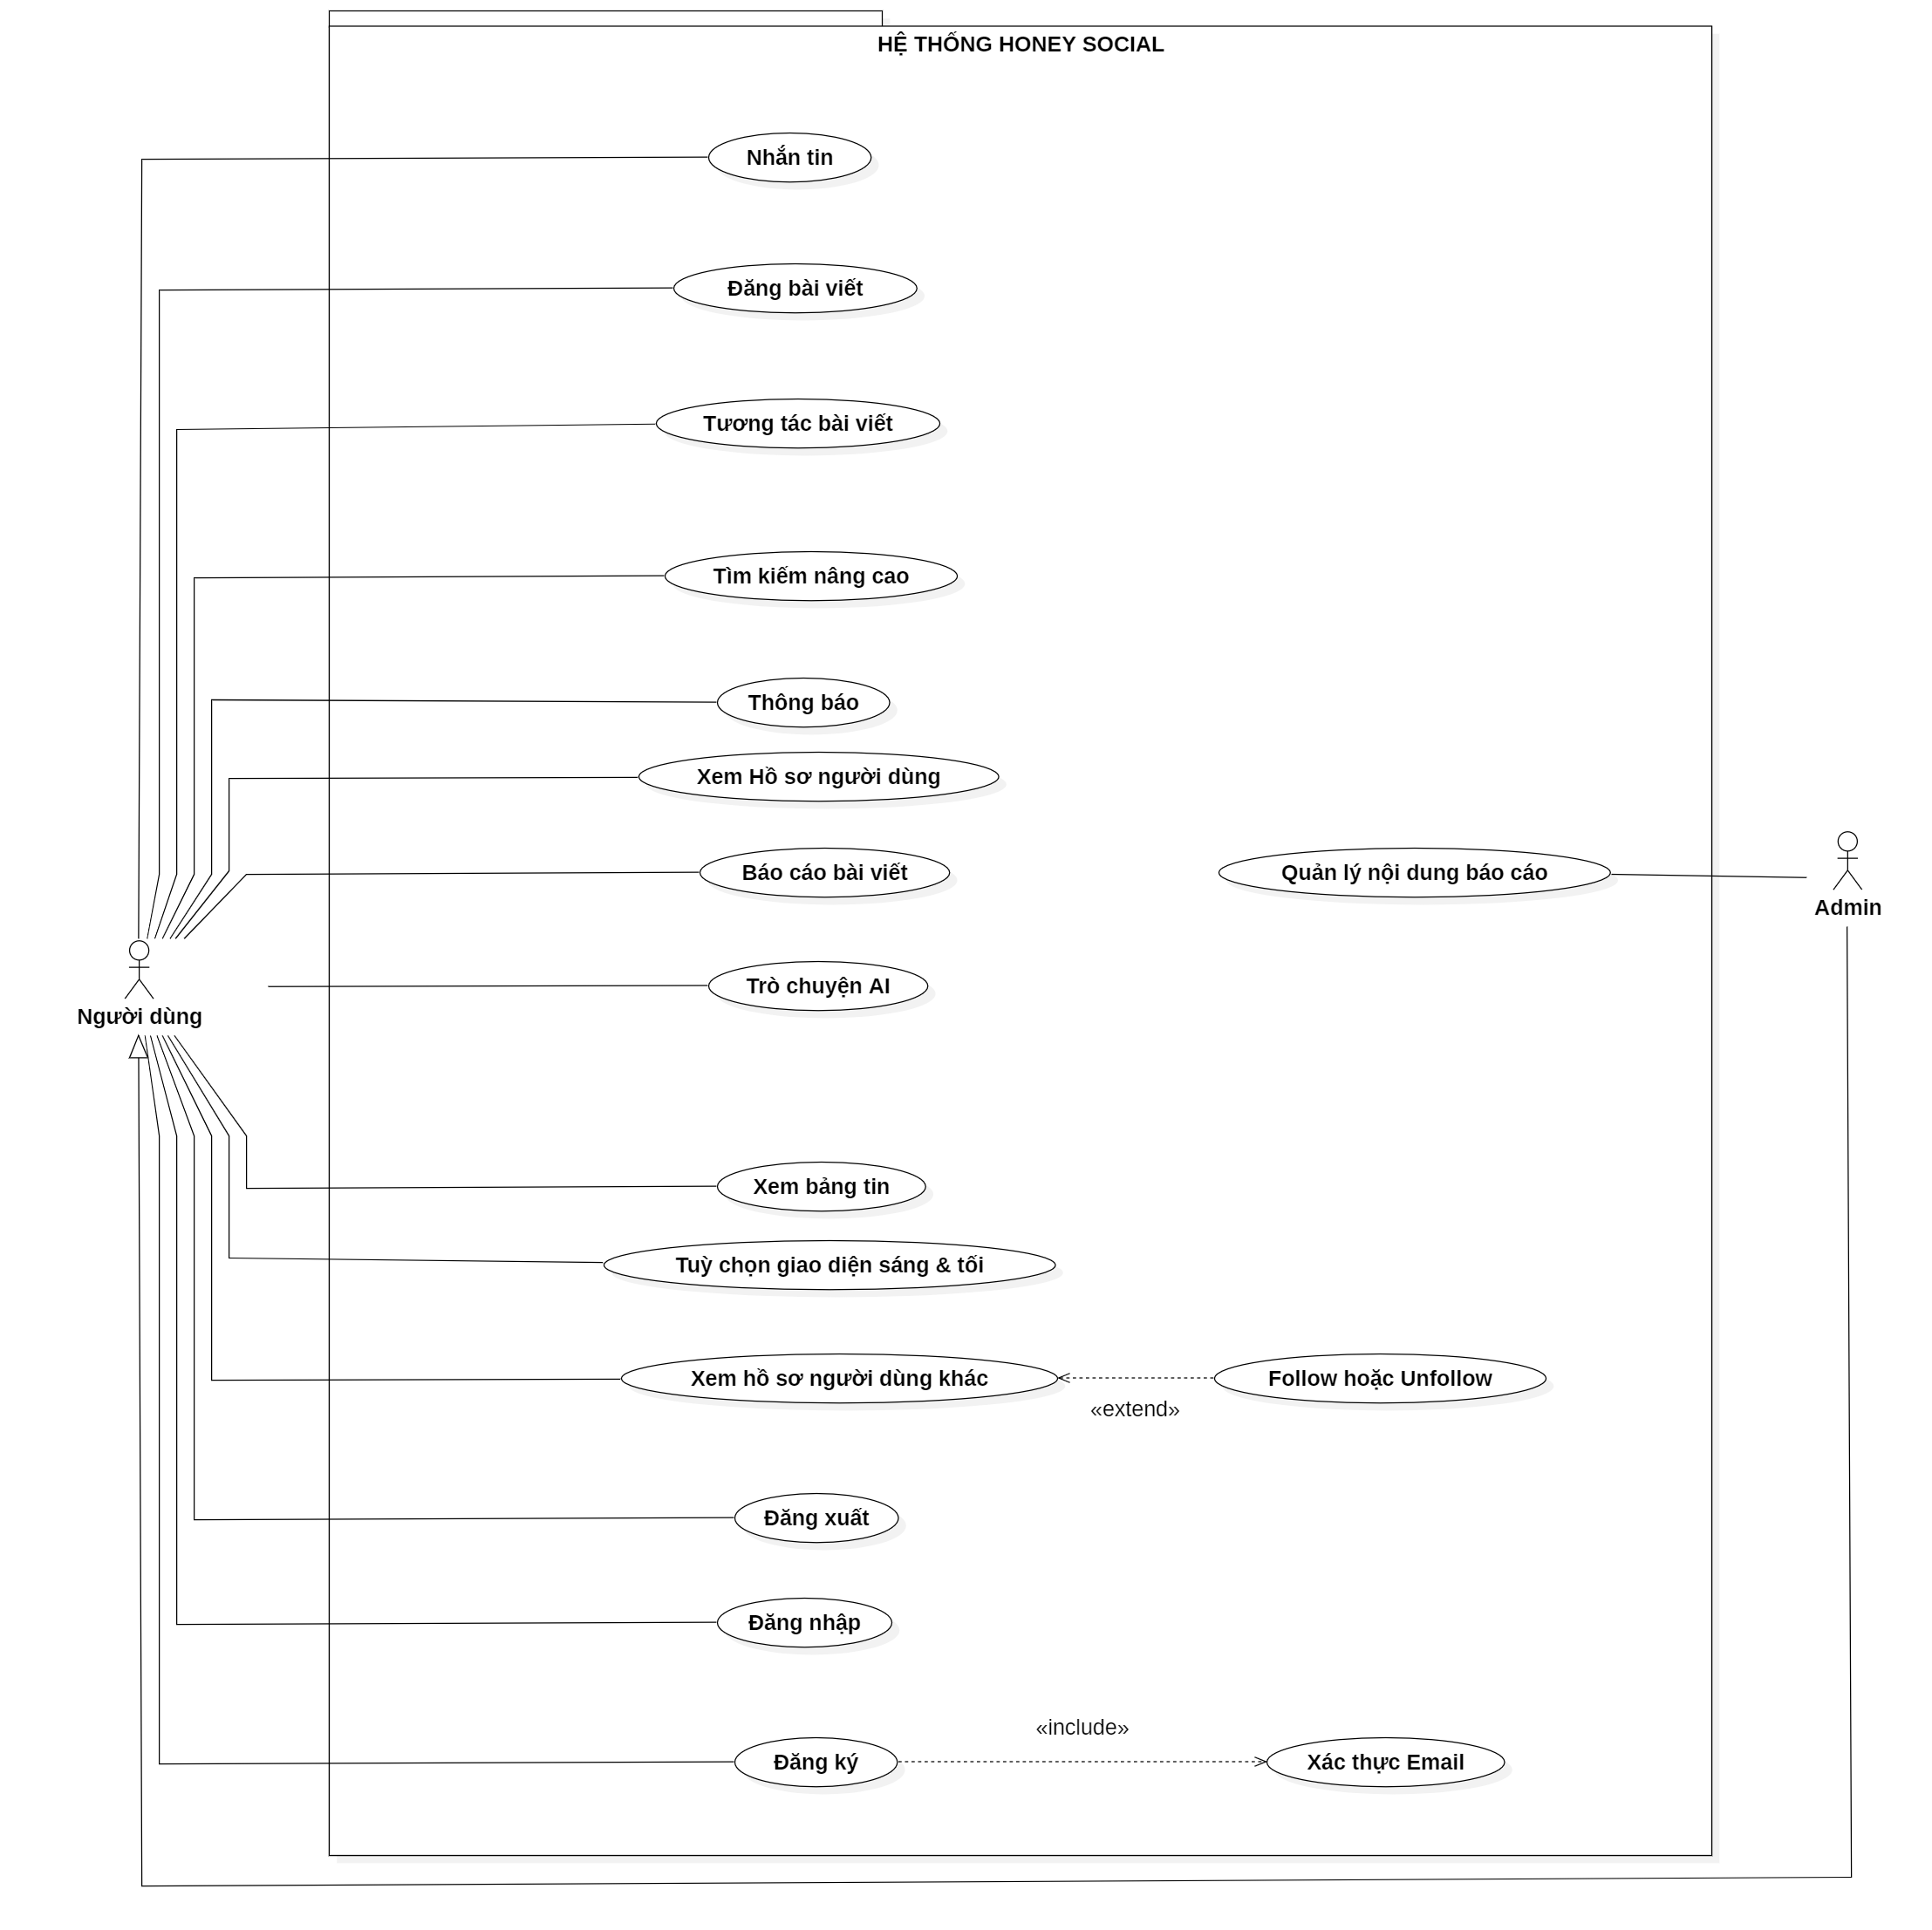
\includegraphics[width=1\textwidth]{image/MoHinh/1.png}
%     \caption{Hình ảnh Use Case Tổng quát}
%     \label{fig:use_case_tong_quat}
% \end{figure}
% Các chức năng được bao bởi hệ thống \textbf{HỆ THỐNG HONEY SOCIAL} và là những hành động mà người dùng có thể thực hiện như sau:

% \begin{itemize}
%     \item Nhắn tin
%     \item Đăng bài viết
%     \item Tương tác bài viết: Thích, bình luận, chia sẻ,...
%     \item Tìm kiếm nâng cao
%     \item Thông báo
%     \item Xem hồ sơ người dùng
%     \item Báo cáo bài viết
%     \item Trò chuyện AI
%     \item Xem bảng tin
%     \item Tùy chọn giao diện sáng \& tối
%     \item Đăng nhập
%     \item Đăng xuất
% \end{itemize}

% \textbf{Đăng bài viết} \\
% \begin{figure}[H]
%     \centering
%     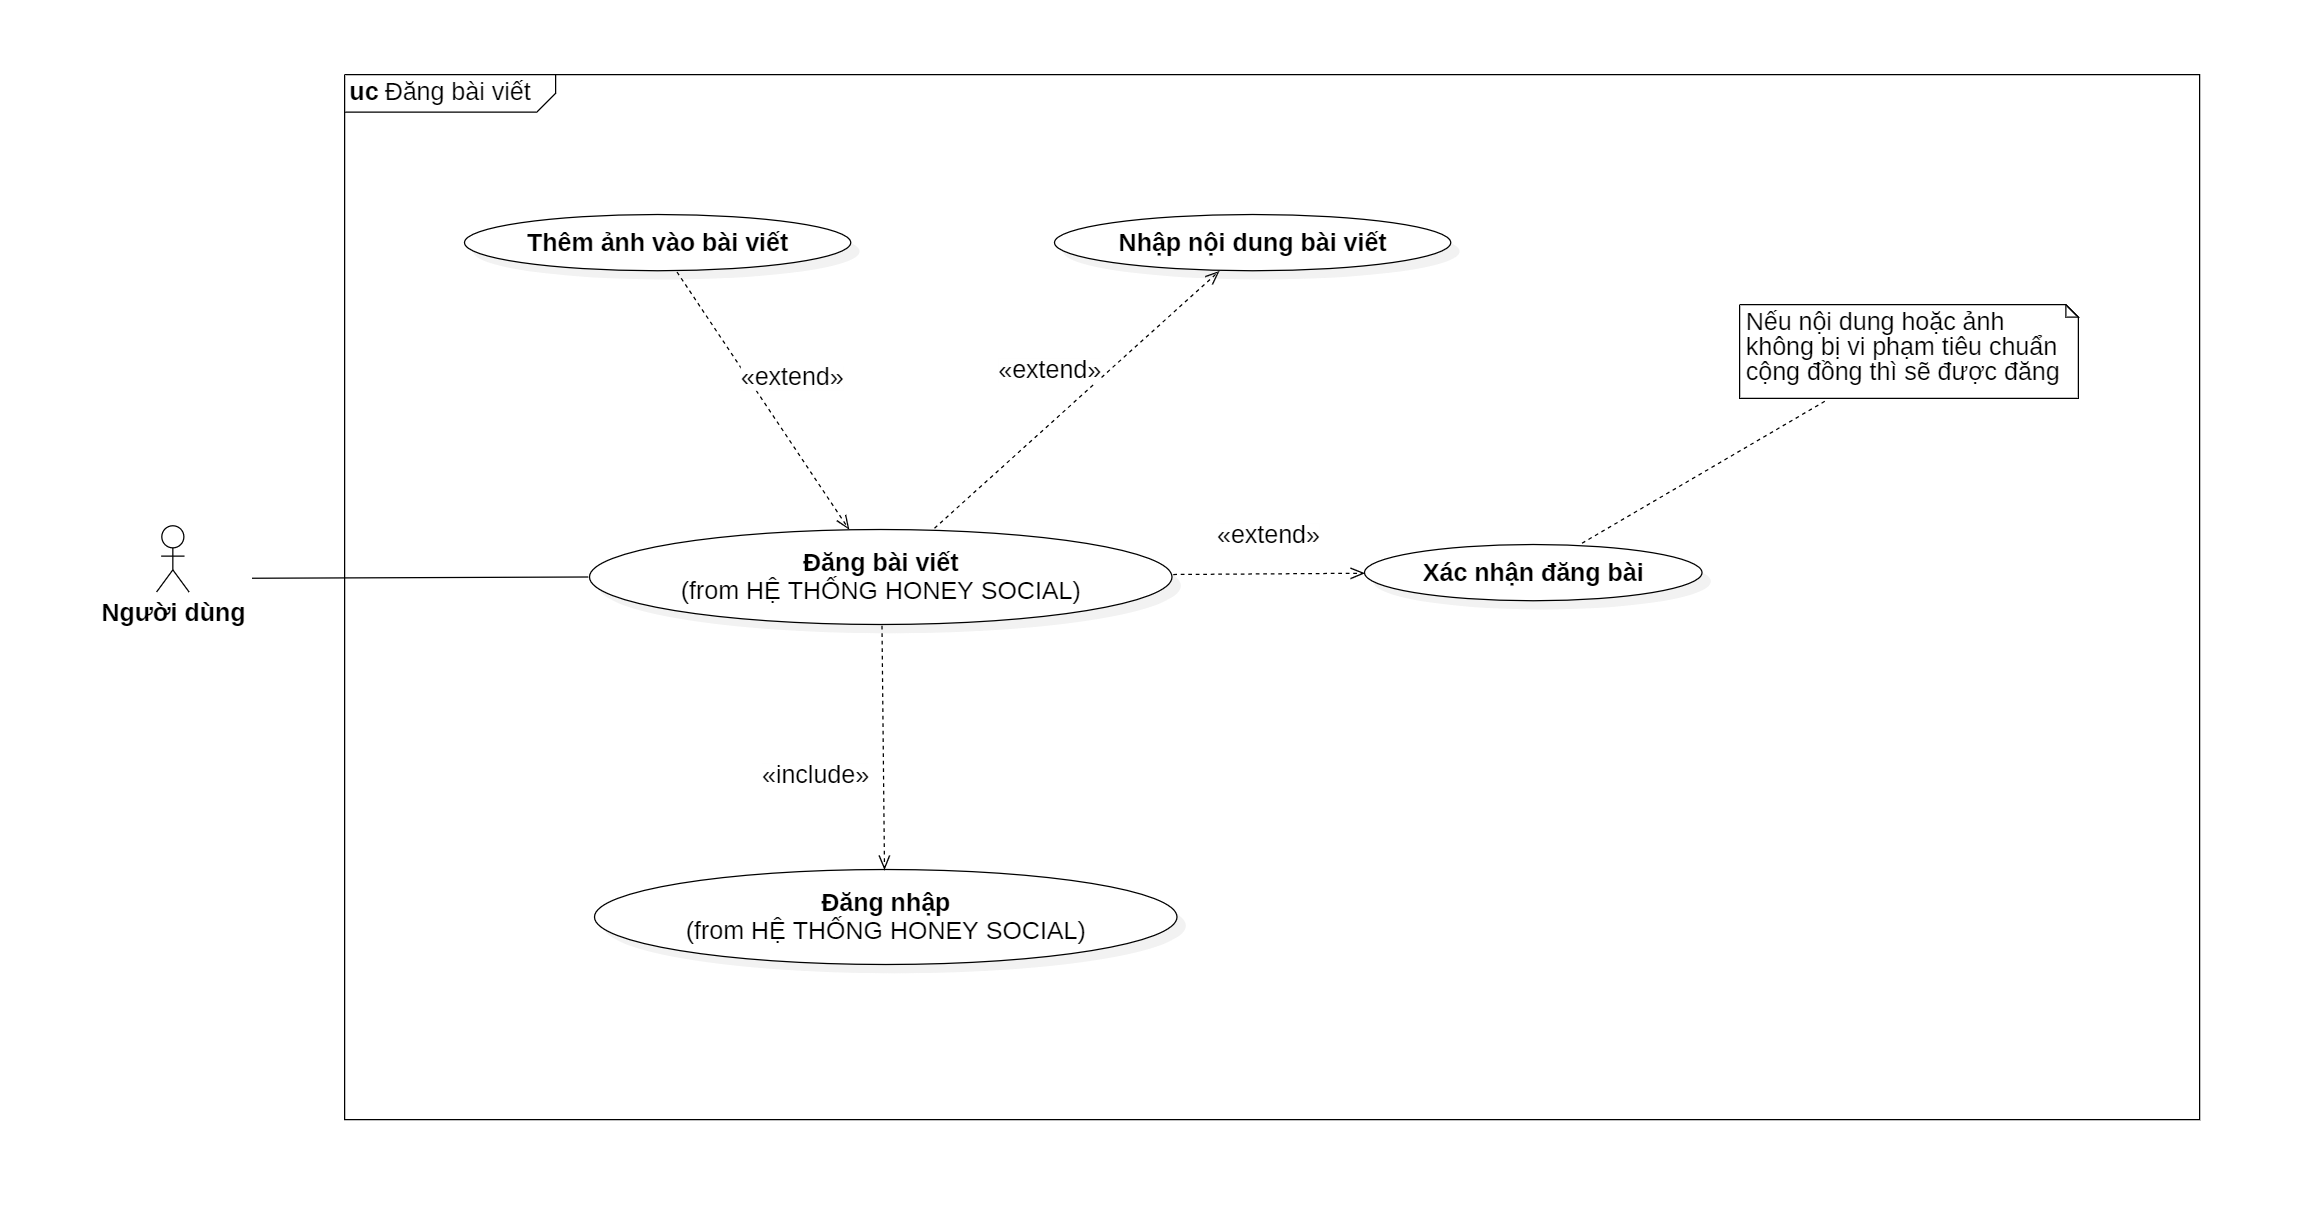
\includegraphics[width=1\textwidth]{image/MoHinh/2.png}
%     \caption{Hình ảnh Đăng bài viết}
%     \label{fig:dang_bai_viet_seq}
% \end{figure}
% Mô tả chi tiết quy trình đăng bài, bắt đầu từ việc người dùng nhập nội dung văn bản, tải lên ảnh hoặc video, chỉnh sửa trước khi đăng (bao gồm thêm hashtag hoặc thẻ người), trải qua kiểm duyệt tự động bằng AI, và cuối cùng là xác nhận để bài viết được công khai trên bảng tin.

% \textbf{Tìm kiếm nâng cao} \\
% \begin{figure}[H]
%     \centering
%     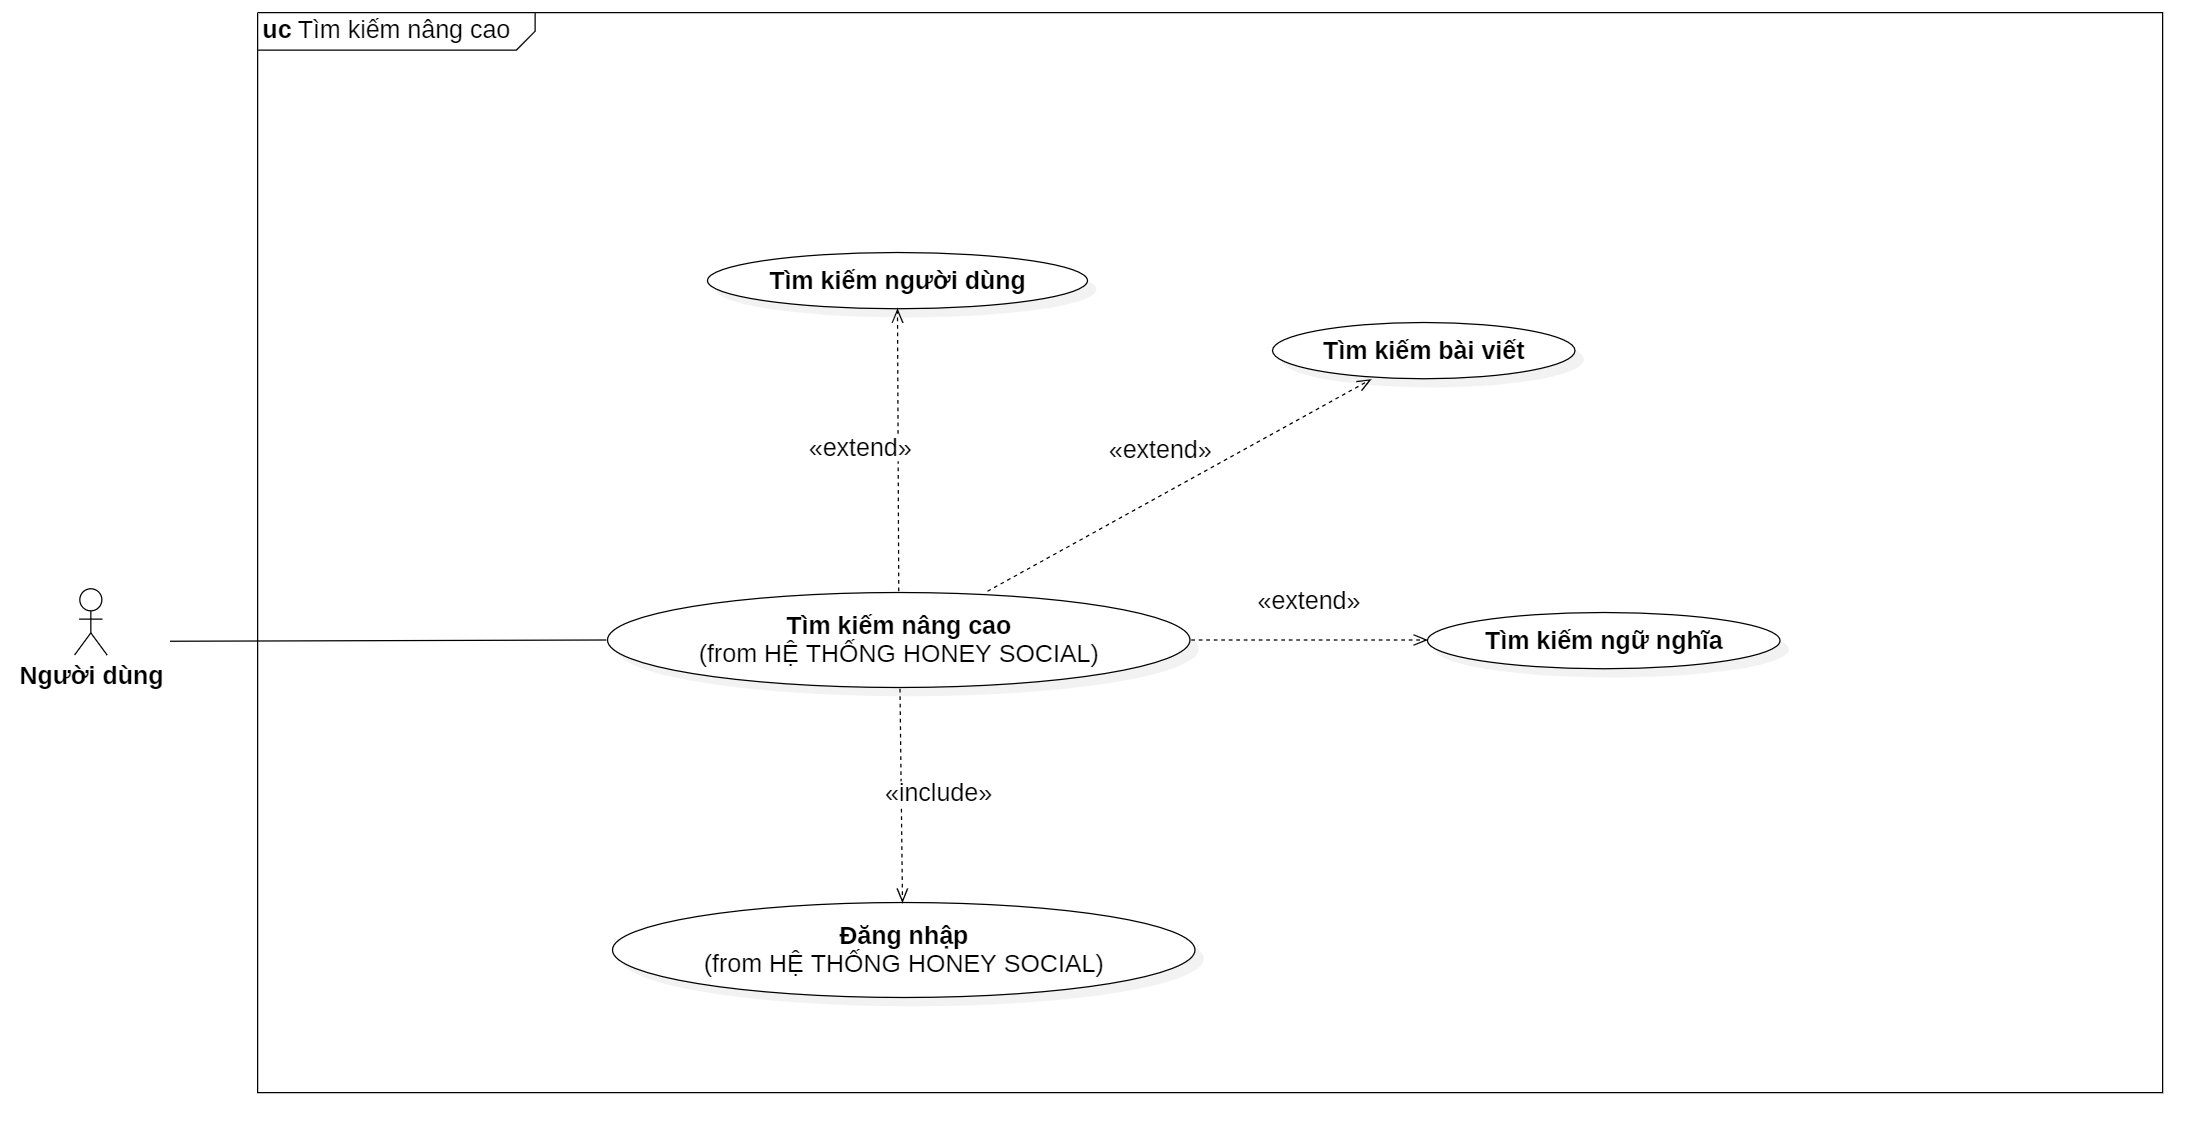
\includegraphics[width=1\textwidth]{image/MoHinh/3.png}
%     \caption{Hình ảnh Tìm kiếm nâng cao}
%     \label{fig:tim_kiem_nang_cao1}
% \end{figure}
% Hiển thị quy trình tìm kiếm thông minh, cho phép người dùng sử dụng bộ lọc theo từ khóa, thời gian, hoặc sở thích cá nhân, tích hợp gợi ý dựa trên vector similarity từ Elasticsearch, và sắp xếp kết quả theo mức độ liên quan hoặc thời gian đăng tải để tối ưu hóa trải nghiệm tìm kiếm.

% \newpage
% \textbf{Thông báo} \\
% \begin{figure}[H]
%     \centering
%     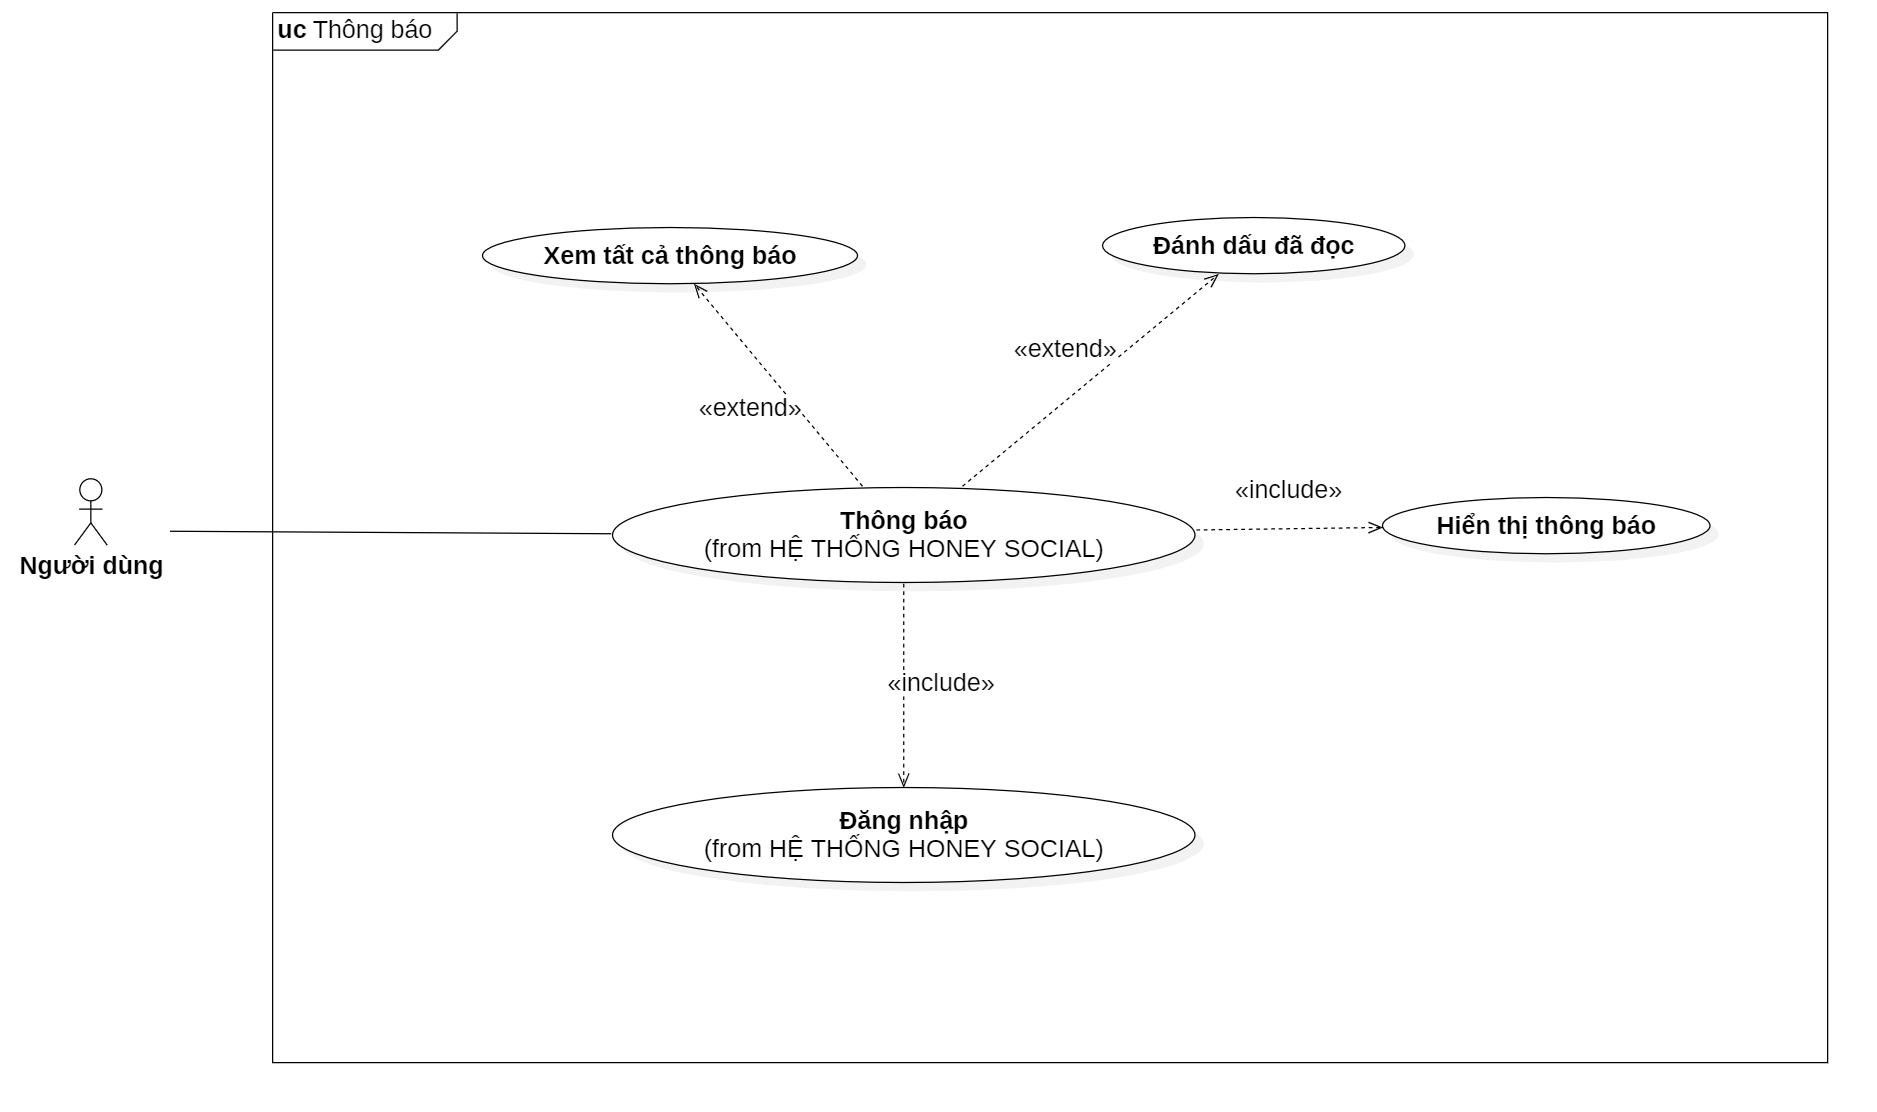
\includegraphics[width=1\textwidth]{image/MoHinh/4.png}
%     \caption{Hình ảnh Thông báo}
%     \label{fig:thong_bao}
% \end{figure}
% Chi tiết hóa cách hệ thống gửi thông báo thời gian thực, bao gồm thông báo khi có tương tác (thích, bình luận), cập nhật từ người theo dõi, hoặc thông báo hệ thống (như xác nhận email), với tùy chọn tắt/mở thông báo để cá nhân hóa trải nghiệm.

% \newpage
% \textbf{Xem hồ sơ người dùng} \\
% \begin{figure}[H]
%     \centering
%     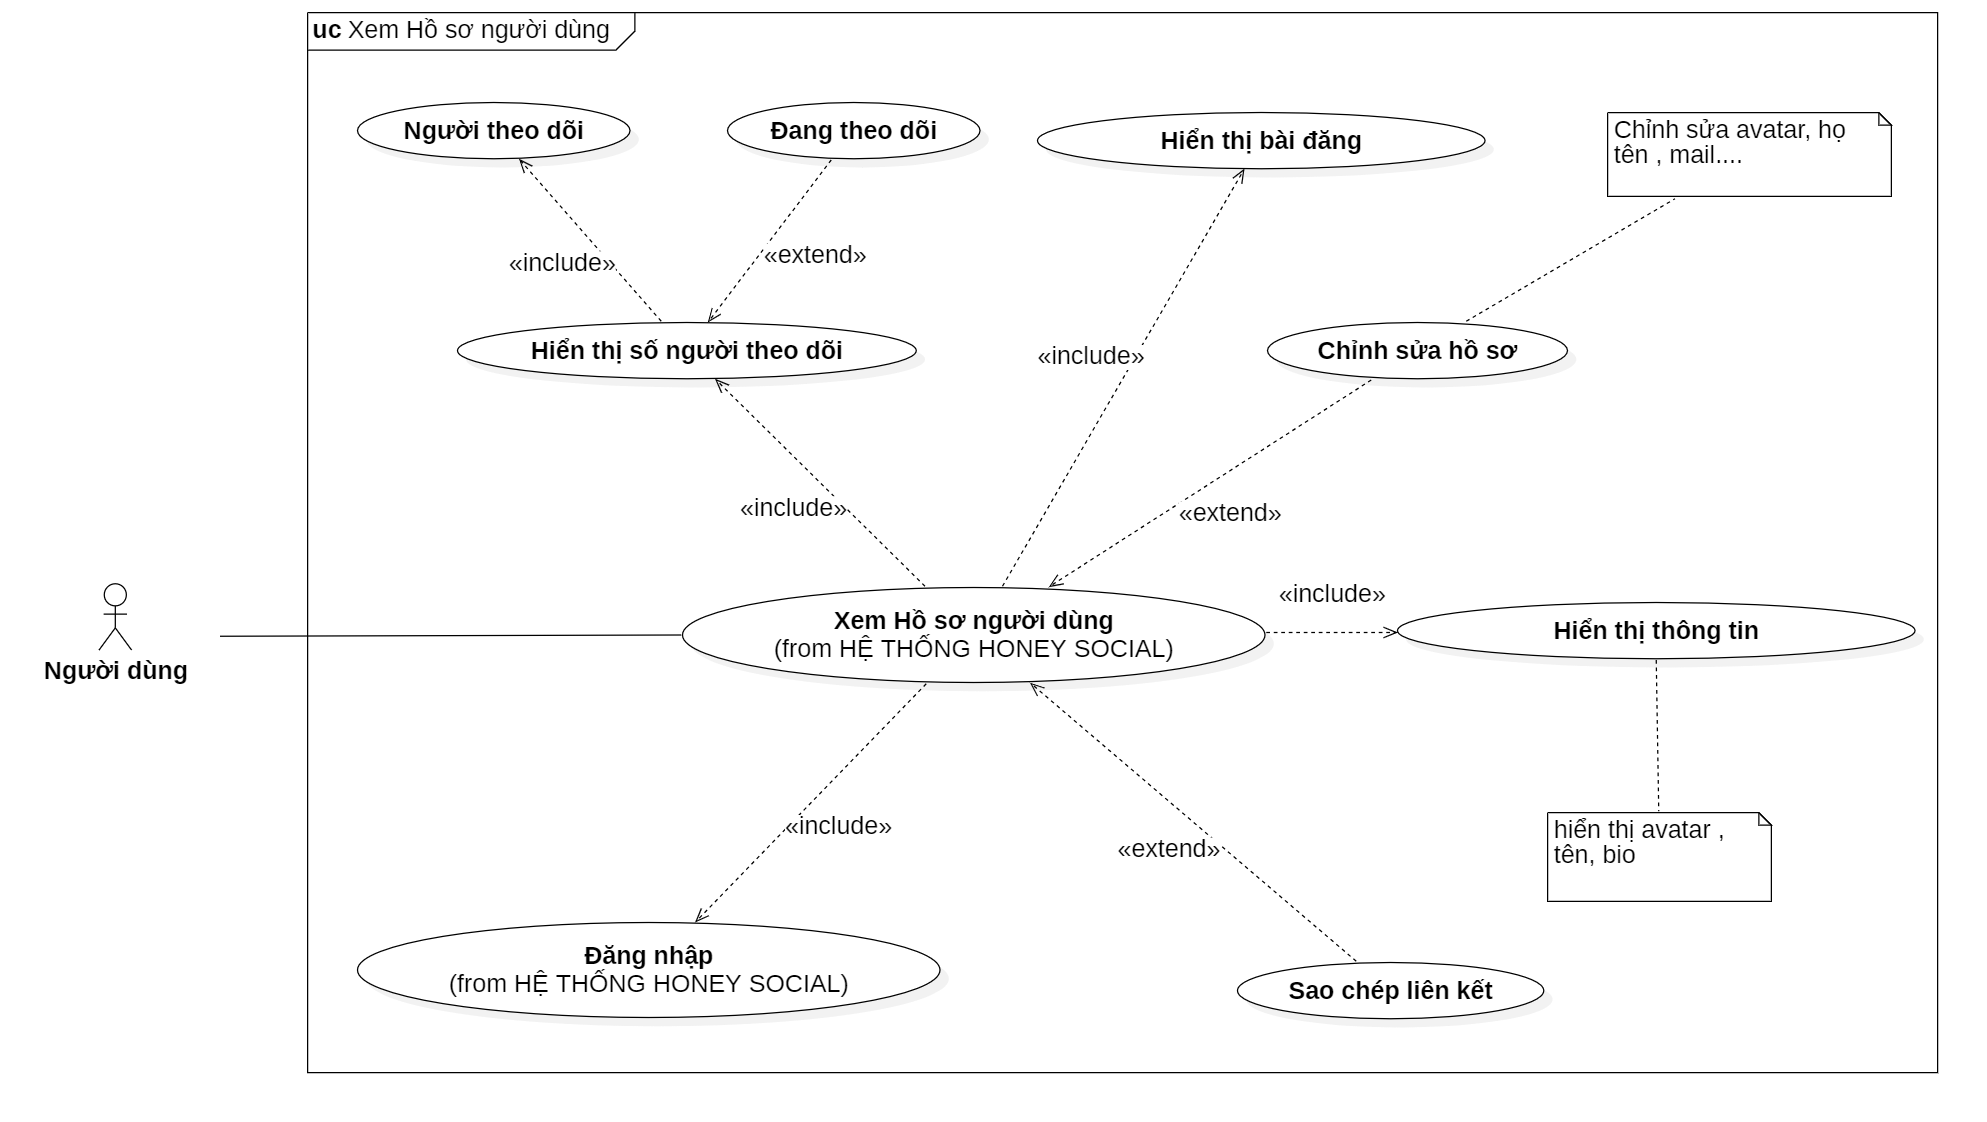
\includegraphics[width=1\textwidth]{image/MoHinh/5.png}
%     \caption{Hình ảnh Xem Hồ sơ người dùng}
%     \label{fig:xem_ho_so_nguoi_dung}
% \end{figure}
% Hướng dẫn chi tiết cách người dùng xem và chỉnh sửa hồ sơ cá nhân, bao gồm cập nhật avatar thông qua Cloudinary, chỉnh sửa thông tin như tên, bio, và danh sách theo dõi/người theo dõi, cùng với các thống kê cơ bản như số bài đăng.

% \textbf{Báo cáo bài viết} \\
% \begin{figure}[H]
%     \centering
%     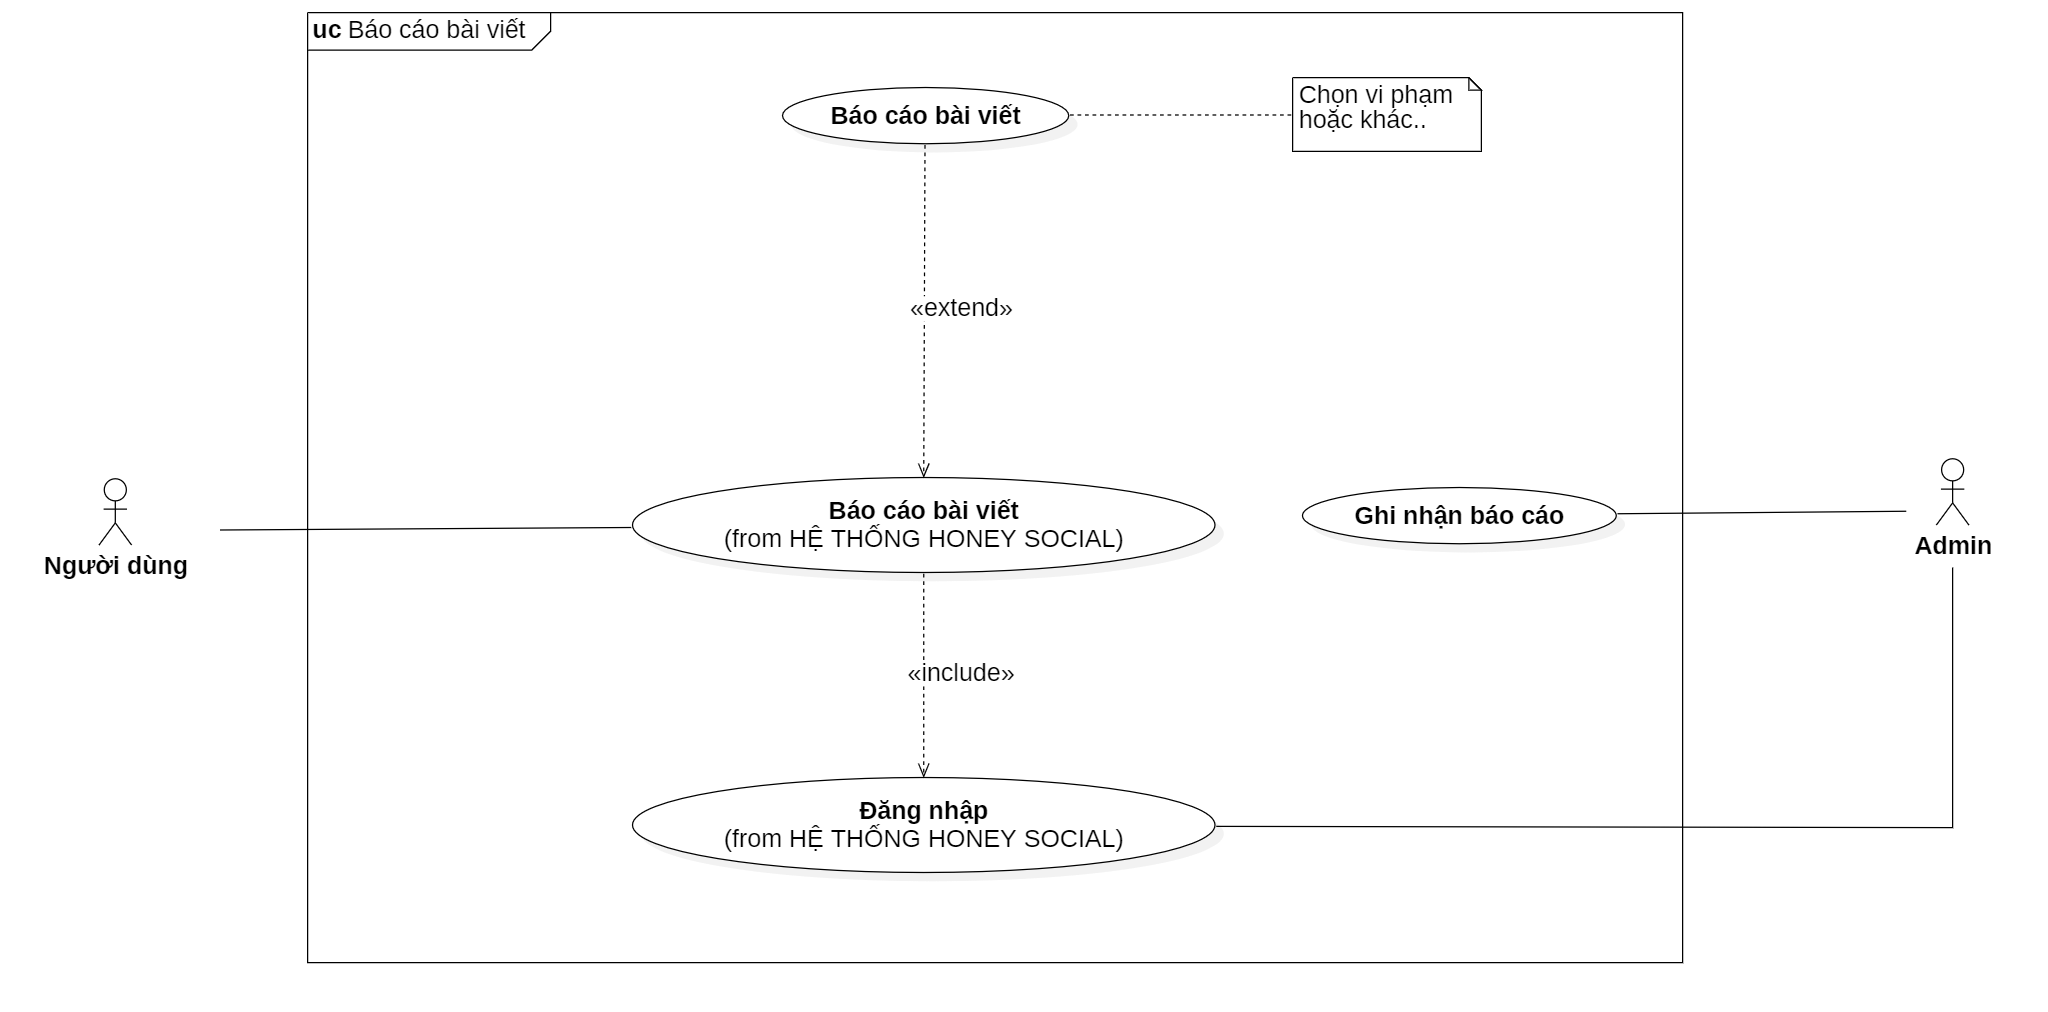
\includegraphics[width=1\textwidth]{image/MoHinh/6.png}
%     \caption{Hình ảnh Báo cáo bài viết}
%     \label{fig:bao_cao_bai_viet}
% \end{figure}
% Mô tả quy trình người dùng báo cáo vi phạm, bao gồm chọn lý do cụ thể (nội dung không phù hợp, bạo lực, spam...), gửi thông tin kèm bằng chứng qua API, và chuyển đến quản trị viên để xử lý theo các cấp độ (nhẹ, vừa, nặng).

% \textbf{Trò chuyện AI} \\
% \begin{figure}[H]
%     \centering
%     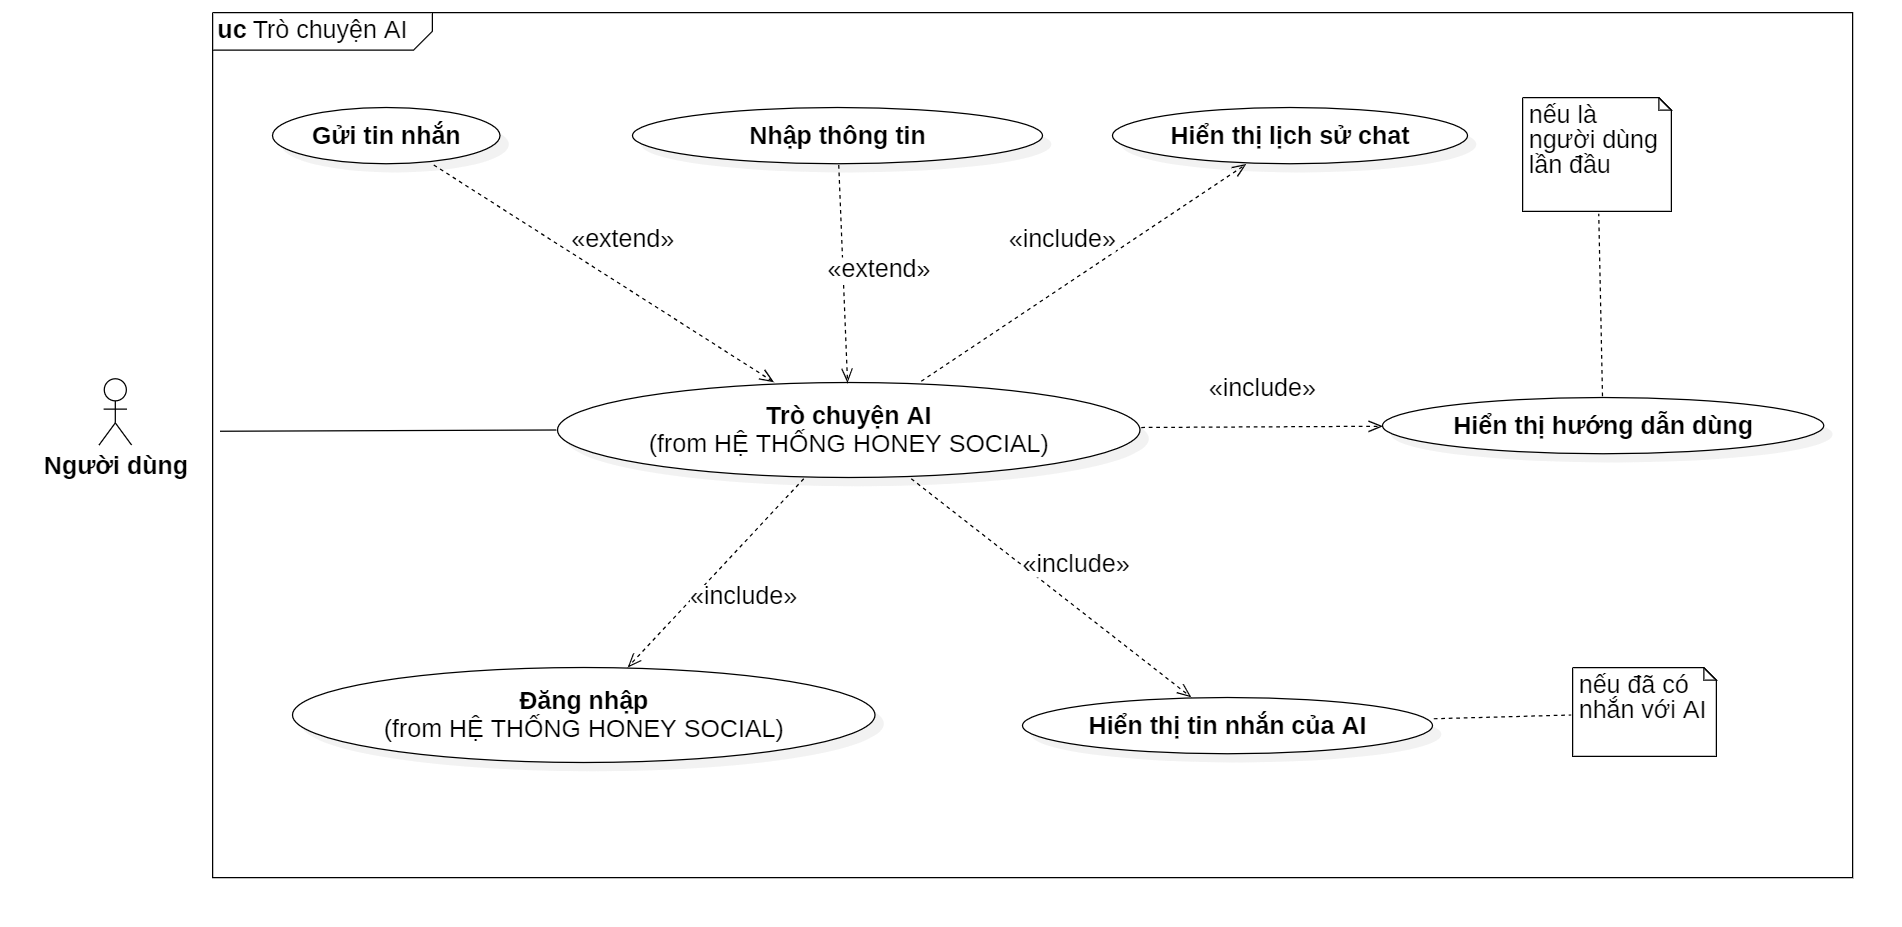
\includegraphics[width=1\textwidth]{image/MoHinh/7.png}
%     \caption{Hình ảnh Trò chuyện AI}
%     \label{fig:tro_chuyen_ai}
% \end{figure}
% Phác thảo chức năng chat AI, hỗ trợ trả lời câu hỏi liên quan đến nội dung bài viết, gợi ý bài viết dựa trên sở thích, và tự động phát hiện/phân loại báo cáo vi phạm, với giao diện thân thiện và phản hồi thời gian thực.

% \newpage
% \textbf{Xem bảng tin} \\
% \begin{figure}[H]
%     \centering
%     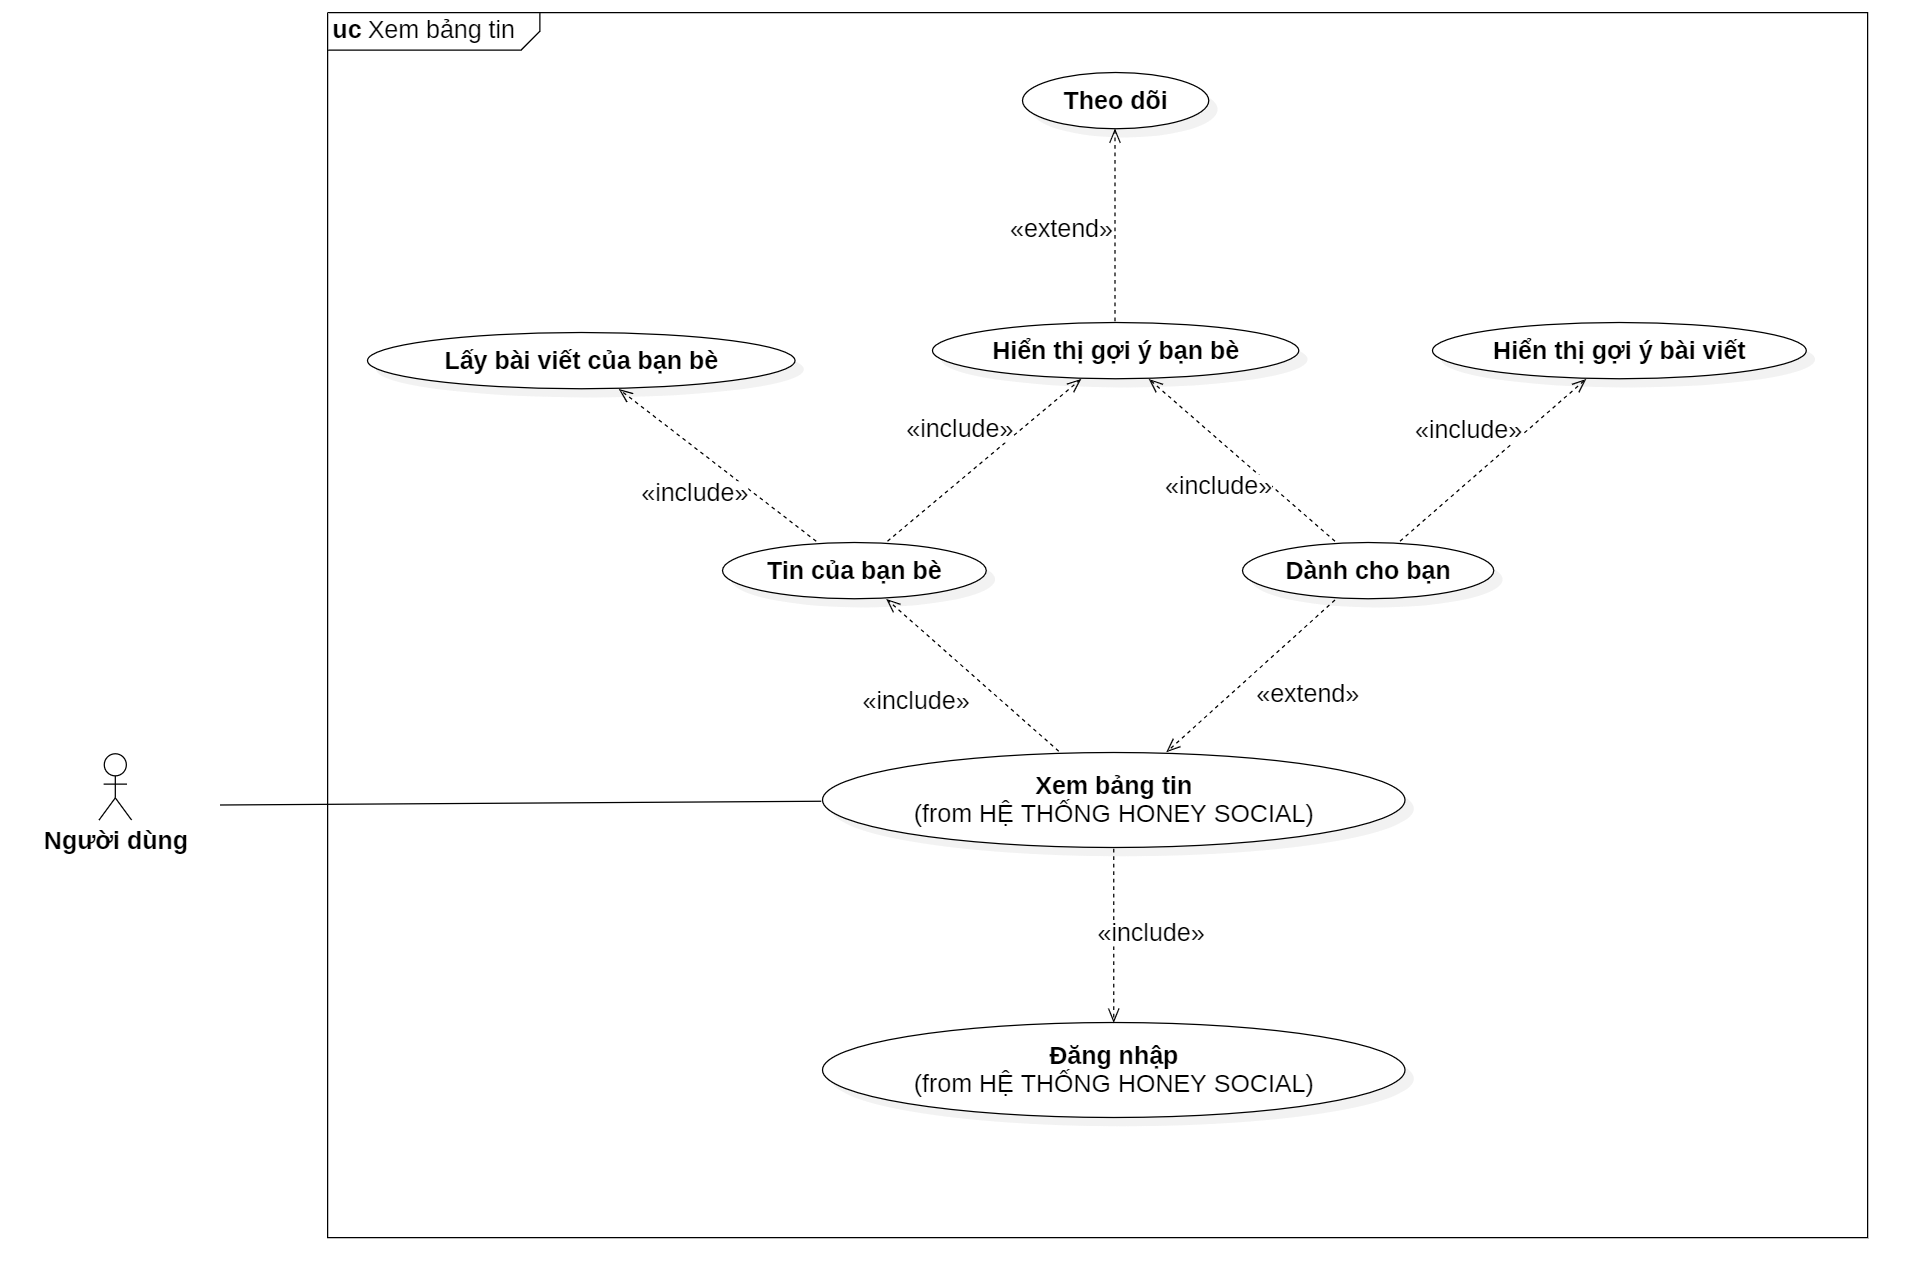
\includegraphics[width=1\textwidth]{image/MoHinh/8.png}
%     \caption{Hình ảnh Xem bảng tin}
%     \label{fig:xem_bang_tin}
% \end{figure}
% Thể hiện cách hệ thống hiển thị feed bài viết cá nhân hóa, lấy dữ liệu từ người dùng theo dõi, tích hợp gợi ý từ AI dựa trên vector nhúng, và cho phép làm mới feed hoặc lọc theo chủ đề để tăng tính tương tác.

% \textbf{Xem hồ sơ người khác} \\
% \begin{figure}[H]
%     \centering
%     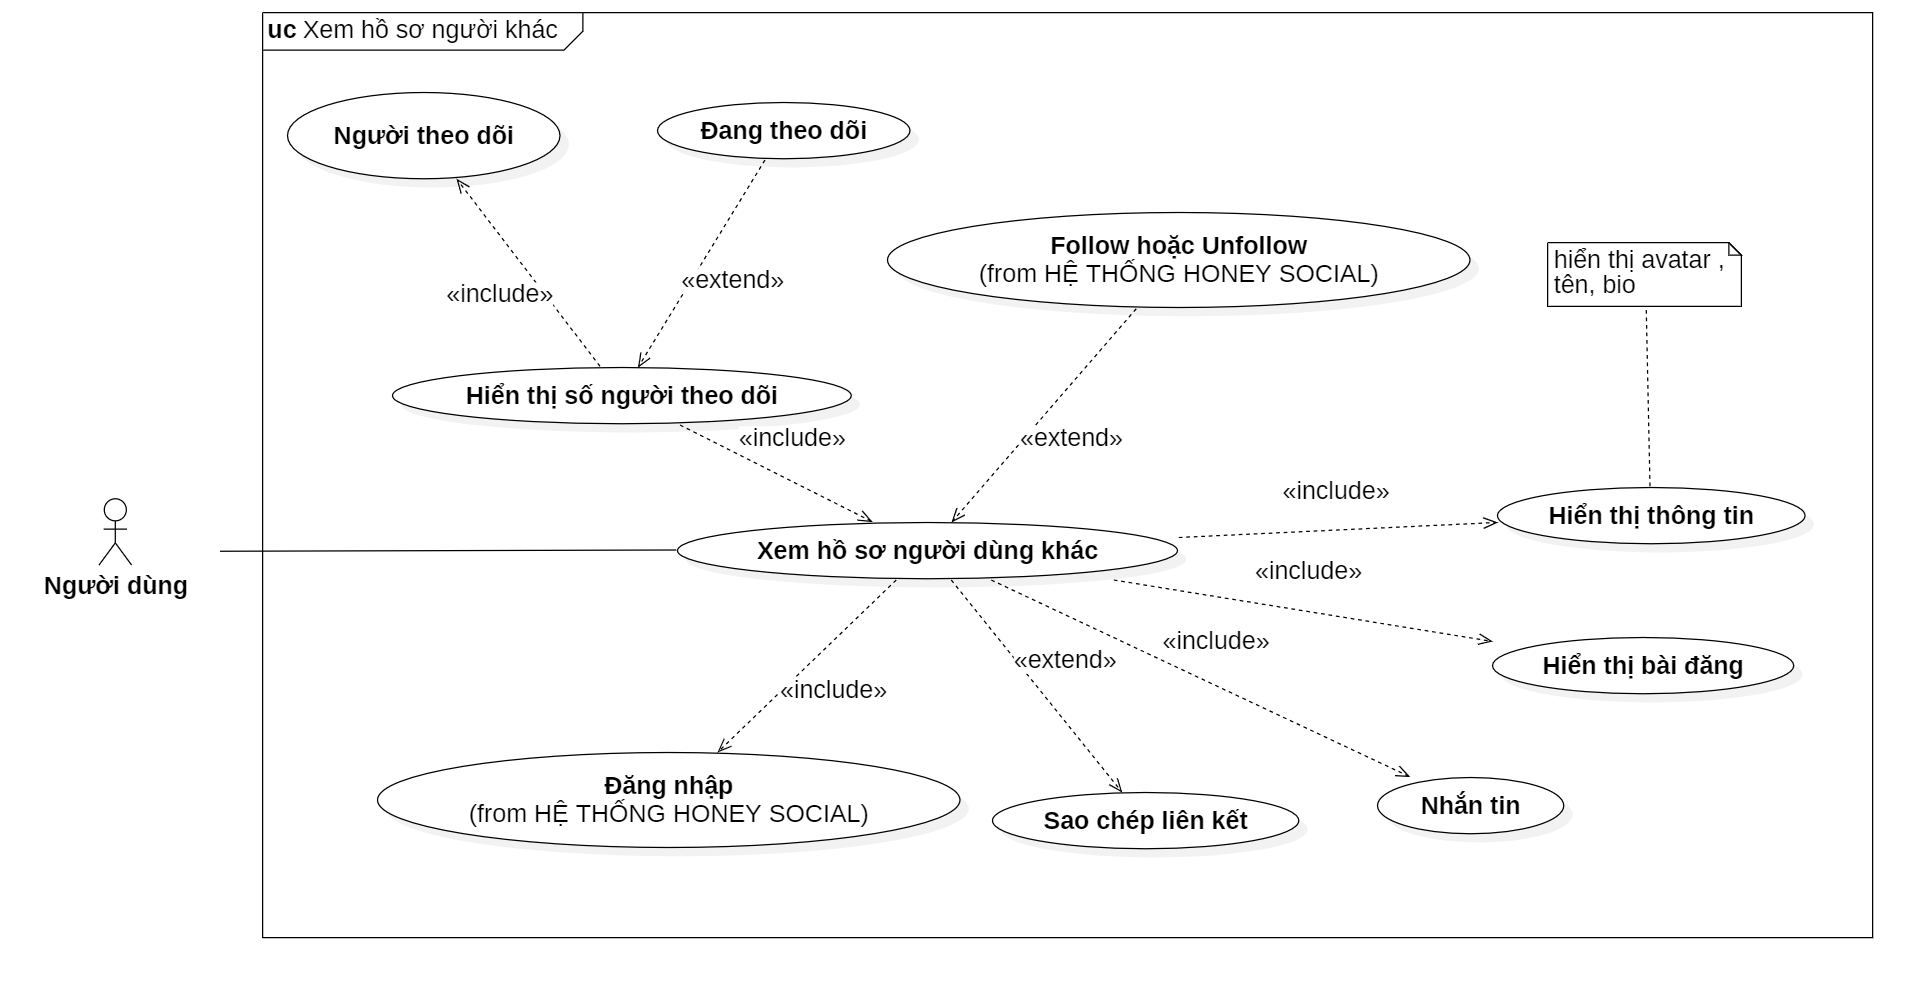
\includegraphics[width=1\textwidth]{image/MoHinh/9.png}
%     \caption{Hình ảnh Xem hồ sơ người khác}
%     \label{fig:xem_ho_so_nguoi_khac}
% \end{figure}
% Chi tiết quy trình xem hồ sơ người dùng khác, bao gồm thông tin cơ bản (tên, avatar, bio), danh sách bài đăng công khai, và các tùy chọn tương tác như theo dõi hoặc gửi tin nhắn.

% \textbf{Đăng ký} \\
% \begin{figure}[H]
%     \centering
%     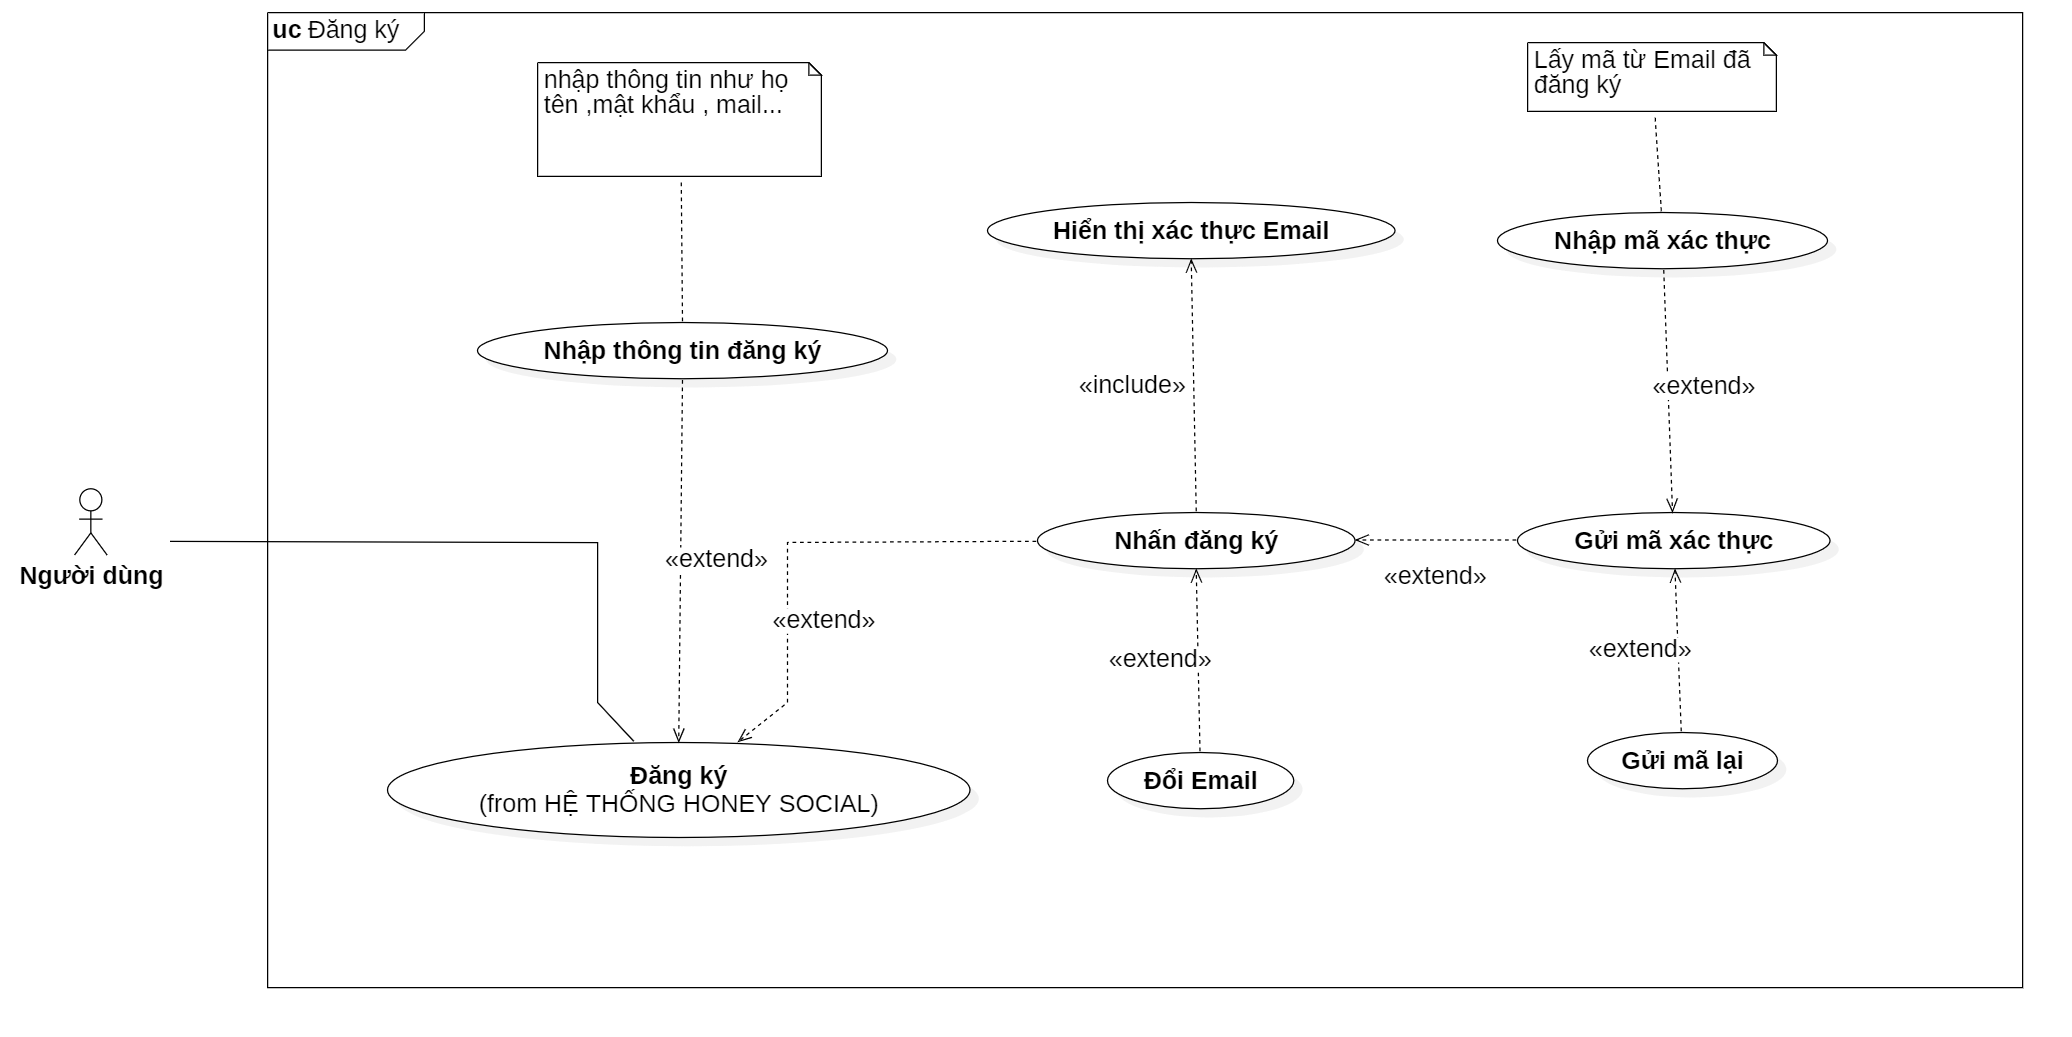
\includegraphics[width=1\textwidth]{image/MoHinh/10.png}
%     \caption{Hình ảnh Đăng ký}
%     \label{fig:dang_ky}
% \end{figure}
% Mô tả quy trình đăng ký tài khoản, yêu cầu nhập thông tin (email, mật khẩu), gửi mã OTP qua Resend API để xác thực, và hoàn tất với tùy chọn cá nhân hóa hồ sơ ngay sau đăng ký.
% \newpage
% \textbf{Quản lý nội dung báo cáo} \\
% \begin{figure}[H]
%     \centering
%     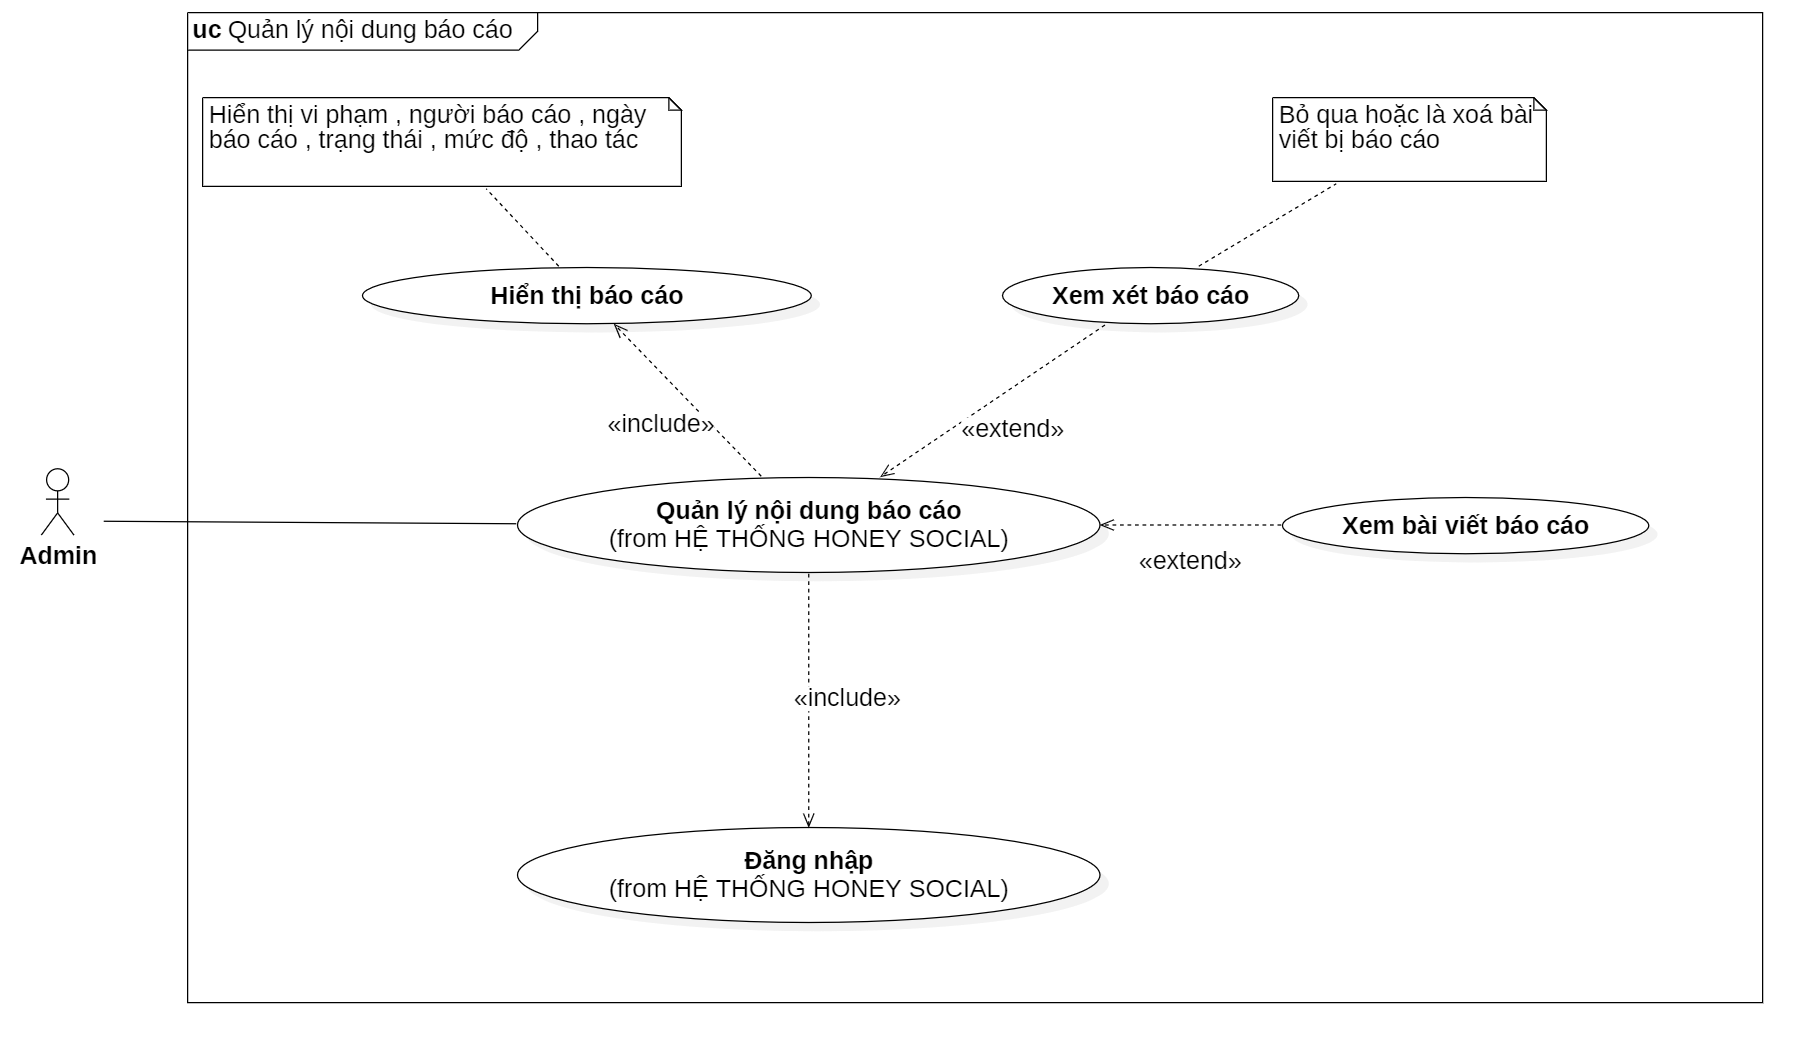
\includegraphics[width=1\textwidth]{image/MoHinh/11.png}
%     \caption{Hình ảnh Quản lý nội dung báo cáo}
%     \label{fig:quan_ly_noi_dung_bao_cao}
% \end{figure}
% Hiển thị cách quản trị viên tiếp nhận báo cáo từ người dùng, phân loại theo mức độ vi phạm (nhẹ: cảnh báo; vừa: ẩn bài; nặng: xóa và khóa tài khoản), và xử lý qua dashboard admin với các công cụ lọc theo thời gian hoặc lý do.
% \newpage
% \textbf{Tương tác bài viết} \\
% \begin{figure}[H]
%     \centering
%     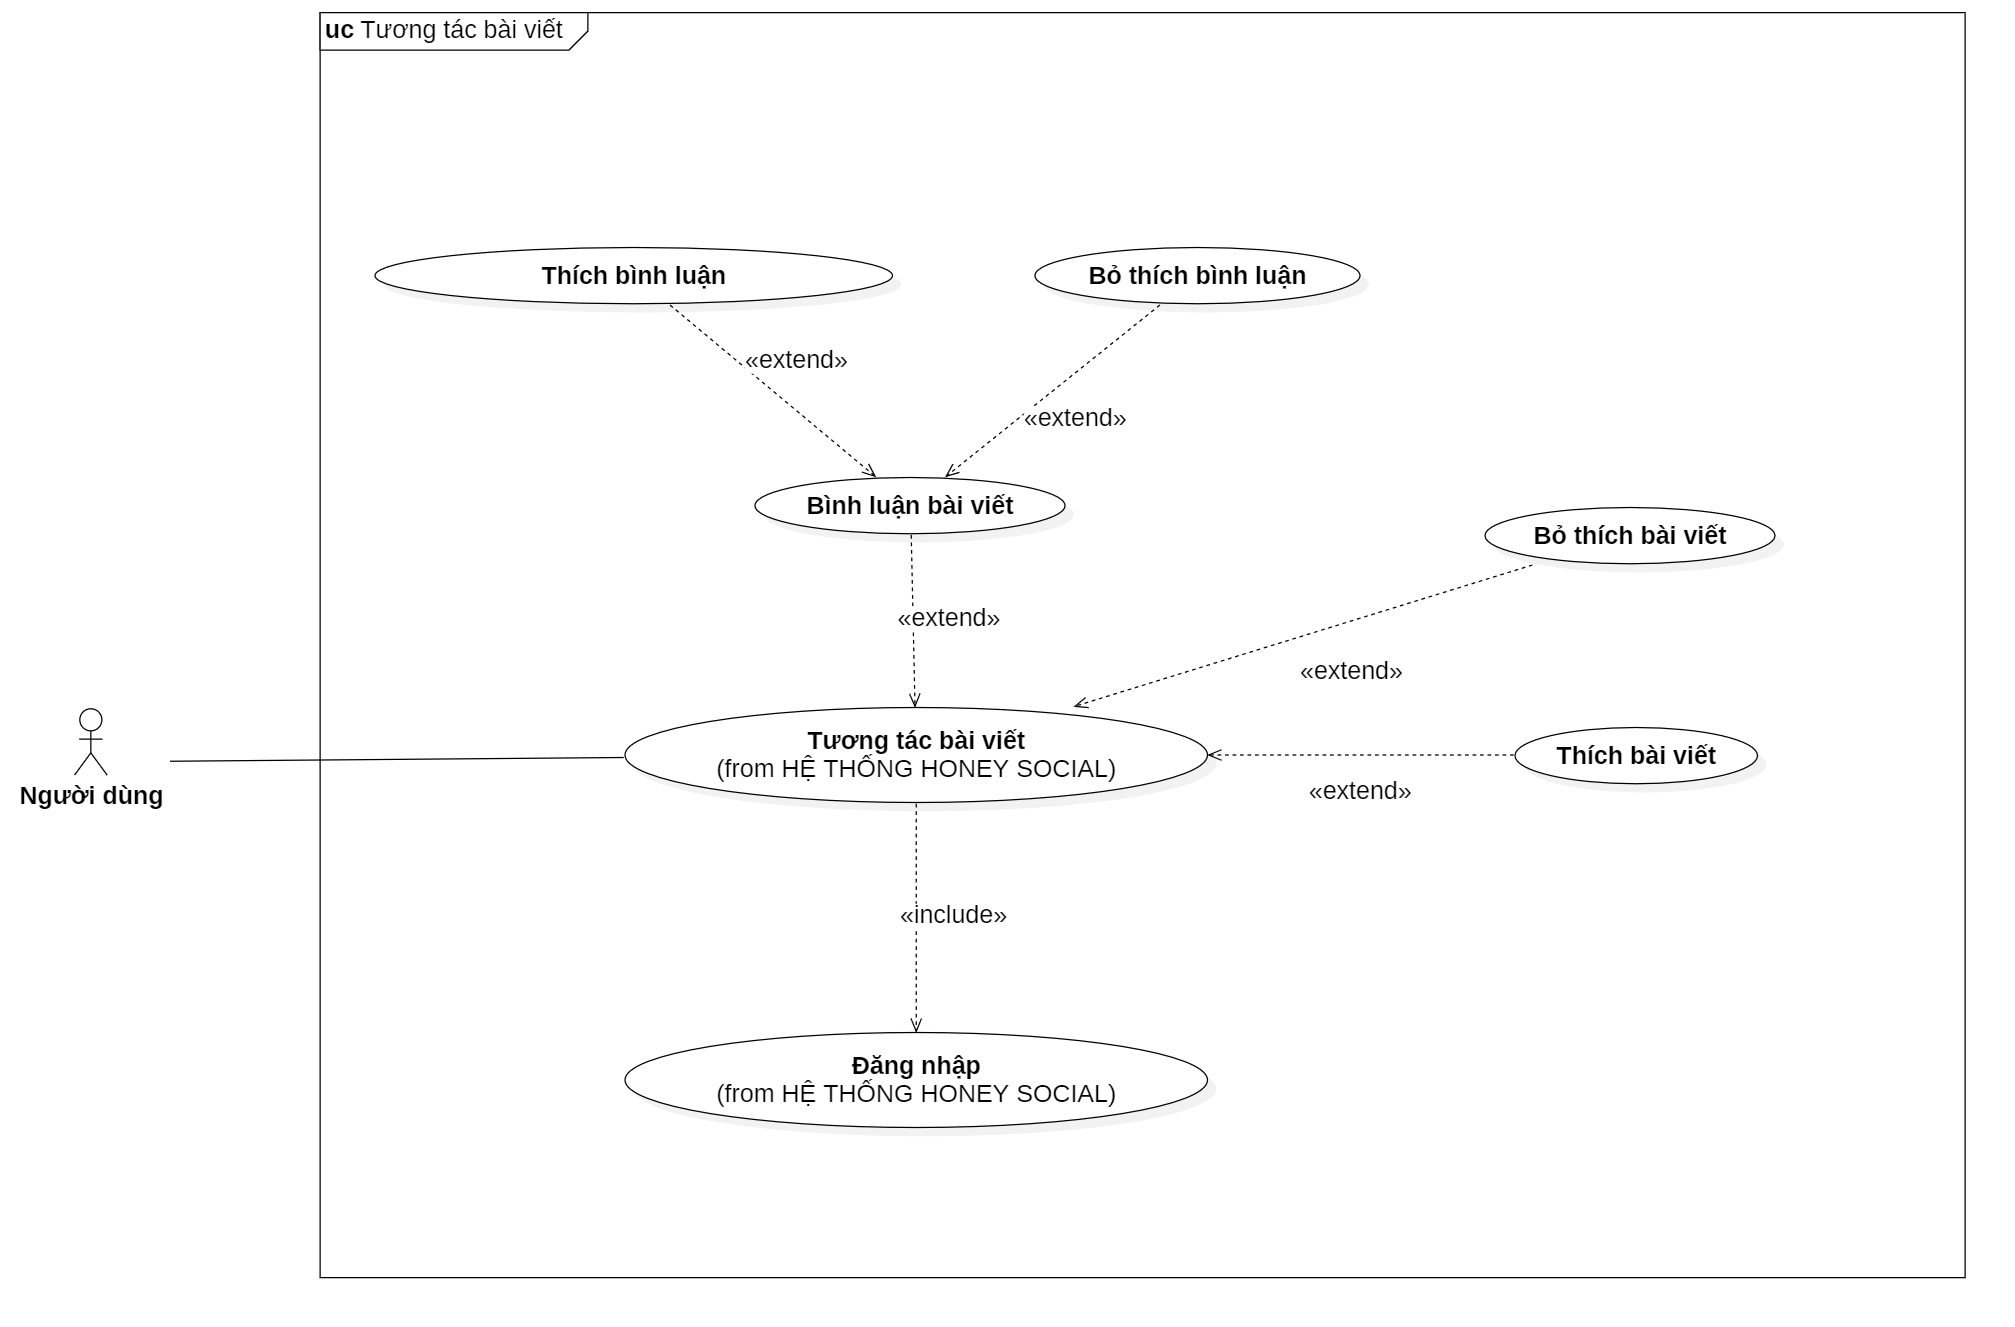
\includegraphics[width=1\textwidth]{image/MoHinh/12.png}
%     \caption{Hình ảnh Tương tác bài viết}
%     \label{fig:tuong_tac_bai_viet}
% \end{figure}
% Phác thảo các hành động tương tác như thích (like), bình luận (với khả năng phản hồi), và chia sẻ liên kết bài viết ra ngoài, tất cả đều được xử lý qua Socket.IO để đảm bảo cập nhật thời gian thực.

% \newpage

% \subsubsection{Kịch bản của các UseCase}


% \begin{longtable}{|>{\bfseries}m{4cm}|m{10cm}|}
% \caption{Bảng thông tin hoạt động của chức năng đăng bài viết}
% \label{table:usecase-postsa}\\
% \hline
% Use-case name & Đăng bài viết \\ 
% \hline 
% Description & Người dùng đăng một bài viết mới lên hệ thống, có thể kèm hình ảnh.\\
% \hline
% Actor & Người dùng đã đăng nhập\\
% \hline
% Pre-Conditions & -Người dùng đã đăng nhập vào hệ thống.

% -Email của người dùng đã được xác thực (nếu hệ thống yêu cầu).\\
% \hline
% Post-Condition & -Bài viết mới được lưu vào hệ thống và hiển thị trên bảng tin.

% -Nếu có lỗi, thông báo lỗi được hiển thị cho người dùng.\\
% \hline
% Trigger & Người dùng nhấn nút "Tạo bài viết mới" hoặc biểu tượng "+".\\
% \hline
% Normal Flow &
% \begin{enumerate}
%     \item Người dùng nhấn nút "Tạo bài viết mới".
%     \item Hệ thống hiển thị modal nhập nội dung bài viết.
%     \item Người dùng nhập nội dung, chọn hình ảnh (nếu muốn).
%     \item Người dùng nhấn nút "Đăng".
%     \item Hệ thống kiểm tra điều kiện (đăng nhập, xác thực email, nội dung hợp lệ).
%     \item Nếu hợp lệ, bài viết được lưu và hiển thị; thông báo thành công cho người dùng.
% \end{enumerate} \\
% \hline
% Alternative Flow & Nếu người dùng chưa đăng nhập: Hệ thống thông báo và chuyển hướng đến trang đăng nhập.

% Nếu email chưa xác thực: Hệ thống thông báo yêu cầu xác thực email.

% Nếu nội dung vi phạm hoặc lỗi khác: Hệ thống hiển thị thông báo lỗi chi tiết.

% Nếu người dùng nhấn "Hủy": Modal đóng, không lưu bài viết.\\
% \hline
% \end{longtable}


% % \subsubsubsection{Chức năng tìm kiếm nâng cao}
% \begin{longtable}{|>{\bfseries}m{4cm}|m{10cm}|}
% \caption{Bảng thông tin hoạt động của chức năng tìm kiếm nâng cao}
% \label{table:usecase-search}\\
% \hline
% Use-case name & Tìm kiếm nâng cao
% \\
% \hline
% Description & Người dùng thực hiện tìm kiếm nâng cao để tìm kiếm người dùng, bài viết hoặc theo ngữ nghĩa trên hệ thống.\\
% \hline
% Actor & Người dùng đã đăng nhập
% \\
% \hline
% Pre-Conditions & Người dùng đã đăng nhập vào hệ thống.

% Hệ thống có dữ liệu người dùng/bài viết.\\
% \hline
% Post-Condition & Kết quả tìm kiếm được hiển thị cho người dùng theo tiêu chí đã chọn.

% Người dùng có thể chuyển trang, sắp xếp hoặc chọn kết quả để xem chi tiết.\\
% \hline
% Trigger & Người dùng truy cập trang tìm kiếm nâng cao hoặc nhập từ khóa vào ô tìm kiếm.
% \\
% \hline
% Normal Flow &
% \begin{enumerate}
%     \item Người dùng truy cập chức năng tìm kiếm nâng cao.
%     \item Người dùng nhập từ khóa tìm kiếm.
%     \item Hệ thống gửi yêu cầu tìm kiếm đến server với từ khóa và các tham số (phân trang, sắp xếp).
%     \item Server xử lý và trả về danh sách kết quả phù hợp.
%     \item Hệ thống hiển thị kết quả tìm kiếm cho người dùng, kèm số lượng và các tuỳ chọn sắp xếp.
%     \item Người dùng có thể chuyển trang, thay đổi tiêu chí sắp xếp hoặc nhấn vào kết quả để xem chi tiết.
% \end{enumerate} \\
% \hline
% Alternative Flow & Nếu người dùng chưa đăng nhập: Hệ thống yêu cầu đăng nhập trước khi sử dụng tìm kiếm nâng cao.


% Nếu không có kết quả phù hợp: Hệ thống hiển thị thông báo "Không tìm thấy người dùng phù hợp".


% Nếu xảy ra lỗi server hoặc kết nối: Hệ thống hiển thị thông báo lỗi cho người dùng.\\
% \hline
% \end{longtable}

% % \subsubsubsection{Chức năng thông báo}
% \begin{longtable}{|>{\bfseries}m{4cm}|m{10cm}|}
% \caption{Bảng thông tin hoạt động của chức năng thông báo}
% \label{table:usecase-noti}\\
% \hline

% Use-case name & Thông báo
% \\
% \hline
% Description & Người dùng xem danh sách thông báo, đánh dấu thông báo đã đọc hoặc xem chi tiết thông báo.\\
% \hline
% Actor & Người dùng đã đăng nhập\\
% \hline
% Pre-Conditions & Người dùng đã đăng nhập vào hệ thống.

% Hệ thống có thông báo liên quan đến người dùng.\\
% \hline
% Post-Condition & Thông báo được hiển thị cho người dùng.

% Thông báo được đánh dấu là đã đọc (nếu người dùng thực hiện hành động này).\\
% \hline
% Trigger & Người dùng nhấn vào biểu tượng thông báo trên giao diện.\\
% \hline
% Normal Flow &
% \begin{enumerate}
%     \item Người dùng nhấn vào biểu tượng thông báo.
%     \item Hệ thống hiển thị danh sách thông báo.
%     \item Người dùng chọn một thông báo để xem chi tiết.
%     \item Hệ thống đánh dấu thông báo đã đọc và hiển thị nội dung chi tiết.
%     \item Người dùng quay lại danh sách thông báo hoặc tiếp tục sử dụng hệ thống.
% \end{enumerate} \\
% \hline
% Alternative Flow & Nếu không có thông báo: Hệ thống hiển thị thông báo "Không có thông báo mới".

% Nếu người dùng chưa đăng nhập: Hệ thống yêu cầu người dùng đăng nhập để xem thông báo.\\
% \hline
% \end{longtable}

% % \subsubsubsection{Chức năng xem hồ sơ người dùng}

% \begin{longtable}{|>{\bfseries}m{4cm}|m{10cm}|}
%     \caption{Bảng thông tin hoạt động của chức năng xem hồ sơ người dùng}
%     \label{table:usecase-profile}\\

% \hline
% Use-case name & Xem hồ sơ người dùng \\
% \hline
% Description & Người dùng có thể xem hồ sơ của bản thân hoặc người dùng khác, bao gồm thông tin cá nhân, danh sách bài đăng, số lượng người theo dõi và đang theo dõi. \\
% \hline
% Actor & Người dùng đã đăng nhập \\
% \hline
% Pre-Conditions & 
% \begin{itemize}
%     \item Người dùng đã đăng nhập vào hệ thống.
%     \item Hồ sơ của người dùng hoặc người khác tồn tại trong hệ thống.
% \end{itemize} \\
% \hline
% Post-Condition & 
% \begin{itemize}
%     \item Hồ sơ người dùng được hiển thị đầy đủ thông tin.
%     \item Người dùng có thể thực hiện các hành động như theo dõi, nhắn tin, hoặc chỉnh sửa hồ sơ (nếu là hồ sơ của chính họ).
% \end{itemize} \\
% \hline
% Trigger & Người dùng nhấn vào tên hoặc ảnh đại diện của một người dùng khác hoặc chọn mục "Hồ sơ" từ menu cá nhân. \\
% \hline
% Normal Flow &
% \begin{enumerate}
%     \item Người dùng nhấn vào tên hoặc ảnh đại diện của một người dùng khác hoặc chọn mục "Hồ sơ".
%     \item Hệ thống kiểm tra quyền truy cập và tải thông tin hồ sơ từ cơ sở dữ liệu.
%     \item Hệ thống hiển thị thông tin cá nhân (tên, ảnh đại diện, tiểu sử, v.v.).
%     \item Hệ thống hiển thị danh sách bài đăng của người dùng.
%     \item Hệ thống hiển thị số lượng người theo dõi và đang theo dõi.
%     \item Người dùng có thể thực hiện các hành động như theo dõi, nhắn tin, hoặc chỉnh sửa hồ sơ (nếu là hồ sơ của chính họ).
% \end{enumerate} \\
% \hline
% Alternative Flow & 
% \begin{itemize}
%     \item Nếu người dùng chưa đăng nhập: Hệ thống yêu cầu đăng nhập trước khi xem hồ sơ.
%     \item Nếu hồ sơ không tồn tại: Hệ thống hiển thị thông báo lỗi "Hồ sơ không tồn tại".
%     \item Nếu xảy ra lỗi kết nối: Hệ thống hiển thị thông báo lỗi và yêu cầu thử lại.
% \end{itemize} \\
% \hline
% \end{longtable}


% % \subsubsubsection{Chức năng báo cáo bài viết}
% \begin{longtable}{|>{\bfseries}m{4cm}|m{10cm}|}
%     \caption{Bảng thông tin hoạt động của chức năng báo cáo bài viết}
%     \label{table:usecase-report}\\
% \hline
% Use-case name & Báo cáo bài viết \\
% \hline
% Description & Người dùng báo cáo một bài viết vi phạm các quy định của cộng đồng. \\
% \hline
% Actor & Người dùng đã đăng nhập \\
% \hline
% Pre-Conditions & 
% \begin{itemize}
%     \item Người dùng đã đăng nhập.
%     \item Bài viết tồn tại và được hiển thị trên giao diện.
% \end{itemize} \\
% \hline
% Post-Condition & 
% \begin{itemize}
%     \item Báo cáo được ghi nhận và gửi đến bộ phận kiểm duyệt.
%     \item Bài viết có thể bị ẩn khỏi người dùng báo cáo (tùy thuộc vào cài đặt).
% \end{itemize} \\
% \hline
% Trigger & Người dùng chọn tùy chọn "Báo cáo bài viết" từ menu tương tác của bài viết. \\
% \hline
% Normal Flow &
% \begin{enumerate}
%     \item Người dùng nhấn vào menu “More options” của bài viết.
%     \item Hệ thống hiển thị danh sách các tùy chọn tương tác.
%     \item Người dùng chọn "Báo cáo bài viết".
%     \item Hệ thống hiển thị hộp thoại báo cáo, cho phép chọn lý do báo cáo (ví dụ: nội dung khiêu dâm, bạo lực, ngôn từ gây thù ghét, v.v.).
%     \item Người dùng có thể nhập thêm thông tin chi tiết về lý do báo cáo (nếu cần).
%     \item Người dùng nhấn nút "Gửi báo cáo".
%     \item Hệ thống gửi thông tin báo cáo đến server.
%     \item Hệ thống nhận phản hồi từ server và hiển thị thông báo kết quả cho người dùng (thành công hoặc lỗi).
% \end{enumerate} \\
% \hline
% Alternative Flow &
% \begin{itemize}
%     \item Nếu người dùng chưa chọn lý do báo cáo: Hệ thống yêu cầu chọn một lý do trước khi gửi.
%     \item Nếu có lỗi kết nối hoặc server: Hệ thống hiển thị thông báo lỗi và yêu cầu thử lại.
% \end{itemize} \\
% \hline
% \end{longtable}

% % \subsubsubsection{Chức năng trò chuyện AI}
% \begin{longtable}{|>{\bfseries}m{4cm}|m{10cm}|}
%     \caption{Bảng thông tin hoạt động của chức năng trò chuyện AI}
%     \label{table:usecase-chat-ai}\\
% \hline
% Use-case name & Trò chuyện AI \\
% \hline
% Description & Người dùng tương tác với trợ lý AI thông qua giao diện chat, có thể gửi tin nhắn, nhận phản hồi và xem lịch sử trò chuyện. \\
% \hline
% Actor & Người dùng đã đăng nhập \\
% \hline
% Pre-Conditions & 
% \begin{itemize}
%     \item Người dùng đã đăng nhập vào hệ thống.
%     \item Kết nối internet hoạt động bình thường.
%     \item Hệ thống AI đang hoạt động.
% \end{itemize} \\
% \hline
% Post-Condition & 
% \begin{itemize}
%     \item Tin nhắn của người dùng được gửi và lưu trữ.
%     \item AI phản hồi và hiển thị tin nhắn cho người dùng.
%     \item Lịch sử trò chuyện được cập nhật.
% \end{itemize} \\
% \hline
% Trigger & Người dùng truy cập tính năng Chat AI thông qua menu điều hướng hoặc biểu tượng AI Chat. \\
% \hline
% Normal Flow &
% \begin{enumerate}
%     \item Người dùng nhấn vào biểu tượng Chat AI trên thanh điều hướng (desktop) hoặc chọn "Chat với AI" từ menu chat (mobile).
%     \item Hệ thống chuyển hướng đến trang chat AI (/chat).
%     \item Hệ thống hiển thị giao diện chat và hướng dẫn sử dụng (nếu là lần đầu truy cập).
%     \item Người dùng nhập nội dung tin nhắn vào ô văn bản.
%     \item Người dùng gửi tin nhắn bằng cách nhấn nút gửi hoặc phím Enter.
%     \item Hệ thống hiển thị tin nhắn của người dùng trong cửa sổ chat và gửi yêu cầu đến API AI.
%     \item AI xử lý yêu cầu và gửi phản hồi.
%     \item Hệ thống hiển thị phản hồi của AI trong cửa sổ chat.
% \end{enumerate} \\
% \hline
% Alternative Flow &
% \begin{itemize}
%     \item Nếu người dùng chưa đăng nhập: Hệ thống yêu cầu người dùng đăng nhập trước khi sử dụng tính năng.
%     \item Nếu kết nối bị gián đoạn: Hệ thống hiển thị thông báo lỗi và lưu tin nhắn để gửi lại sau.
%     \item Nếu AI không thể xử lý yêu cầu: Hệ thống hiển thị thông báo lỗi phù hợp và gợi ý người dùng thử lại.
%     \item Nếu người dùng tải lại trang: Hệ thống tải lại lịch sử trò chuyện từ cơ sở dữ liệu.
% \end{itemize} \\
% \hline
% \end{longtable}

% \newpage
% % \subsubsubsection{Chức năng xem bảng tin}
% \begin{longtable}{|>{\bfseries}m{4cm}|m{10cm}|}
%     \caption{Bảng thông tin hoạt động của chức năng xem bảng tin}
%     \label{table:usecase-feed}\\
% \hline
% Use-case name & Xem bảng tin \\
% \hline
% Description & Người dùng xem bảng tin chứa các bài viết từ bạn bè hoặc bài viết được gợi ý dựa trên sở thích và tương tác của họ. \\
% \hline
% Actor & Người dùng đã đăng nhập \\
% \hline
% Pre-Conditions & 
% \begin{itemize}
%     \item Người dùng đã đăng nhập vào hệ thống.
%     \item Kết nối internet hoạt động bình thường.
% \end{itemize} \\
% \hline
% Post-Condition & 
% \begin{itemize}
%     \item Người dùng xem được các bài viết trên bảng tin.
%     \item Hệ thống ghi nhận các tương tác của người dùng với bảng tin.
% \end{itemize} \\
% \hline
% Trigger & Người dùng truy cập trang chủ hoặc tính năng "Bảng tin". \\
% \hline
% Normal Flow &
% \begin{enumerate}
%     \item Người dùng truy cập trang chủ của hệ thống.
%     \item Hệ thống hiển thị giao diện bảng tin với hai tab: "Tin của bạn bè" và "Dành cho bạn".
%     \item Mặc định, hệ thống hiển thị tab "Tin của bạn bè" với:
%       \begin{itemize}
%         \item Các gợi ý bạn bè (ngang) ở phần trên
%         \item Các bài viết từ những người mà người dùng đang theo dõi, sắp xếp theo thứ tự thời gian mới nhất
%       \end{itemize}
%     \item Người dùng cuộn xuống để xem thêm bài viết (lazy loading).
%     \item Người dùng có thể chuyển sang tab "Dành cho bạn" để xem các bài viết được gợi ý dựa trên sở thích.
%     \item Người dùng có thể tương tác với bài viết (like, comment, share) trực tiếp từ bảng tin.
% \end{enumerate} \\
% \hline
% Alternative Flow &
% \begin{itemize}
%     \item Nếu chưa đăng nhập: Hệ thống chuyển hướng người dùng đến trang đăng nhập.
%     \item Nếu không có bài viết nào từ bạn bè: Hiển thị gợi ý theo dõi thêm người dùng.
%     \item Nếu có lỗi kết nối: Hiển thị thông báo lỗi và tùy chọn tải lại.
%     \item Nếu người dùng theo dõi một người dùng mới từ phần gợi ý: Cập nhật bảng tin với bài viết mới từ người dùng đó.
% \end{itemize} \\
% \hline
% \end{longtable}

% \newpage

% % \subsubsubsection{Chức năng xem hồ sơ người khác}
% \begin{longtable}{|>{\bfseries}m{4cm}|m{10cm}|}
%     \caption{Bảng thông tin hoạt động của chức năng xem hồ sơ người khác}
%     \label{table:usecase-other-profile}\\
% \hline
% Use-case name & Xem hồ sơ người dùng khác \\
% \hline
% Description & Người dùng xem thông tin chi tiết về hồ sơ của người dùng khác trên mạng xã hội, bao gồm thông tin cá nhân, bài viết và thực hiện các tương tác như theo dõi, nhắn tin. \\
% \hline
% Actor & Người dùng đã đăng nhập \\
% \hline
% Pre-Conditions & 
% \begin{itemize}
%     \item Người dùng đã đăng nhập vào hệ thống.
%     \item Hồ sơ người dùng cần xem tồn tại trong hệ thống.
% \end{itemize} \\
% \hline
% Post-Condition & 
% \begin{itemize}
%     \item Người dùng xem được thông tin chi tiết về người dùng khác.
%     \item Thực hiện được các tương tác với người dùng khác (theo dõi/bỏ theo dõi, nhắn tin).
% \end{itemize} \\
% \hline
% Trigger & Người dùng nhấn vào tên người dùng, ảnh đại diện hoặc đường dẫn đến hồ sơ người dùng khác. \\
% \hline
% Normal Flow &
% \begin{enumerate}
%     \item Người dùng nhấn vào tên hoặc ảnh đại diện của người dùng khác.
%     \item Hệ thống tải và hiển thị thông tin cá nhân của người dùng đó (tên, tên người dùng, ảnh đại diện, tiểu sử, trạng thái xác thực).
%     \item Hệ thống hiển thị số lượng người theo dõi.
%     \item Hệ thống hiển thị các nút tương tác:
%        \begin{itemize}
%          \item Nút "Theo dõi/Bỏ theo dõi"
%          \item Nút "Nhắn tin"
%        \end{itemize}
%     \item Hệ thống hiển thị bài viết của người dùng được xem.
%     \item Người dùng có thể tương tác với hồ sơ bằng cách:
%        \begin{itemize}
%          \item Theo dõi hoặc bỏ theo dõi
%          \item Nhấn vào số người theo dõi để xem danh sách người theo dõi
%          \item Sao chép liên kết đến hồ sơ
%          \item Gửi tin nhắn
%          \item Xem và tương tác với bài viết
%        \end{itemize}
% \end{enumerate} \\
% \hline
% Alternative Flow &
% \begin{itemize}
%     \item Nếu người dùng chưa đăng nhập: Vẫn có thể xem thông tin cơ bản, nhưng không thể thực hiện các hành động như theo dõi hoặc nhắn tin.
%     \item Nếu đang xem hồ sơ cá nhân của mình: Hiển thị nút "Cập nhật thông tin cá nhân" thay vì các nút theo dõi và nhắn tin.
%     \item Nếu người dùng đã bị chặn: Hiển thị thông báo không thể xem hồ sơ này.
%     \item Nếu có lỗi kết nối: Hiển thị thông báo lỗi và nút thử lại.
% \end{itemize} \\
% \hline
% \end{longtable}

% % \subsubsubsection{Chức năng đăng ký}
% \begin{longtable}{|>{\bfseries}m{4cm}|m{10cm}|}
%     \caption{Bảng thông tin hoạt động của chức năng đăng ký}
%     \label{table:usecase-register}\\
% \hline
% Use-case name & Đăng ký tài khoản \\
% \hline
% Description & Người dùng tạo tài khoản mới trên hệ thống Honey Social với xác thực email. \\
% \hline
% Actor & Người dùng chưa đăng nhập \\
% \hline
% Pre-Conditions & 
% \begin{itemize}
%     \item Người dùng chưa có tài khoản trên hệ thống.
%     \item Người dùng có quyền truy cập internet và trang đăng ký.
%     \item Người dùng có email hợp lệ để nhận mã xác thực.
% \end{itemize} \\
% \hline
% Post-Condition & 
% \begin{itemize}
%     \item Tài khoản mới được tạo và lưu trong cơ sở dữ liệu.
%     \item Email của người dùng được xác thực.
%     \item Người dùng có thể đăng nhập vào hệ thống với thông tin đăng nhập mới.
% \end{itemize} \\
% \hline
% Trigger & Người dùng truy cập trang đăng ký hoặc nhấn nút "Đăng ký" trên trang đăng nhập. \\
% \hline
% Normal Flow &
% \begin{enumerate}
%     \item Người dùng nhập thông tin đăng ký (tên, tên người dùng, mật khẩu, email).
%     \item Người dùng đồng ý với điều khoản sử dụng (nếu có) và nhấn nút "Đăng ký".
%     \item Hệ thống kiểm tra tính hợp lệ của thông tin (định dạng email, mật khẩu đủ mạnh, tên người dùng chưa tồn tại).
%     \item Hệ thống tạo tài khoản tạm thời và gửi email chứa mã xác thực đến địa chỉ email đã đăng ký.
%     \item Hệ thống hiển thị giao diện nhập mã xác thực email.
%     \item Người dùng nhận mã xác thực từ email và nhập mã vào hệ thống.
%     \item Hệ thống xác minh mã và kích hoạt tài khoản.
%     \item Hệ thống hiển thị thông báo đăng ký thành công và chuyển hướng người dùng đến trang đăng nhập hoặc trang chủ.
% \end{enumerate} \\
% \hline
% Alternative Flow &
% \begin{itemize}
%     \item Nếu thông tin đăng ký không hợp lệ: Hệ thống hiển thị thông báo lỗi tương ứng và yêu cầu người dùng nhập lại.
%     \item Nếu email hoặc tên người dùng đã tồn tại: Hệ thống thông báo và gợi ý sử dụng thông tin khác.
%     \item Nếu người dùng không nhận được mã xác thực: Người dùng có thể nhấn "Gửi lại mã" để hệ thống gửi mã mới.
%     \item Nếu người dùng nhập sai mã xác thực: Hệ thống thông báo lỗi và cho phép nhập lại.
%     \item Nếu người dùng muốn thay đổi email: Người dùng có thể chọn "Đổi email" và nhập email mới.
% \end{itemize} \\
% \hline
% \end{longtable}

% % \subsubsubsection{Chức năng quản lý nội dung báo cáo}
% \begin{longtable}{|>{\bfseries}m{4cm}|m{10cm}|}
%     \caption{Bảng thông tin hoạt động của chức năng quản lý nội dung báo cáo}
%     \label{table:usecase-manage-report}\\
% \hline
% Use-case name & Quản lý nội dung báo cáo \\
% \hline
% Description & Quản trị viên xem xét và xử lý các báo cáo về nội dung vi phạm từ người dùng. \\
% \hline
% Actor & Quản trị viên hệ thống \\
% \hline
% Pre-Conditions & 
% \begin{itemize}
%     \item Quản trị viên đã đăng nhập vào hệ thống với quyền quản lý nội dung.
%     \item Có ít nhất một báo cáo trong hệ thống cần được xử lý.
% \end{itemize} \\
% \hline
% Post-Condition & 
% \begin{itemize}
%     \item Báo cáo được xử lý (chấp nhận hoặc từ chối).
%     \item Nội dung vi phạm được xóa hoặc giữ lại tùy theo quyết định.
%     \item Trạng thái báo cáo được cập nhật.
% \end{itemize} \\
% \hline
% Trigger & Quản trị viên truy cập vào trang quản lý báo cáo hoặc nhận thông báo về báo cáo mới. \\
% \hline
% Normal Flow &
% \begin{enumerate}
%     \item Quản trị viên truy cập vào phần quản lý báo cáo trong giao diện quản trị.
%     \item Hệ thống hiển thị danh sách các báo cáo với thông tin: người báo cáo, nội dung vi phạm, ngày báo cáo, trạng thái, mức độ nghiêm trọng và các thao tác có thể thực hiện.
%     \item Quản trị viên chọn một báo cáo để xem xét chi tiết.
%     \item Hệ thống hiển thị thông tin đầy đủ về báo cáo và bài viết bị báo cáo.
%     \item Quản trị viên xem nội dung bài viết bị báo cáo để đánh giá mức độ vi phạm.
%     \item Quản trị viên đưa ra quyết định:
%        \begin{itemize}
%          \item Bỏ qua báo cáo (báo cáo không có cơ sở)
%          \item Xóa bài viết vi phạm (báo cáo hợp lệ)
%        \end{itemize}
%     \item Hệ thống cập nhật trạng thái báo cáo và thực hiện hành động tương ứng (giữ nguyên hoặc xóa bài viết).
% \end{enumerate} \\
% \hline
% Alternative Flow &
% \begin{itemize}
%     \item Nếu cần thêm thông tin: Quản trị viên có thể yêu cầu thêm chi tiết từ người báo cáo.
%     \item Nếu vi phạm nghiêm trọng: Quản trị viên có thể đình chỉ tài khoản người vi phạm.
%     \item Nếu có nhiều báo cáo cho cùng một nội dung: Hệ thống gom nhóm các báo cáo để quản trị viên xử lý một lần.
%     \item Trong trường hợp nhầm lẫn: Quản trị viên có thể khôi phục nội dung đã xóa và cập nhật trạng thái báo cáo.
% \end{itemize} \\
% \hline
% \end{longtable}

% % \subsubsubsection{Chức năng tương tác bài viết}
% \begin{longtable}{|>{\bfseries}m{4cm}|m{10cm}|}
%     \caption{Bảng thông tin hoạt động của chức năng tương tác bài viết}
%     \label{table:usecase-interact}\\
% \hline
% Use-case name & Tương tác bài viết \\
% \hline
% Description & Người dùng thực hiện các tương tác với bài viết như thích, bỏ thích, bình luận và tương tác với bình luận. \\
% \hline
% Actor & Người dùng đã đăng nhập \\
% \hline
% Pre-Conditions & 
% \begin{itemize}
%     \item Người dùng đã đăng nhập vào hệ thống.
%     \item Bài viết tồn tại và hiển thị trên giao diện.
% \end{itemize} \\
% \hline
% Post-Condition & 
% \begin{itemize}
%     \item Tương tác của người dùng được lưu và hiển thị (thích, bình luận).
%     \item Số lượt thích và/hoặc bình luận của bài viết được cập nhật.
%     \item Người dùng đăng bài viết và người dùng khác có liên quan nhận được thông báo (tùy loại tương tác).
% \end{itemize} \\
% \hline
% Trigger & Người dùng nhấn vào nút thích, ô nhập bình luận hoặc các biểu tượng tương tác khác trên bài viết. \\
% \hline
% Normal Flow &
% \begin{enumerate}
%     \item Người dùng xem bài viết trên bảng tin hoặc trang chi tiết.
%     \item Người dùng thực hiện một trong các hành động sau:
%        \begin{itemize}
%          \item Nhấn nút "Thích" để thích bài viết (hoặc nhấn lại để bỏ thích)
%          \item Nhập nội dung trong ô bình luận và gửi bình luận
%          \item Nhấn nút thích/bỏ thích trên một bình luận cụ thể
%        \end{itemize}
%     \item Hệ thống ghi nhận hành động và cập nhật trạng thái:
%        \begin{itemize}
%          \item Đối với thích: Cập nhật số lượt thích, thay đổi biểu tượng thích
%          \item Đối với bình luận: Hiển thị bình luận mới, cập nhật số lượng bình luận
%          \item Đối với thích bình luận: Cập nhật trạng thái và số lượt thích của bình luận đó
%        \end{itemize}
%     \item Hệ thống gửi thông báo đến chủ bài viết hoặc người bình luận (nếu cần).
% \end{enumerate} \\
% \hline
% Alternative Flow &
% \begin{itemize}
%     \item Nếu người dùng chưa đăng nhập: Yêu cầu đăng nhập khi thực hiện tương tác.
%     \item Nếu bình luận trống hoặc chỉ có khoảng trắng: Hệ thống hiển thị cảnh báo và không cho phép gửi bình luận.
%     \item Nếu xảy ra lỗi kết nối: Hiển thị thông báo lỗi và cho phép thử lại tương tác.
%     \item Nếu bài viết đã bị xóa: Hiển thị thông báo phù hợp và không cho phép tương tác thêm.
% \end{itemize} \\
% \hline
% \end{longtable}



% \subsection{Thiết Kế Hệ Thống}

% \begin{figure}[H]
%     \centering
%     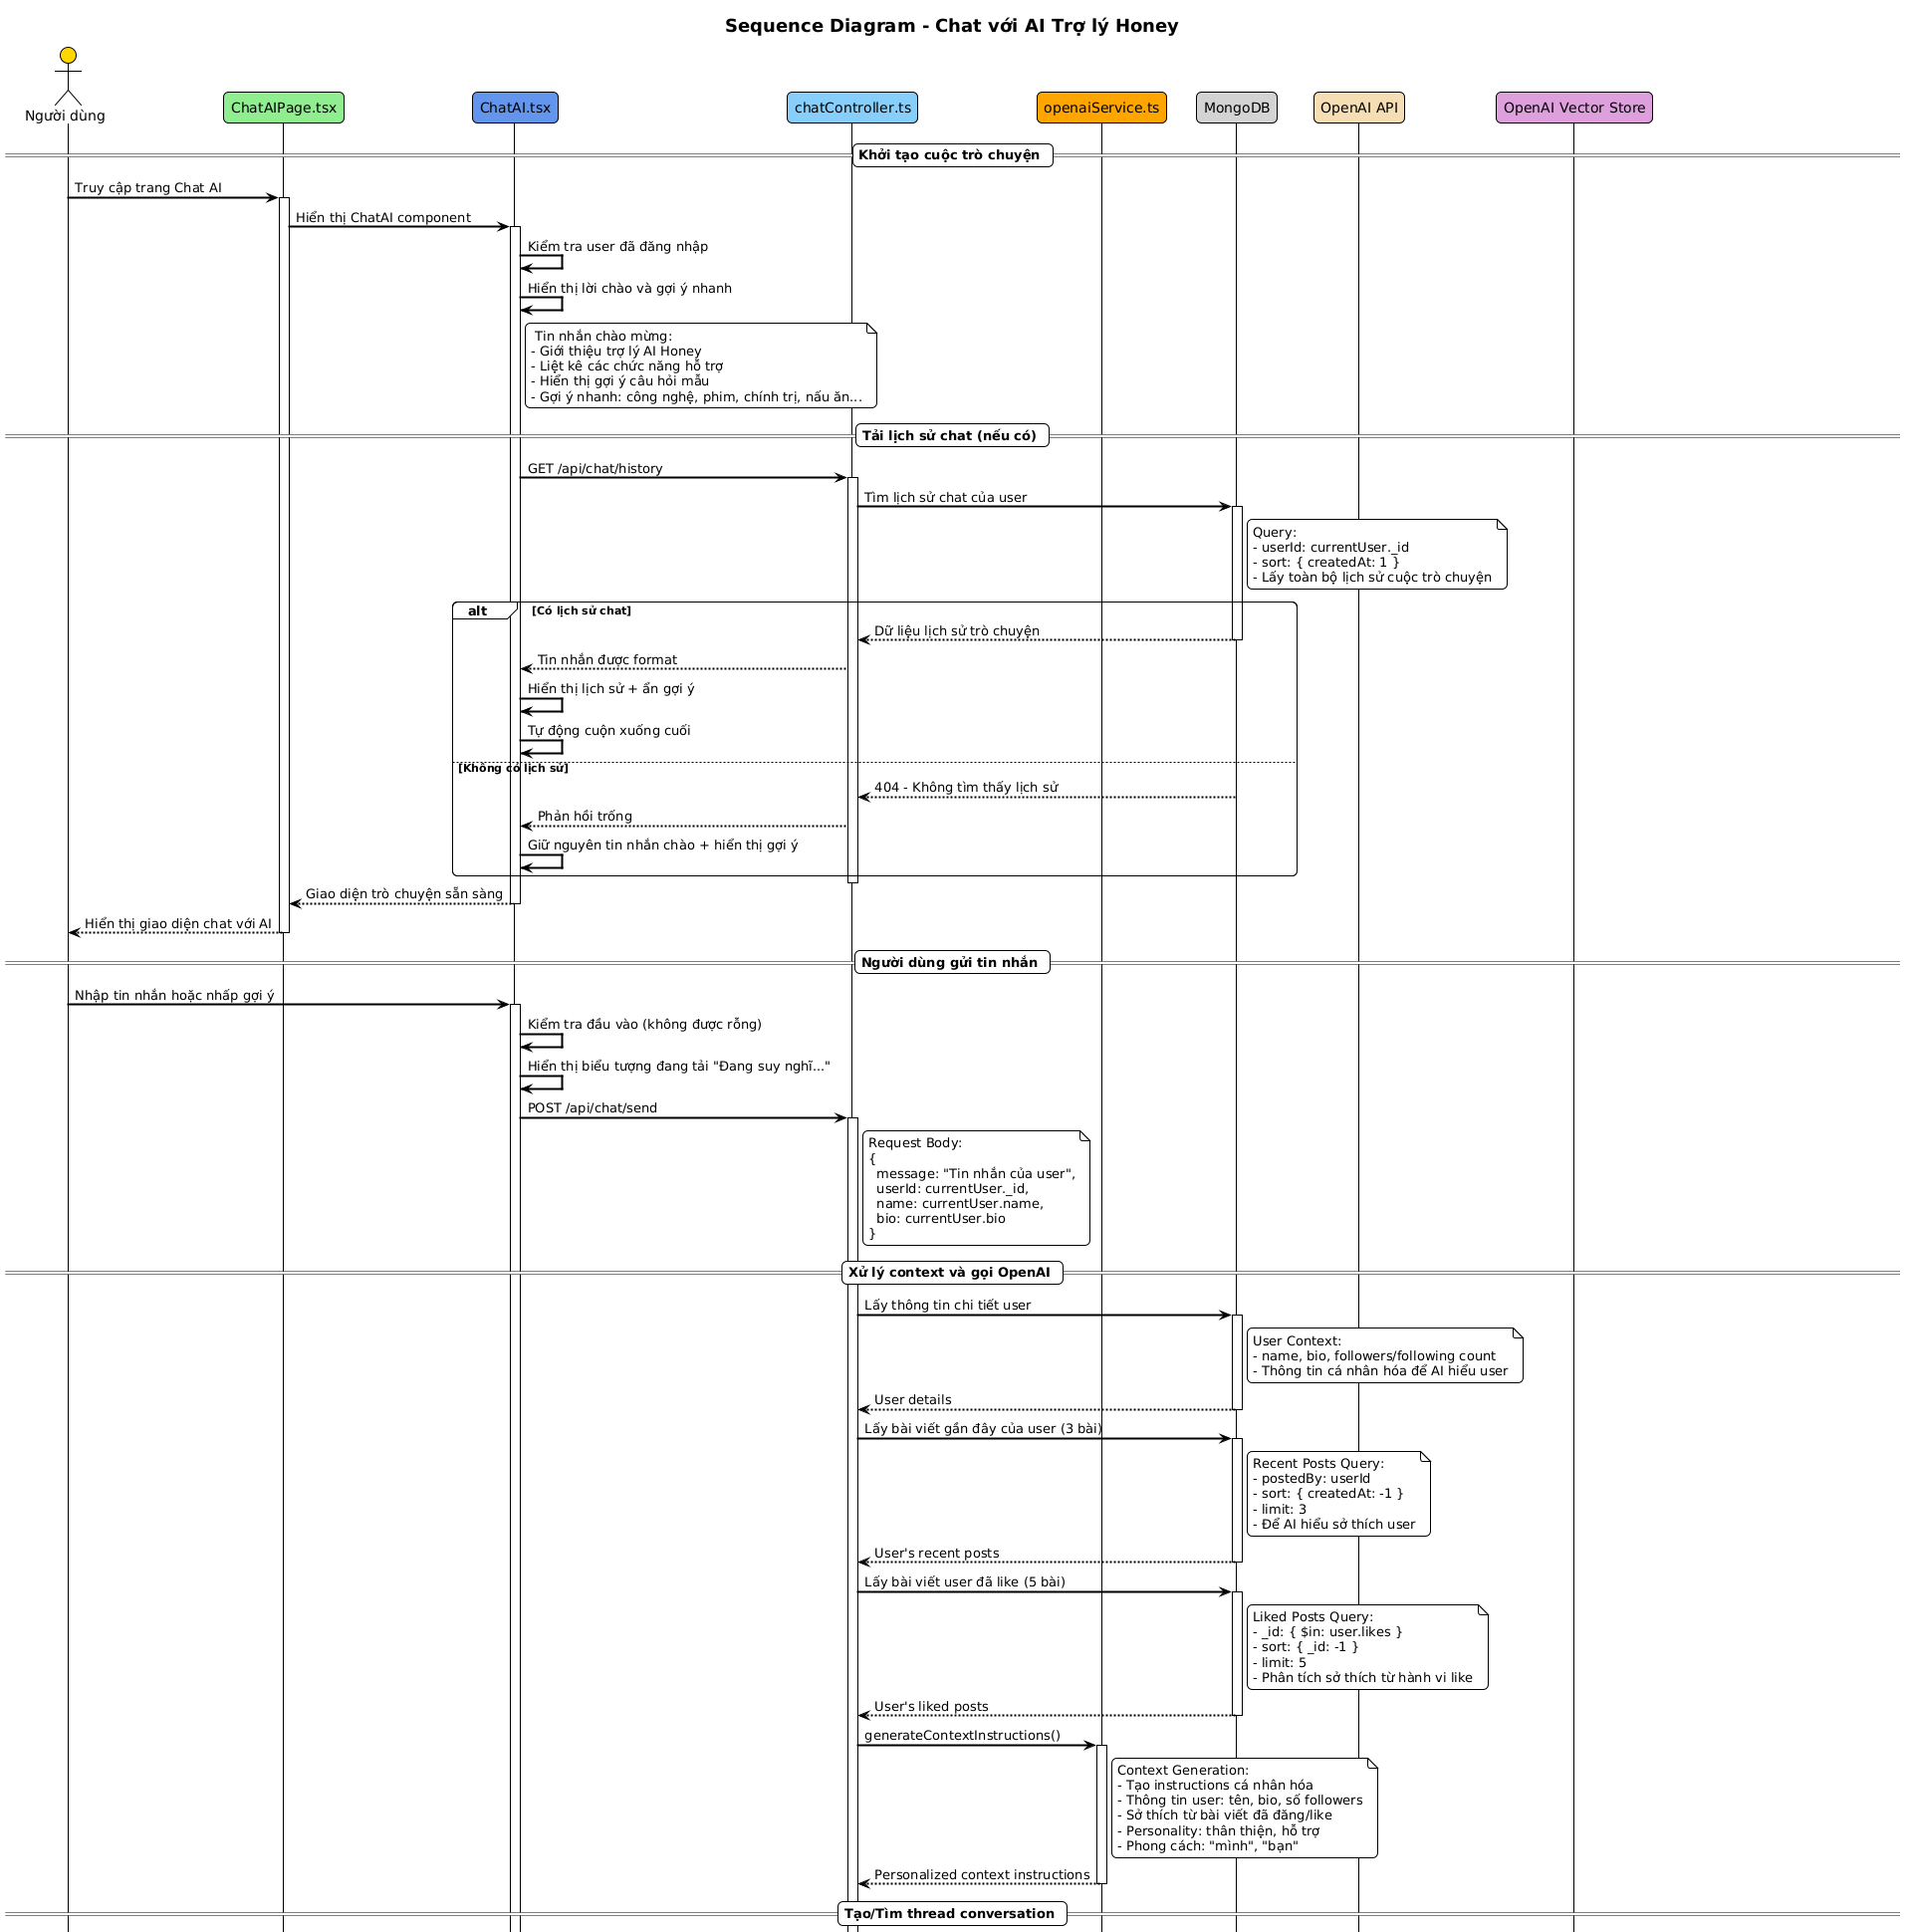
\includegraphics[width=1\textwidth]{image/sequence/chat-ai.png}
%     \caption{Hình ảnh Chat AI}
%     \label{fig:chat_ai}
% \end{figure}


% \begin{figure}[H]
%     \centering
%     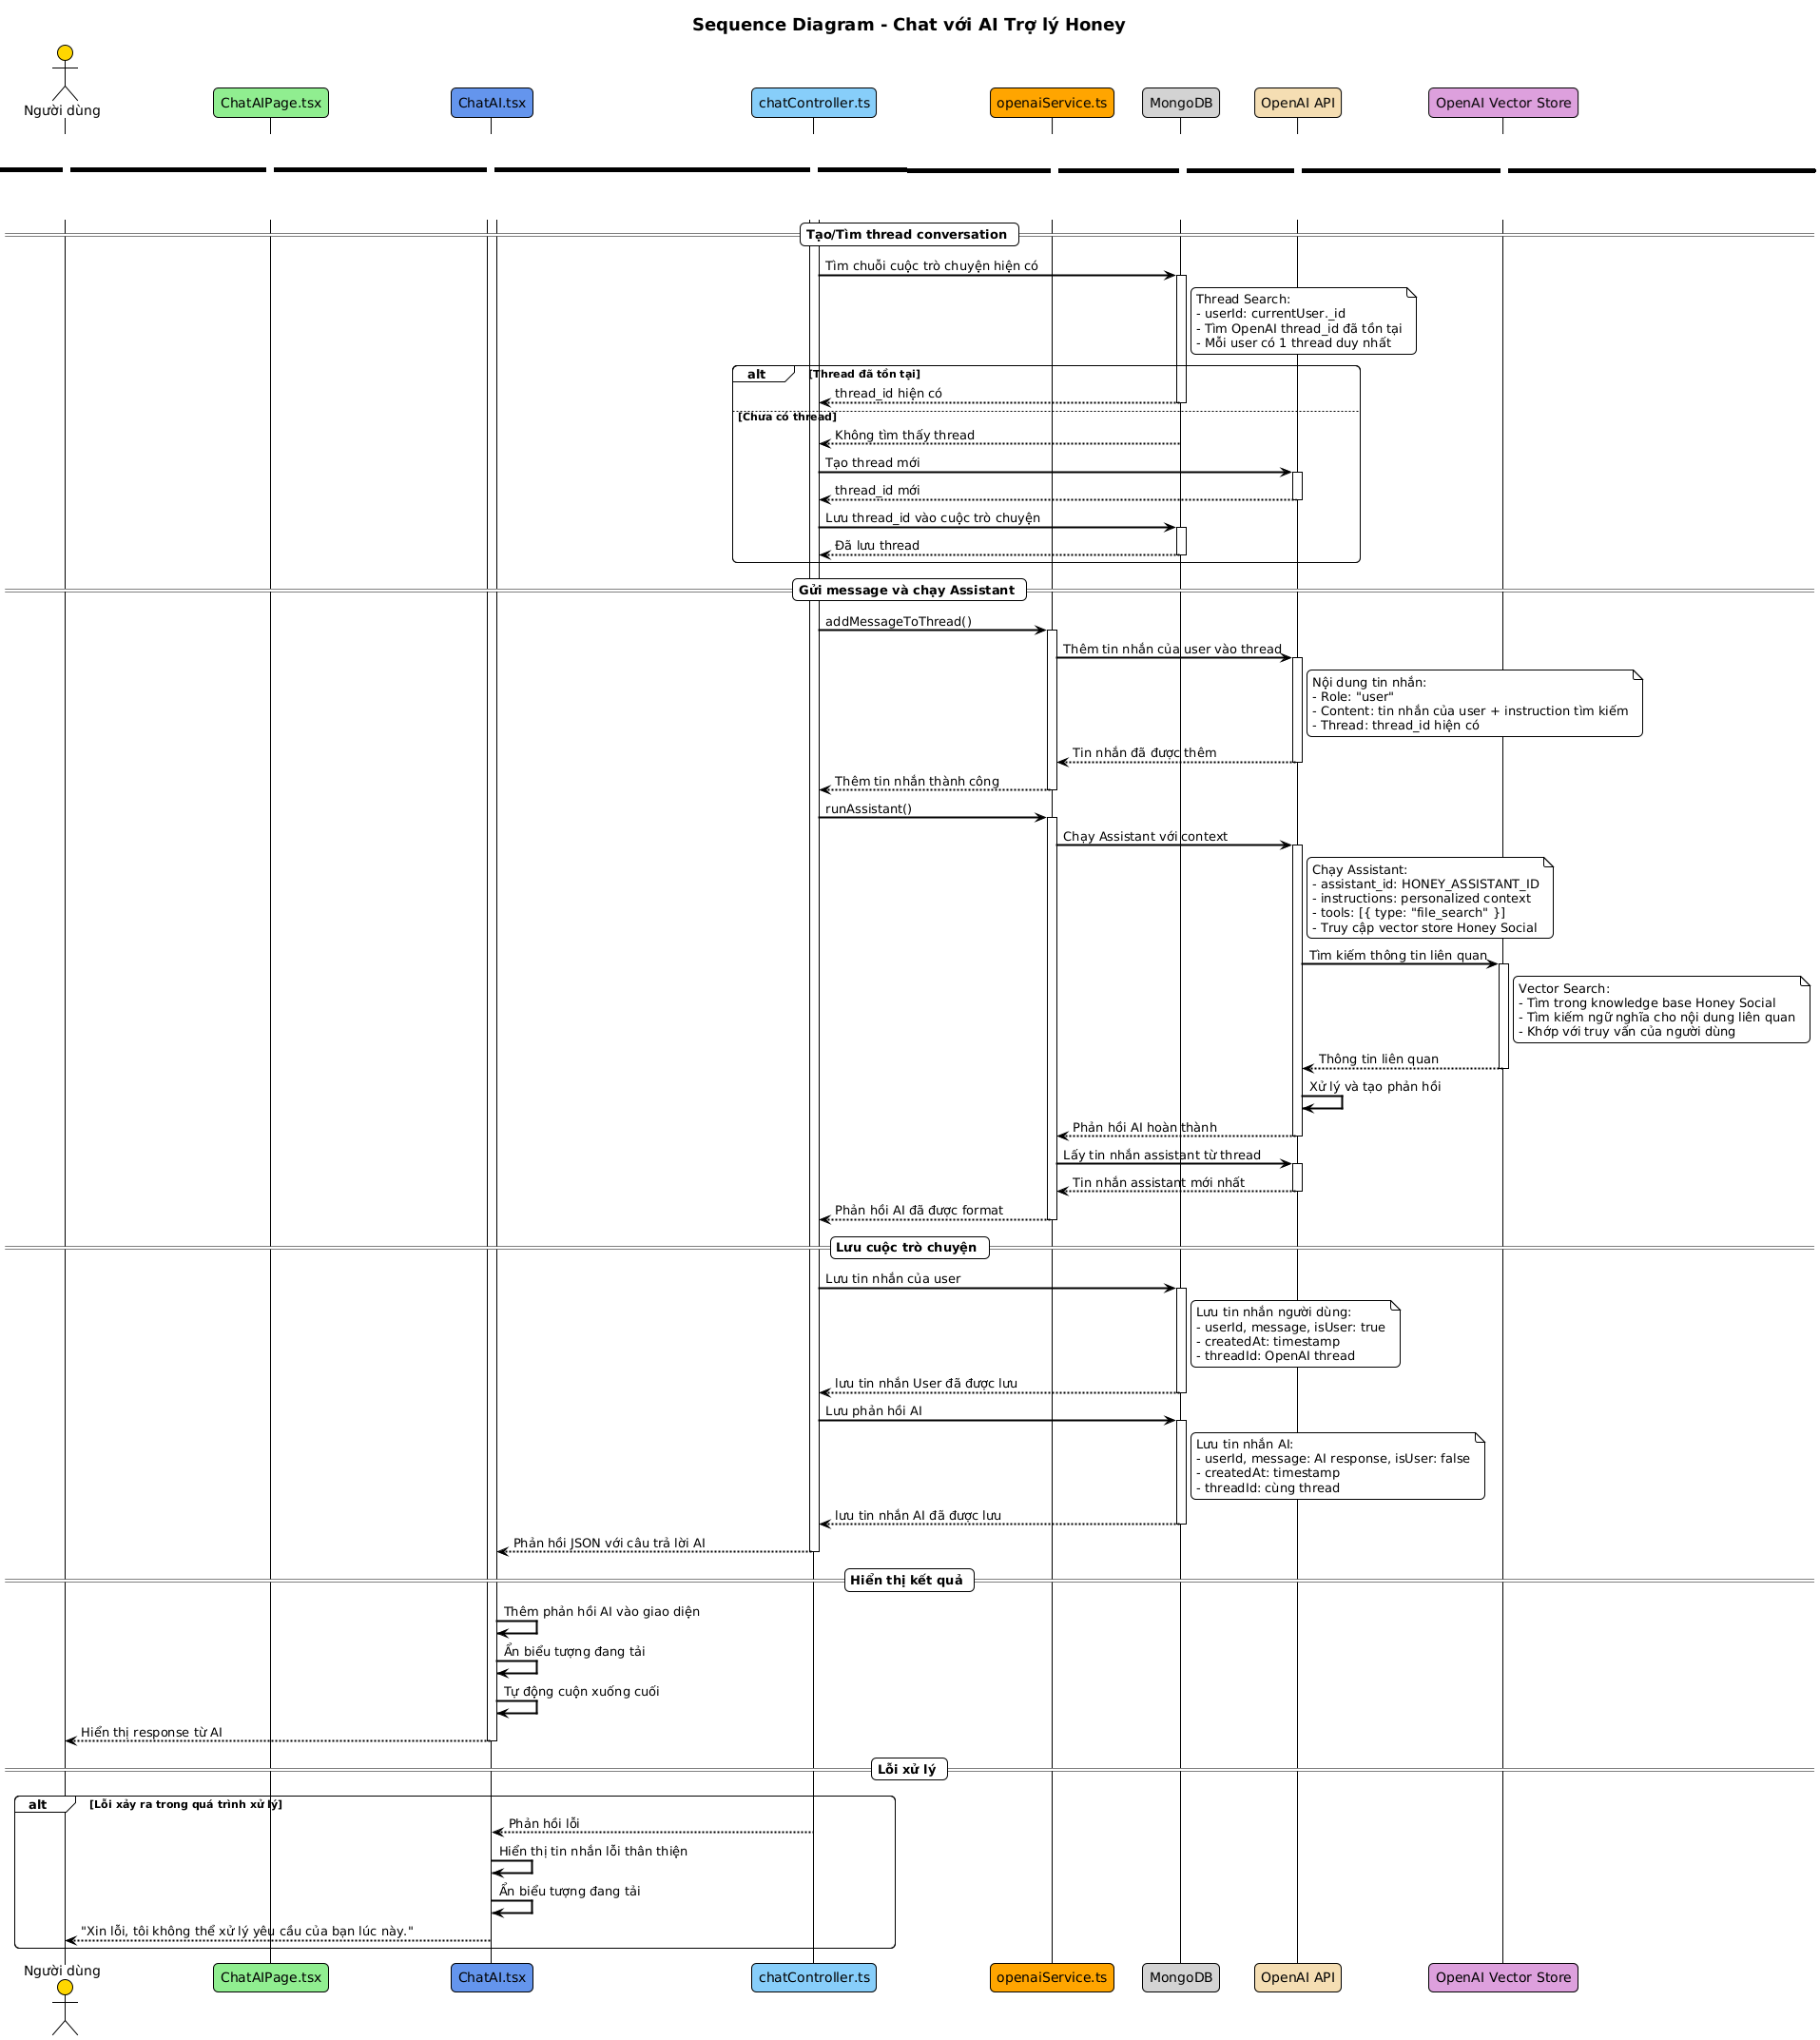
\includegraphics[width=1\textwidth]{image/sequence/chat-ai2.png}
%     \caption{Hình ảnh Chat AI 2}
%     \label{fig:chat_ai2}
% \end{figure}


% \begin{figure}[H]
%     \centering
%     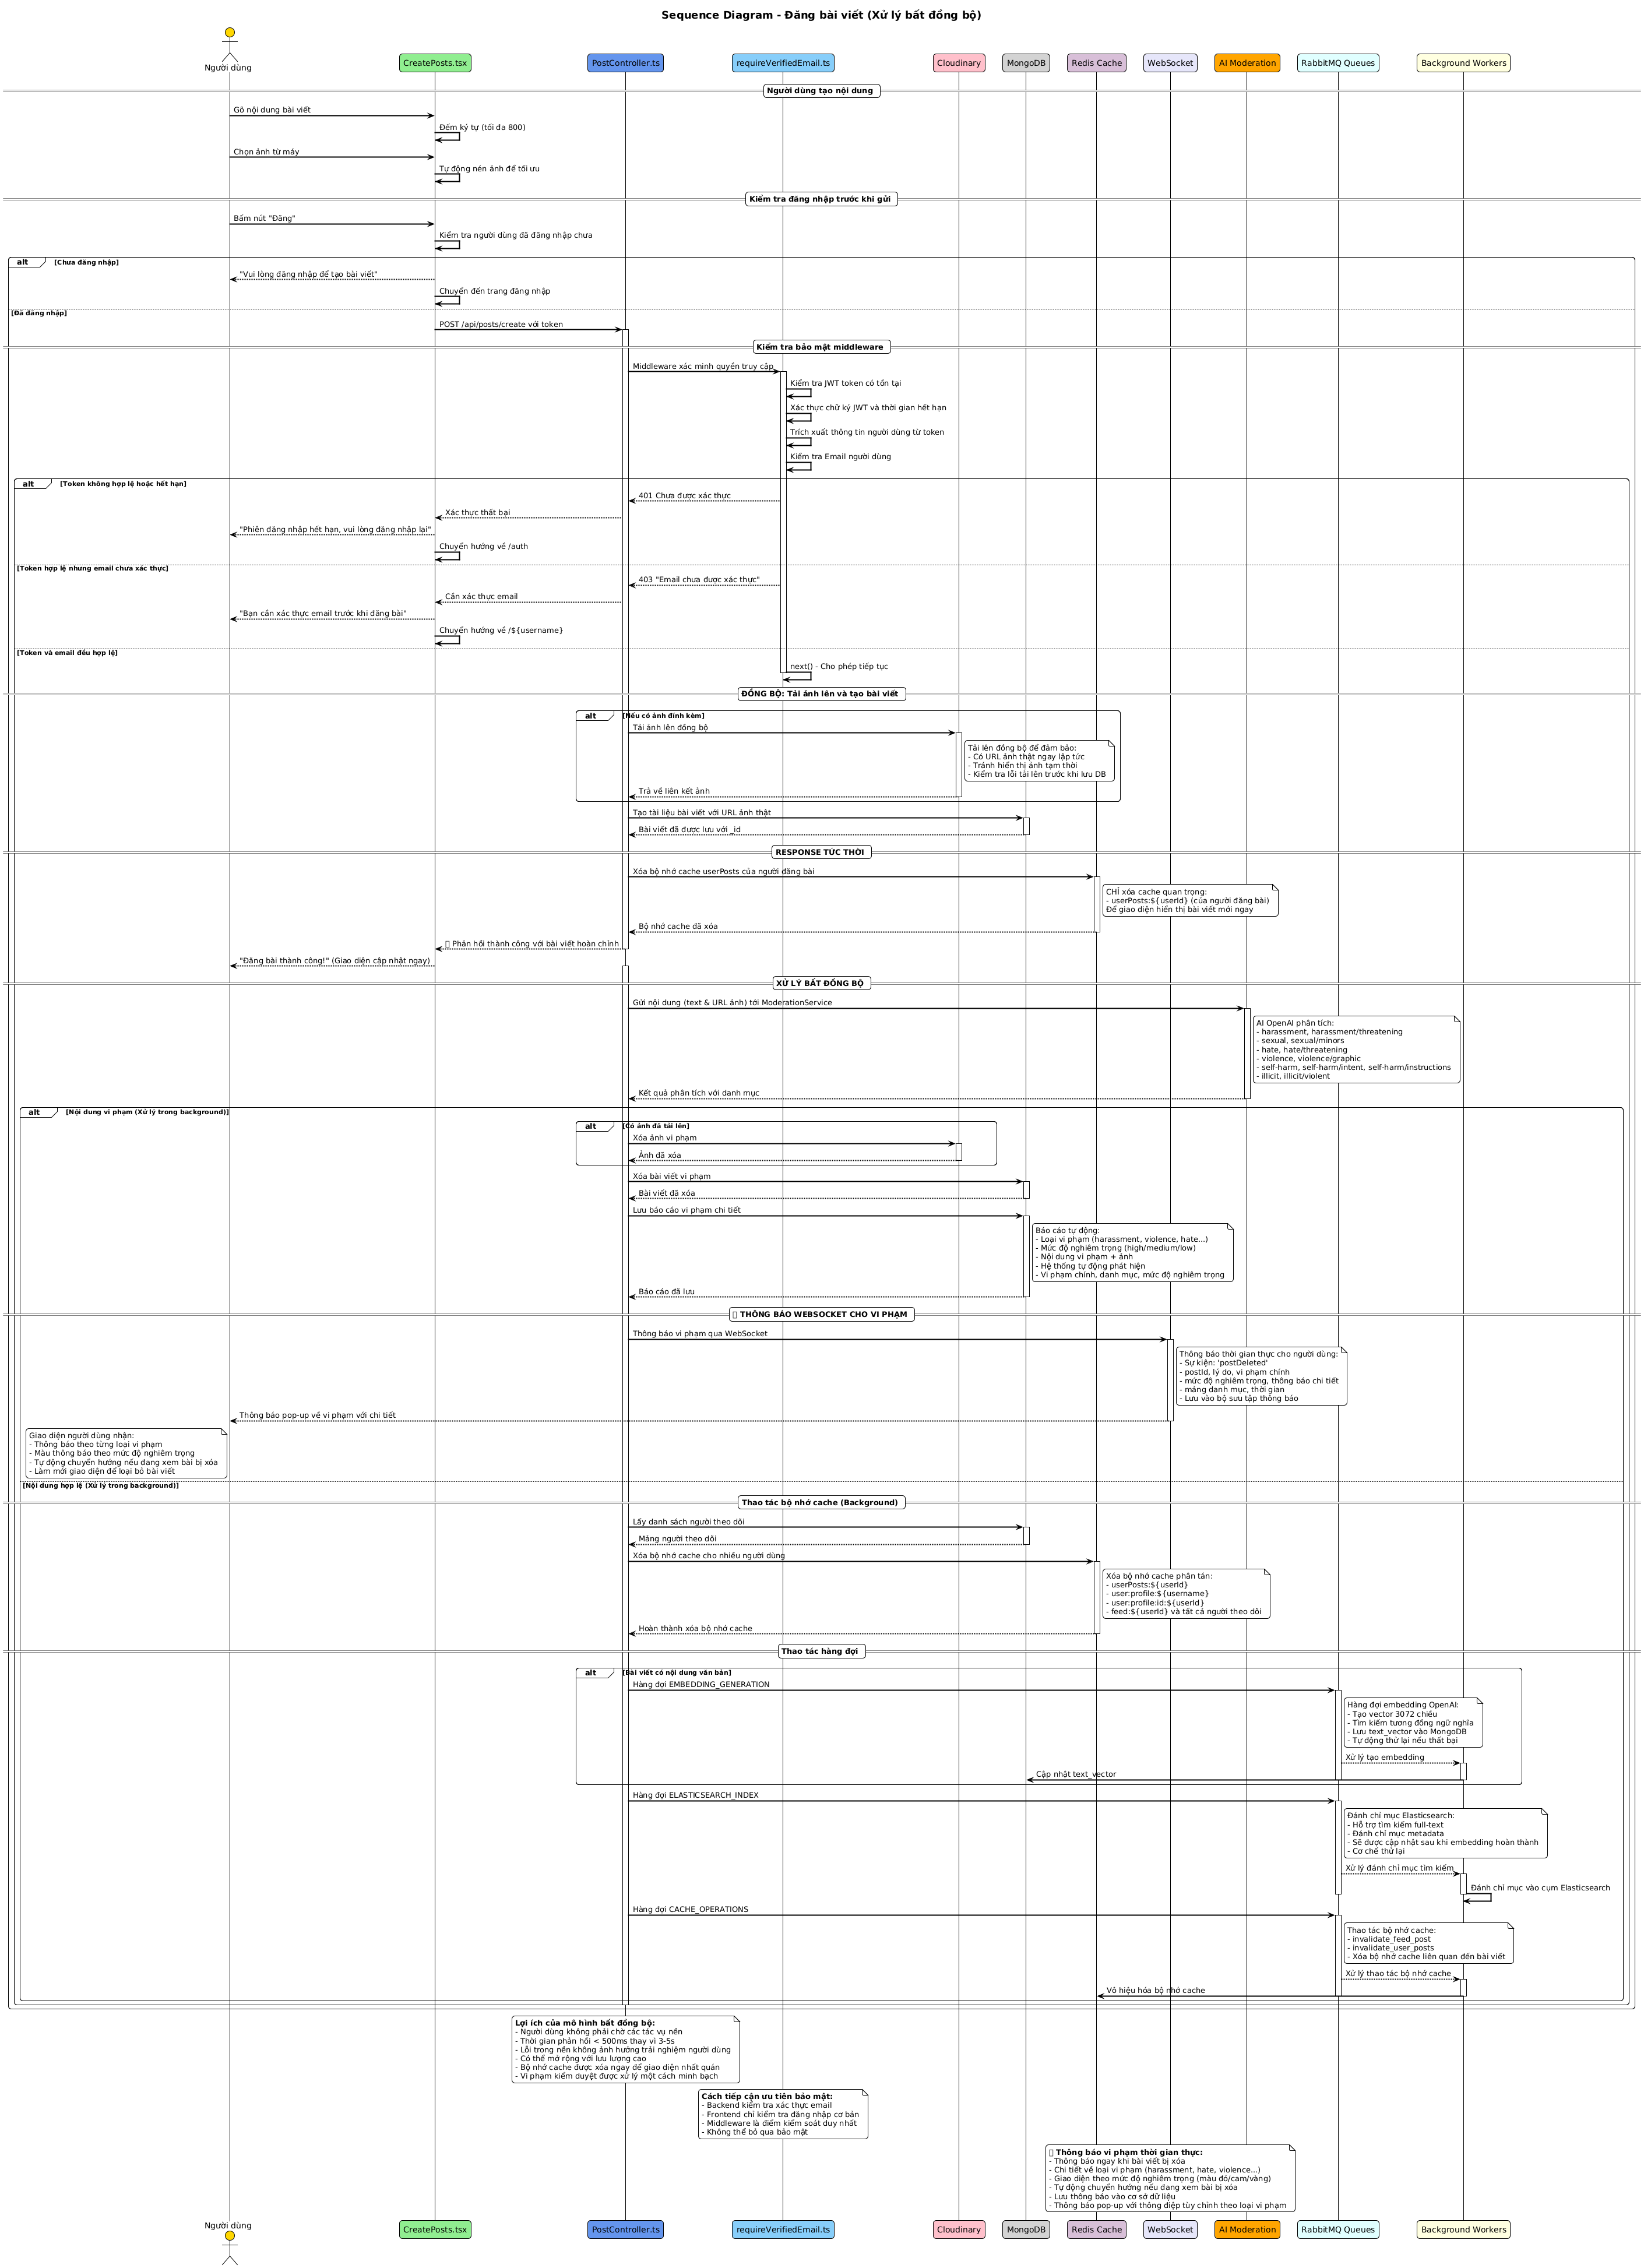
\includegraphics[width=1\textwidth]{image/sequence/dang-bai-viet.png}
%     \caption{Hình ảnh Đăng bài viết}
%     \label{fig:dang_bai_viet}
% \end{figure}

% \begin{figure}[H]
%     \centering
%     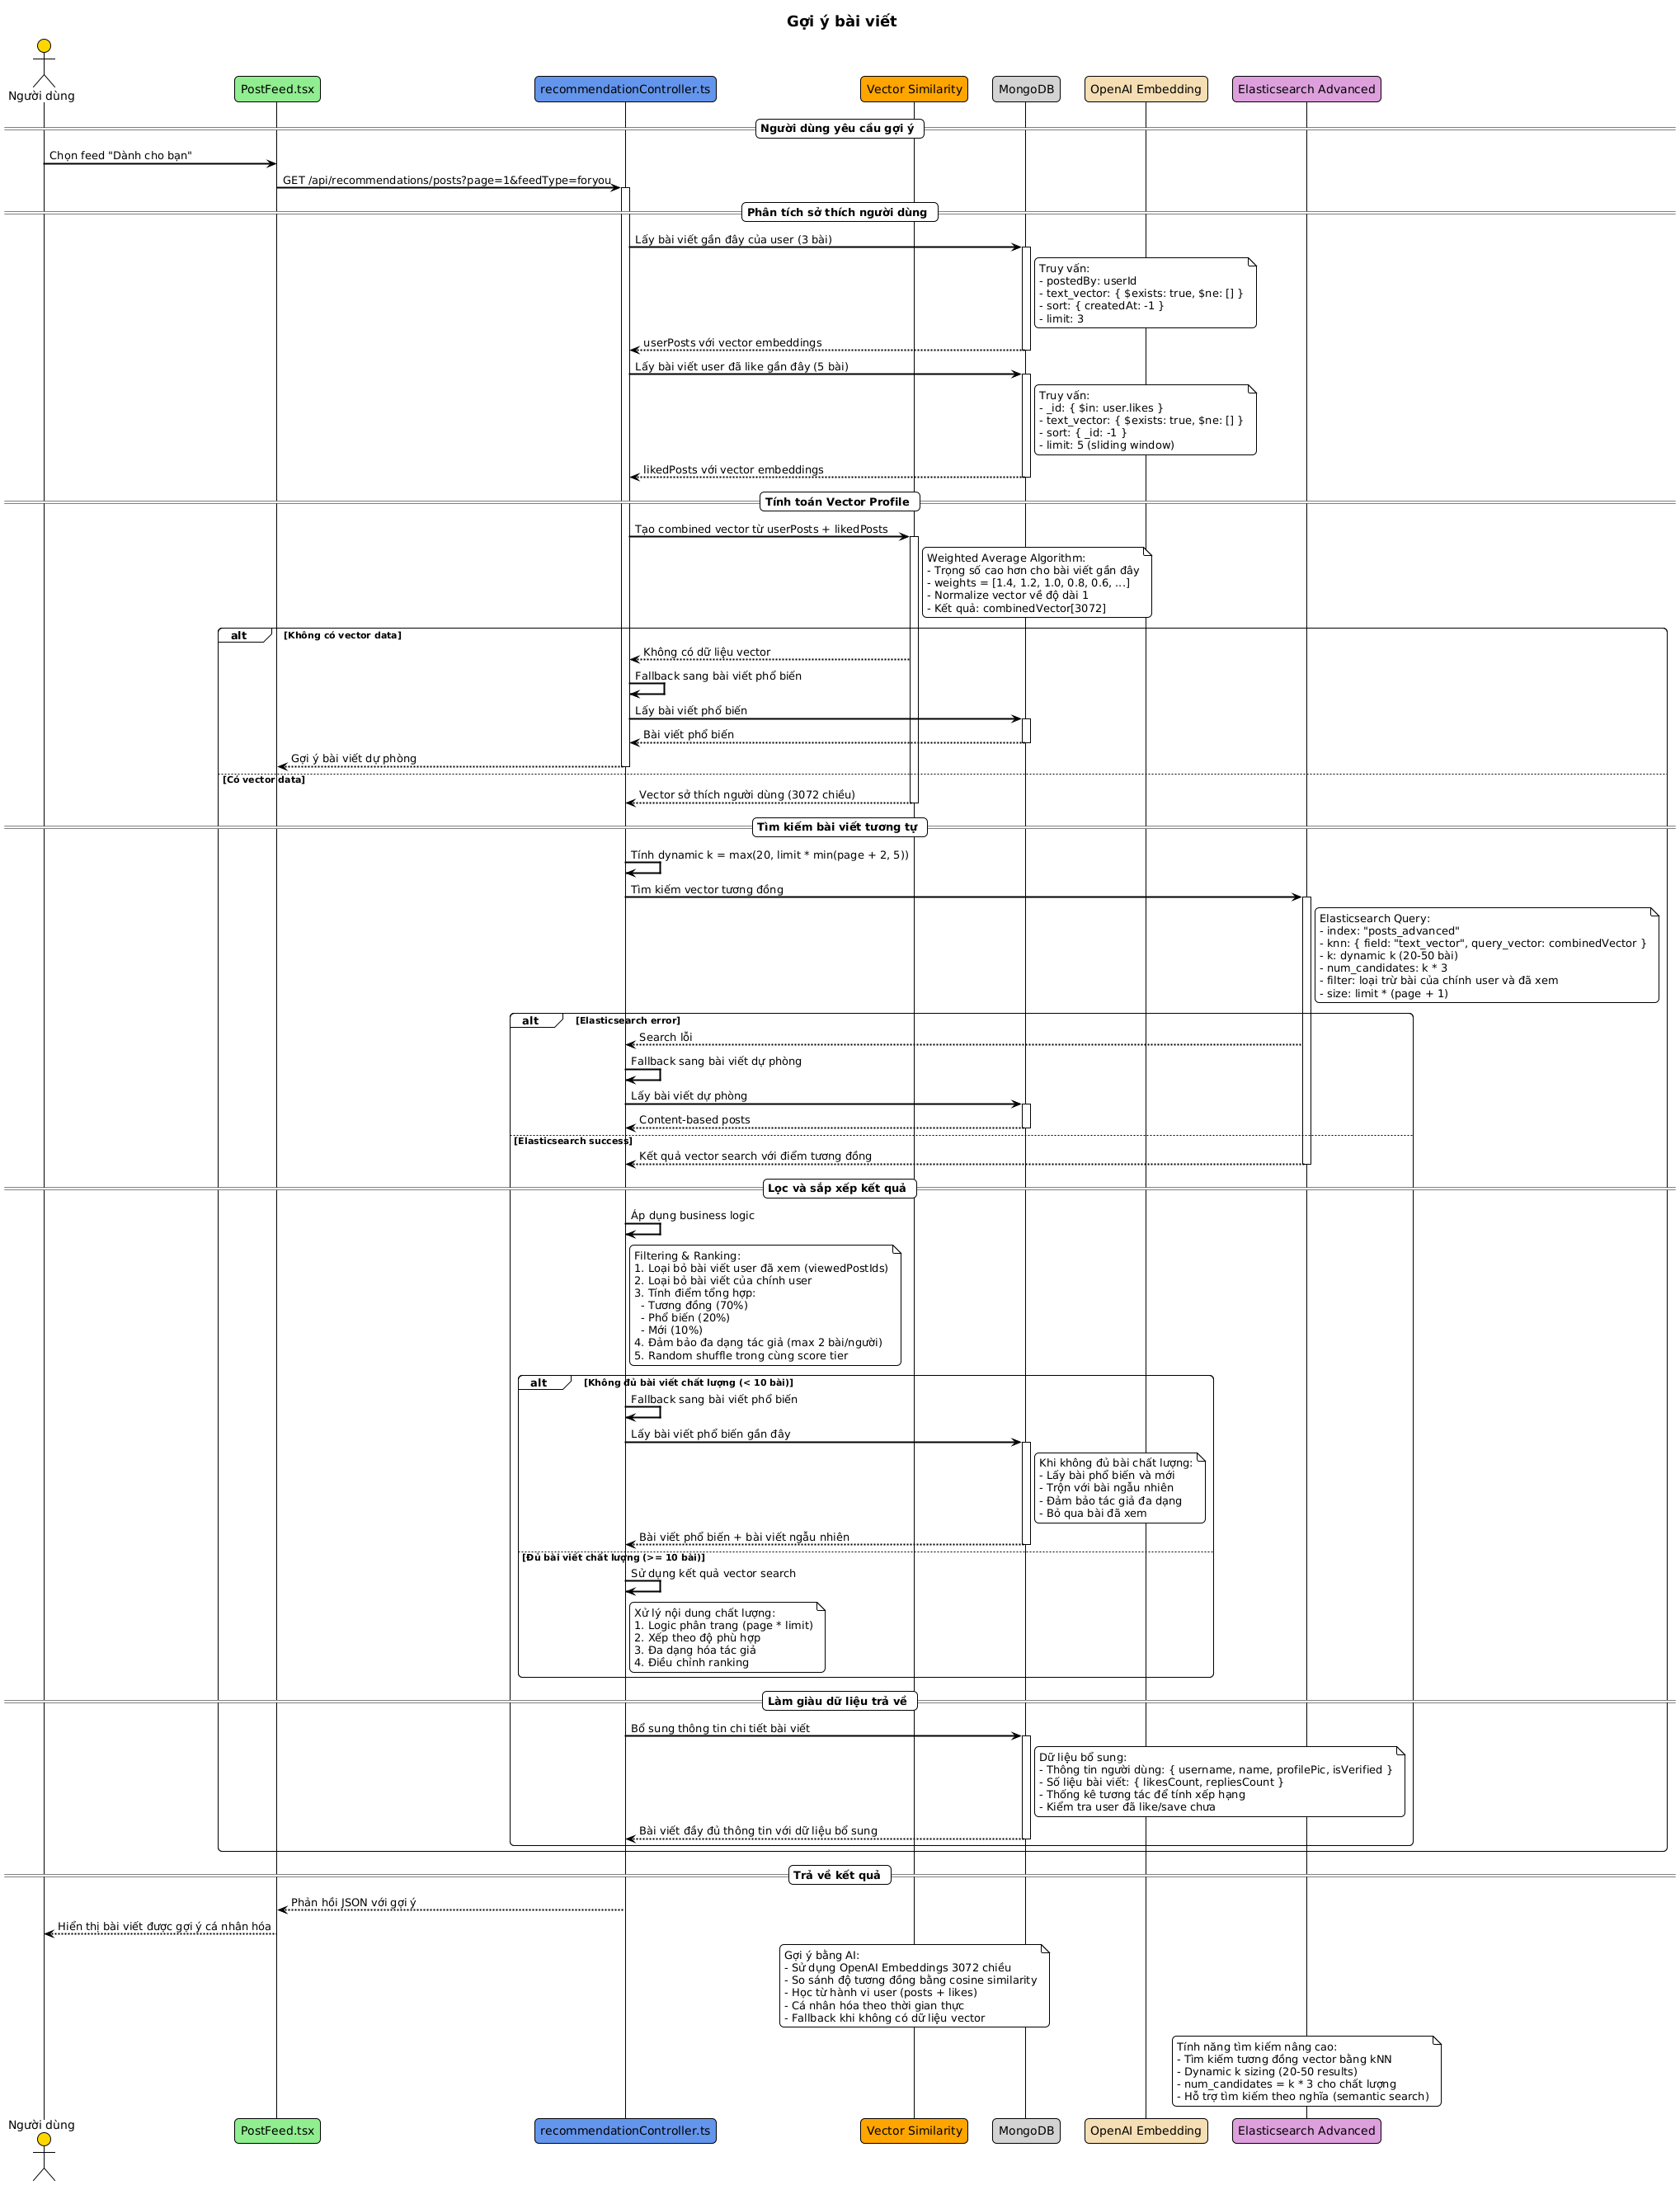
\includegraphics[width=1\textwidth]{image/sequence/goi-y-bai-viet.png}
%     \caption{Hình ảnh Gợi ý bài viết}
%     \label{fig:goi_y_bai_viet}
% \end{figure}

% \begin{figure}[H]
%     \centering
%     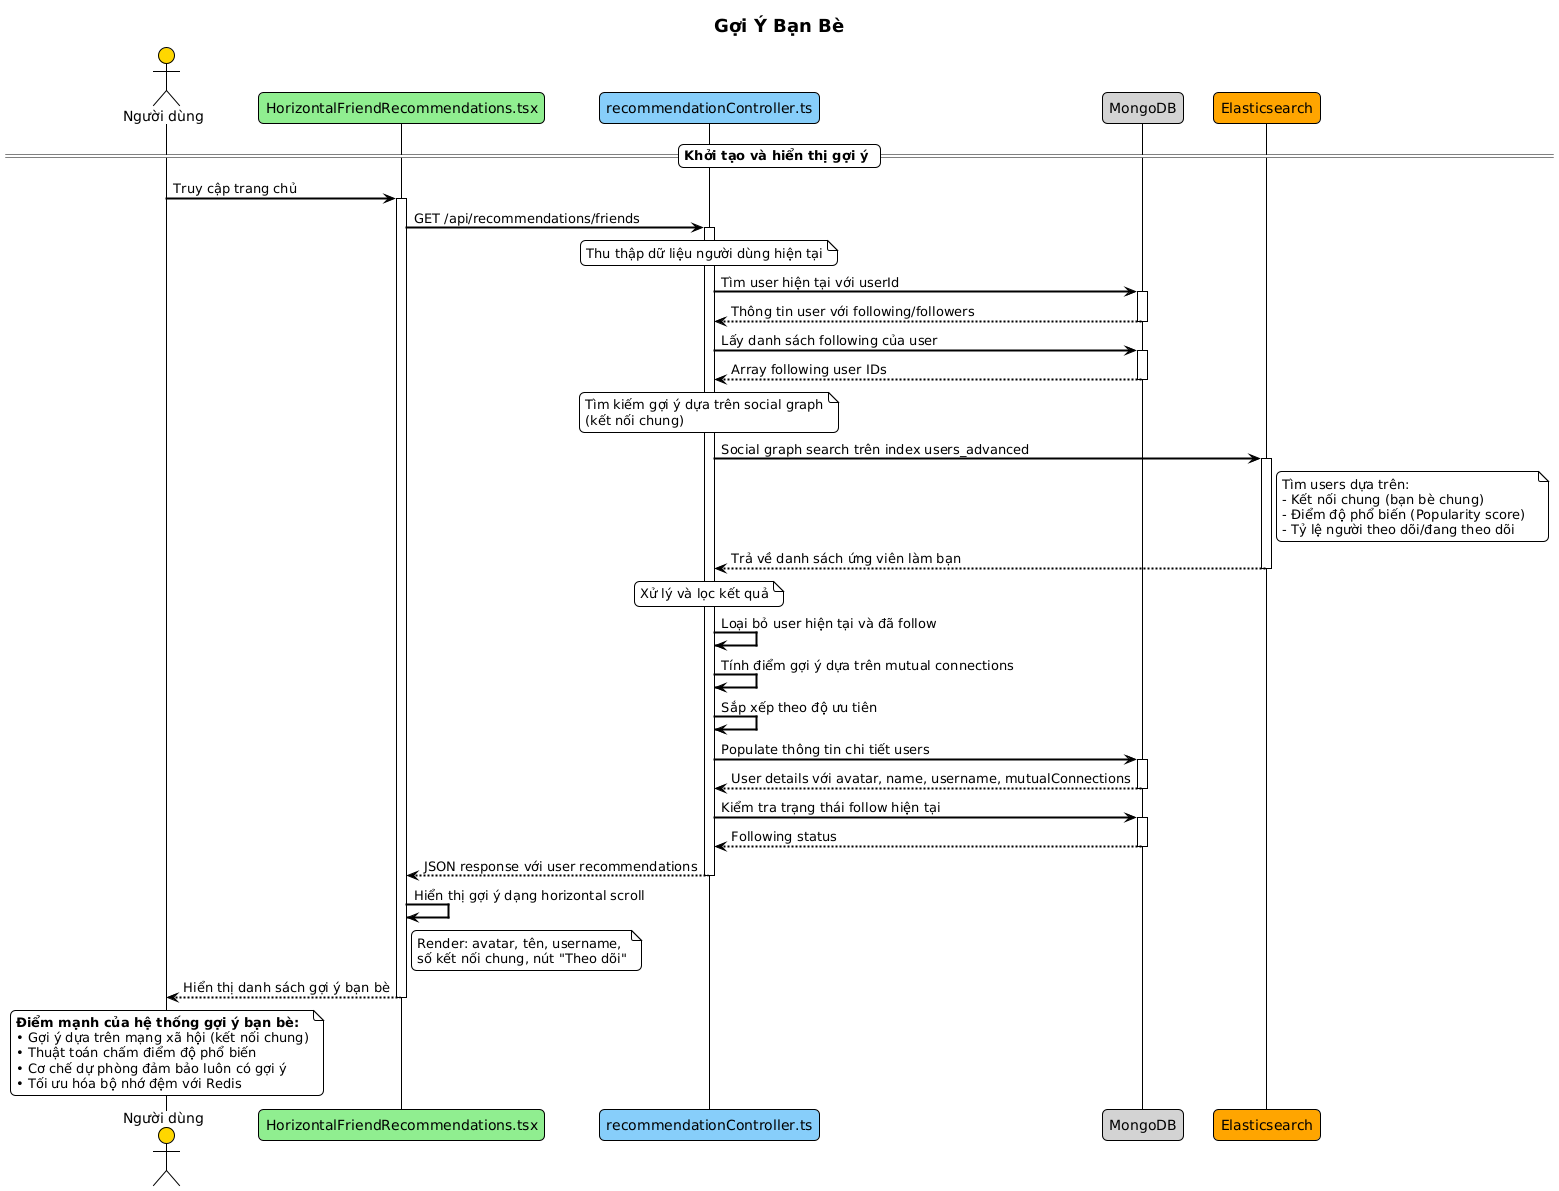
\includegraphics[width=1\textwidth]{image/sequence/goi-y-ban-be.png}
%     \caption{Hình ảnh Gợi ý bạn bè}
%     \label{fig:goi_y_ban_be}
% \end{figure}


% \begin{figure}[H]
%     \centering
%     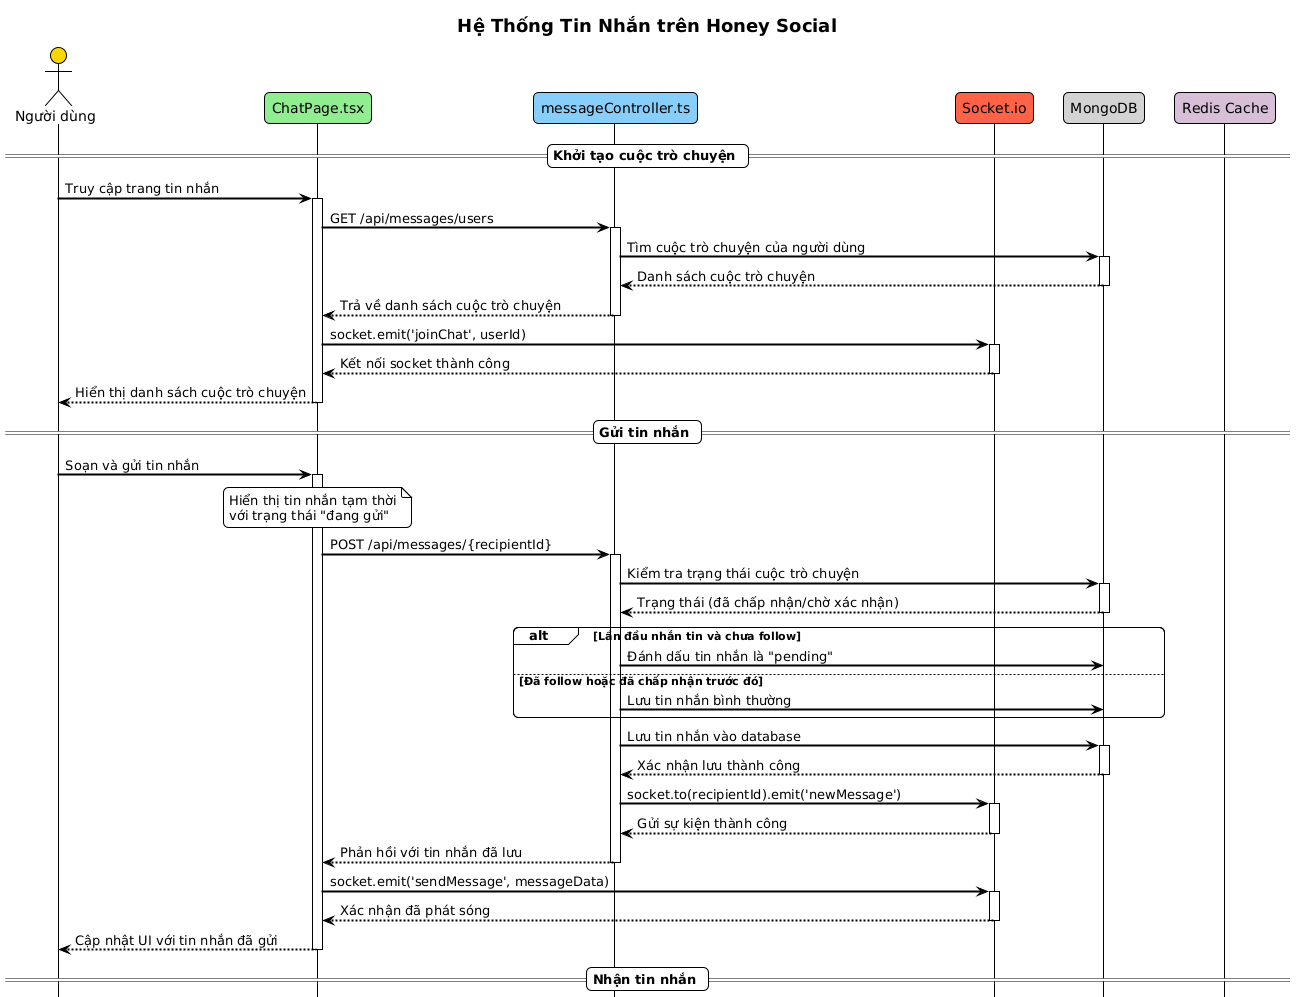
\includegraphics[width=1\textwidth]{image/sequence/message1.png}
%     \caption{Hình ảnh Hệ thống tin nhắn trên Honey Social}
%     \label{fig:message1}
% \end{figure}


% \begin{figure}[H]
%     \centering
%     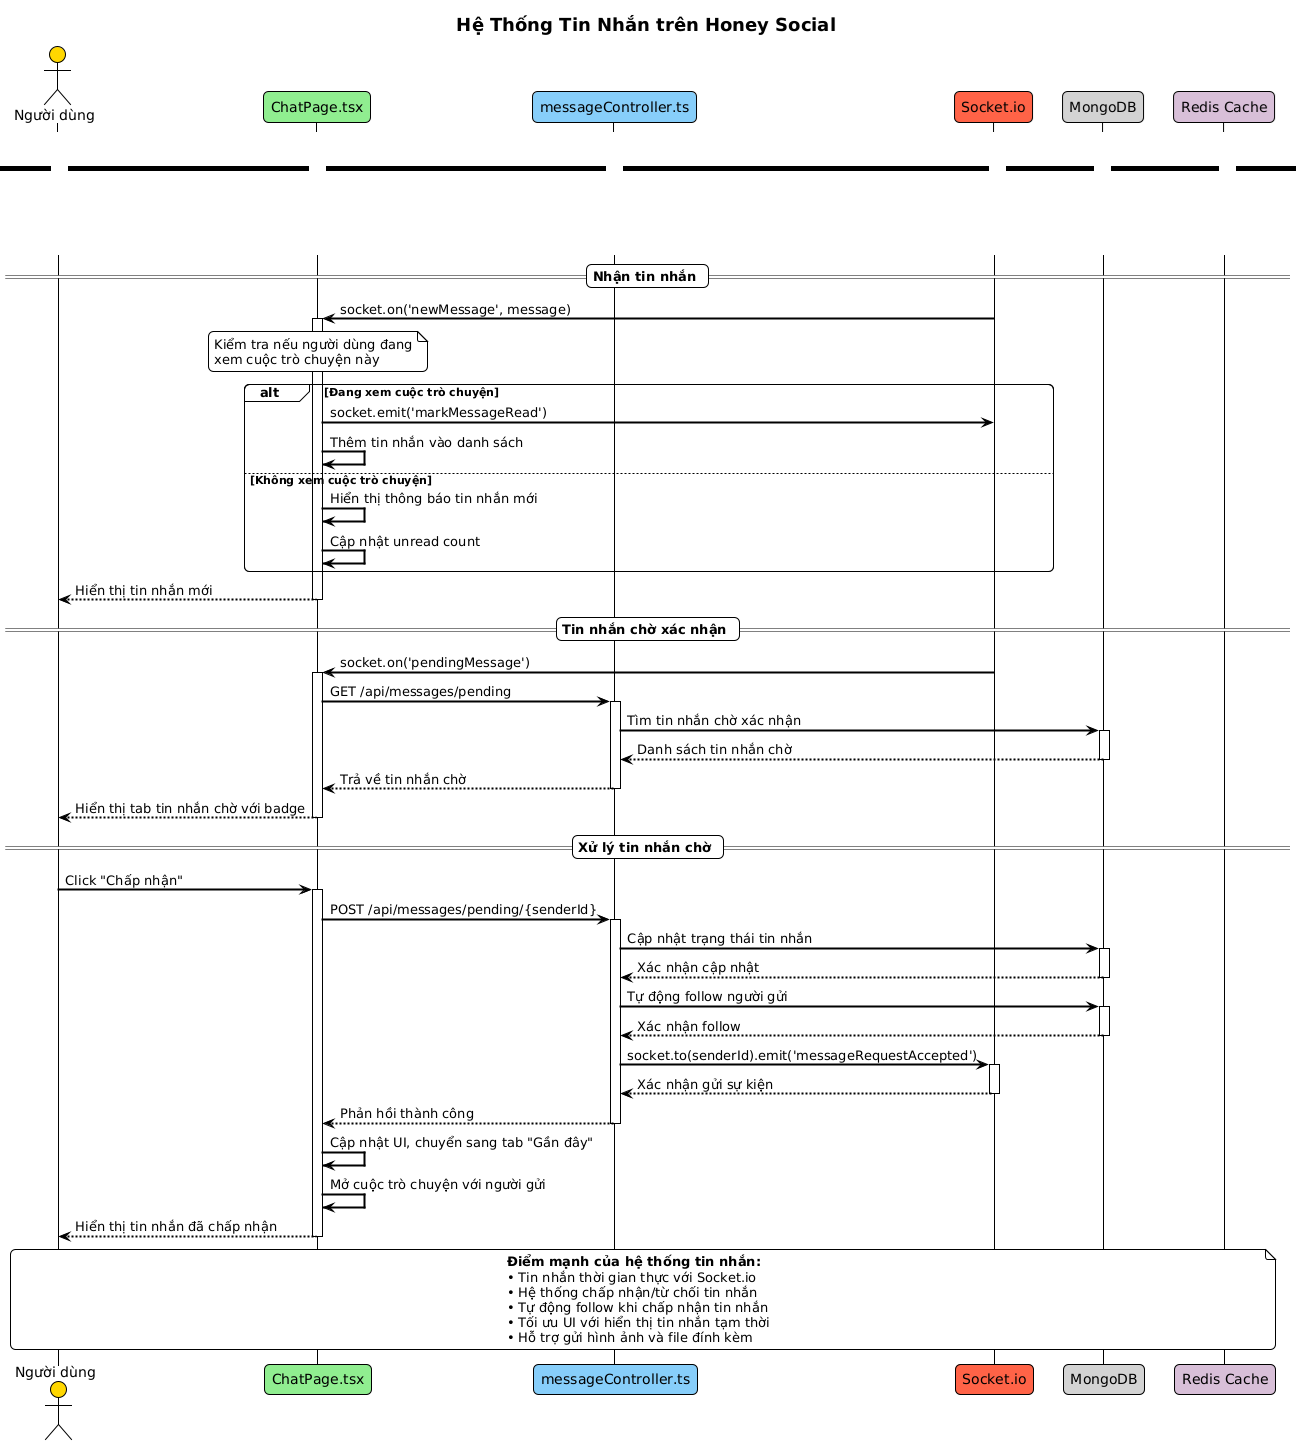
\includegraphics[width=1\textwidth]{image/sequence/message2.png}
%     \caption{Hình ảnh Hệ thống tin nhắn trên Honey Social 2}
%     \label{fig:message}
% \end{figure}




% \begin{figure}[H]
%     \centering
%     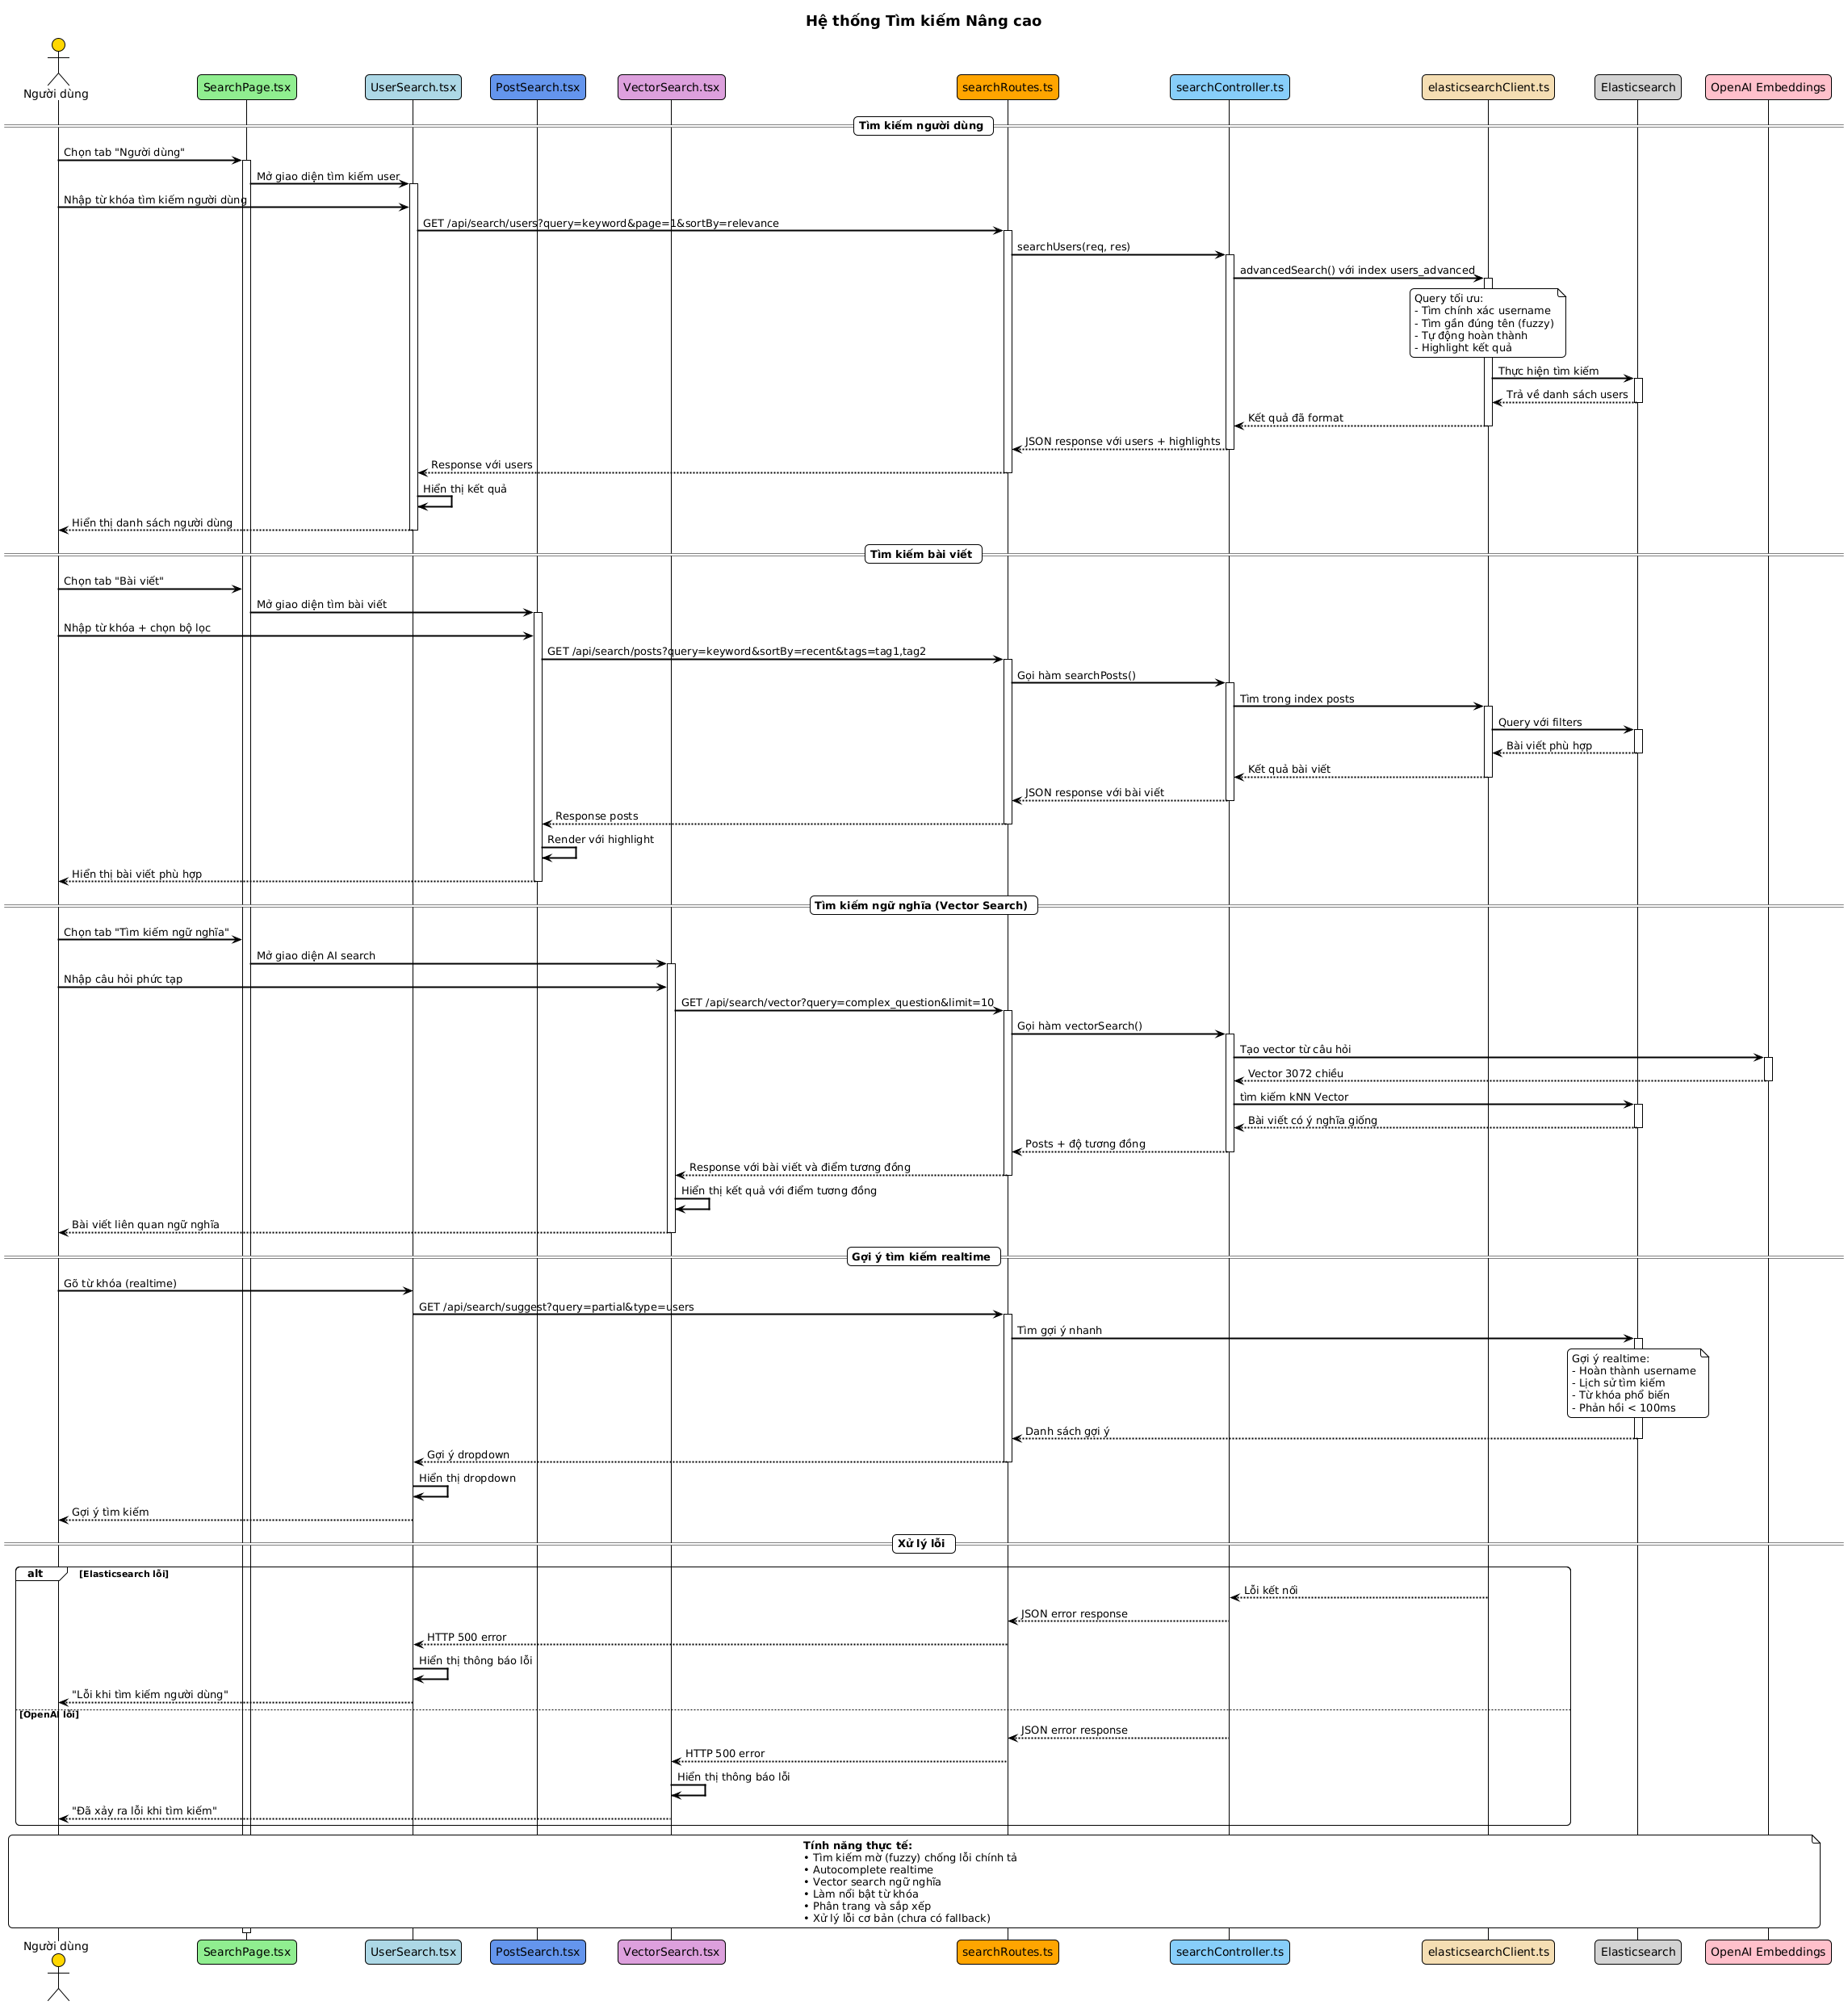
\includegraphics[width=1\textwidth]{image/sequence/tim-kiem-nang-cao.png}
%     \caption{Hình ảnh Tìm kiếm nâng cao}
%     \label{fig:tim_kiem_nang_cao}
% \end{figure}

\newpage
\section{\textbf{THIẾT KẾ HỆ THỐNG}}

\subsection{Tổng quan hệ thống}

\begin{figure}[H]
	\centering
	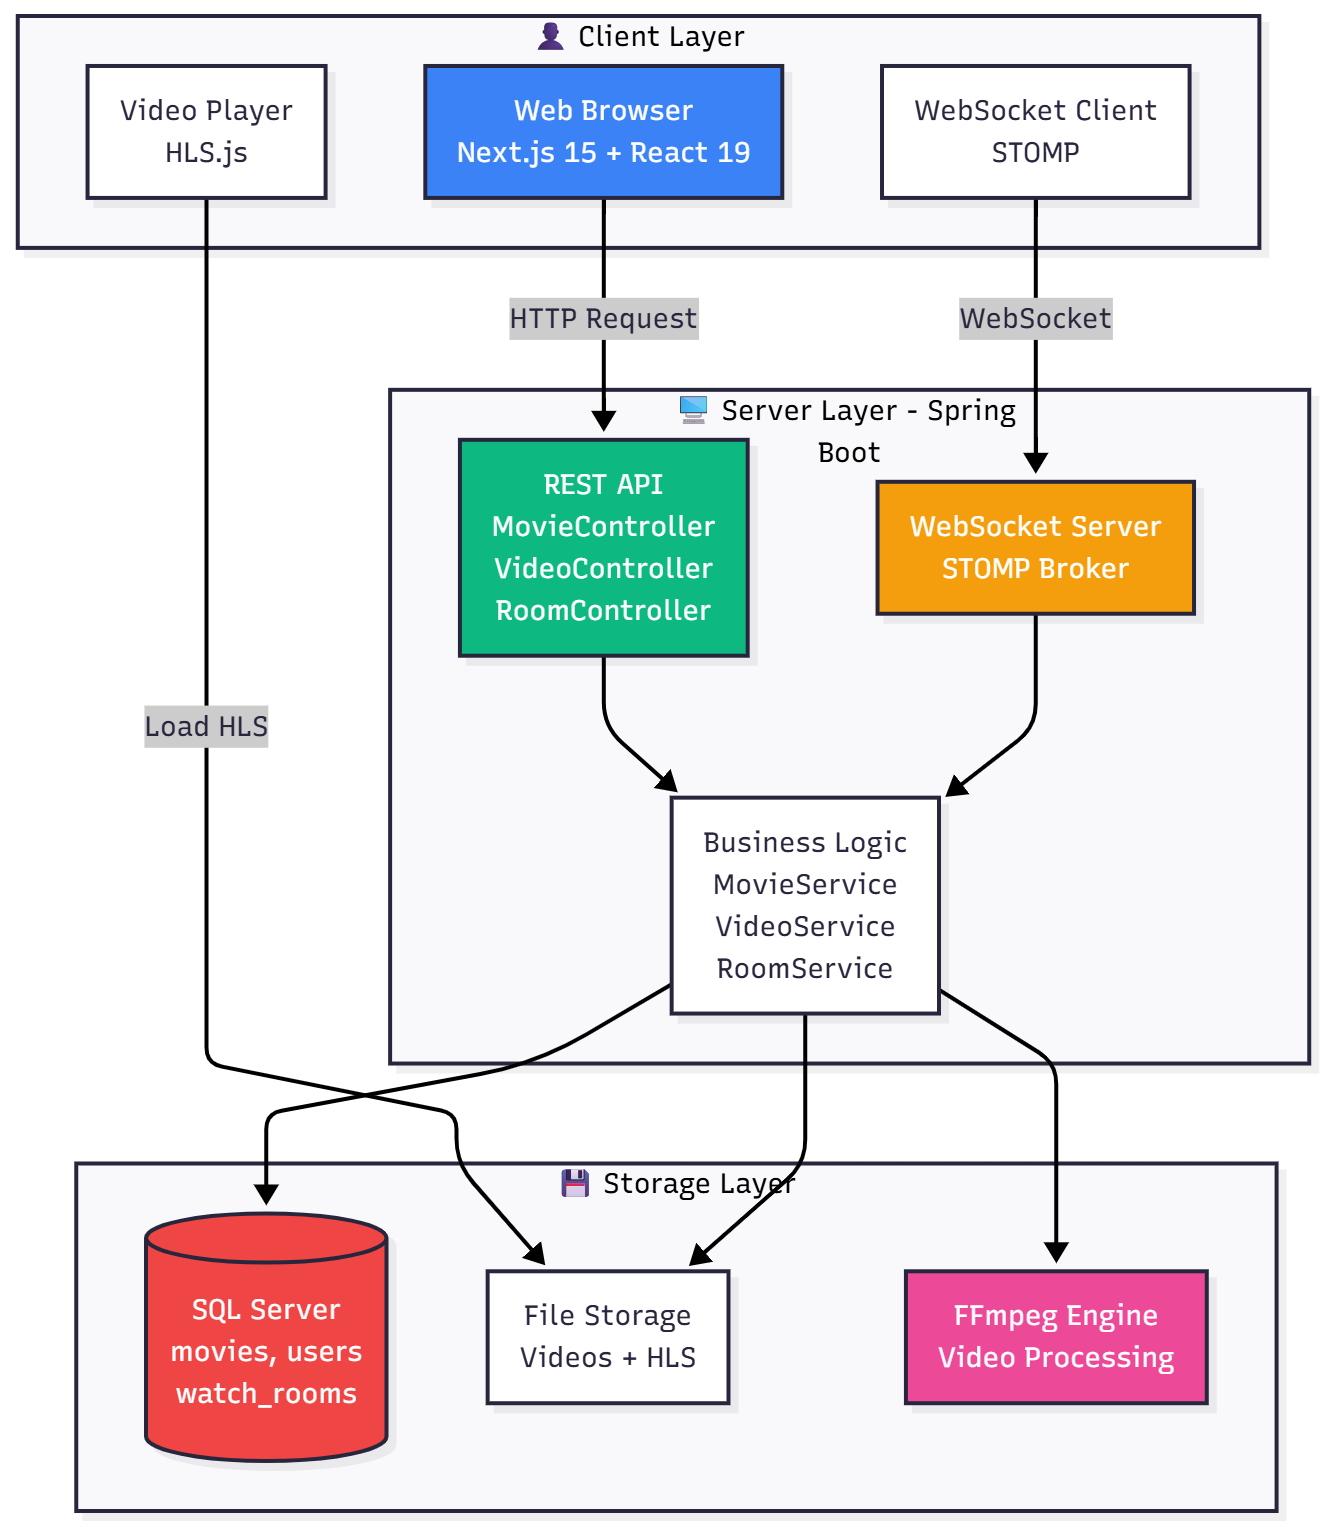
\includegraphics[width=1\textwidth]{image/mermaid/tongquahethong.png}
	\caption{Tổng quan hệ thống NicePhim}
	\label{fig:tongquahethong}
\end{figure}

\subsection{Luồng xử lý video}

\begin{figure}[H]
	\centering
	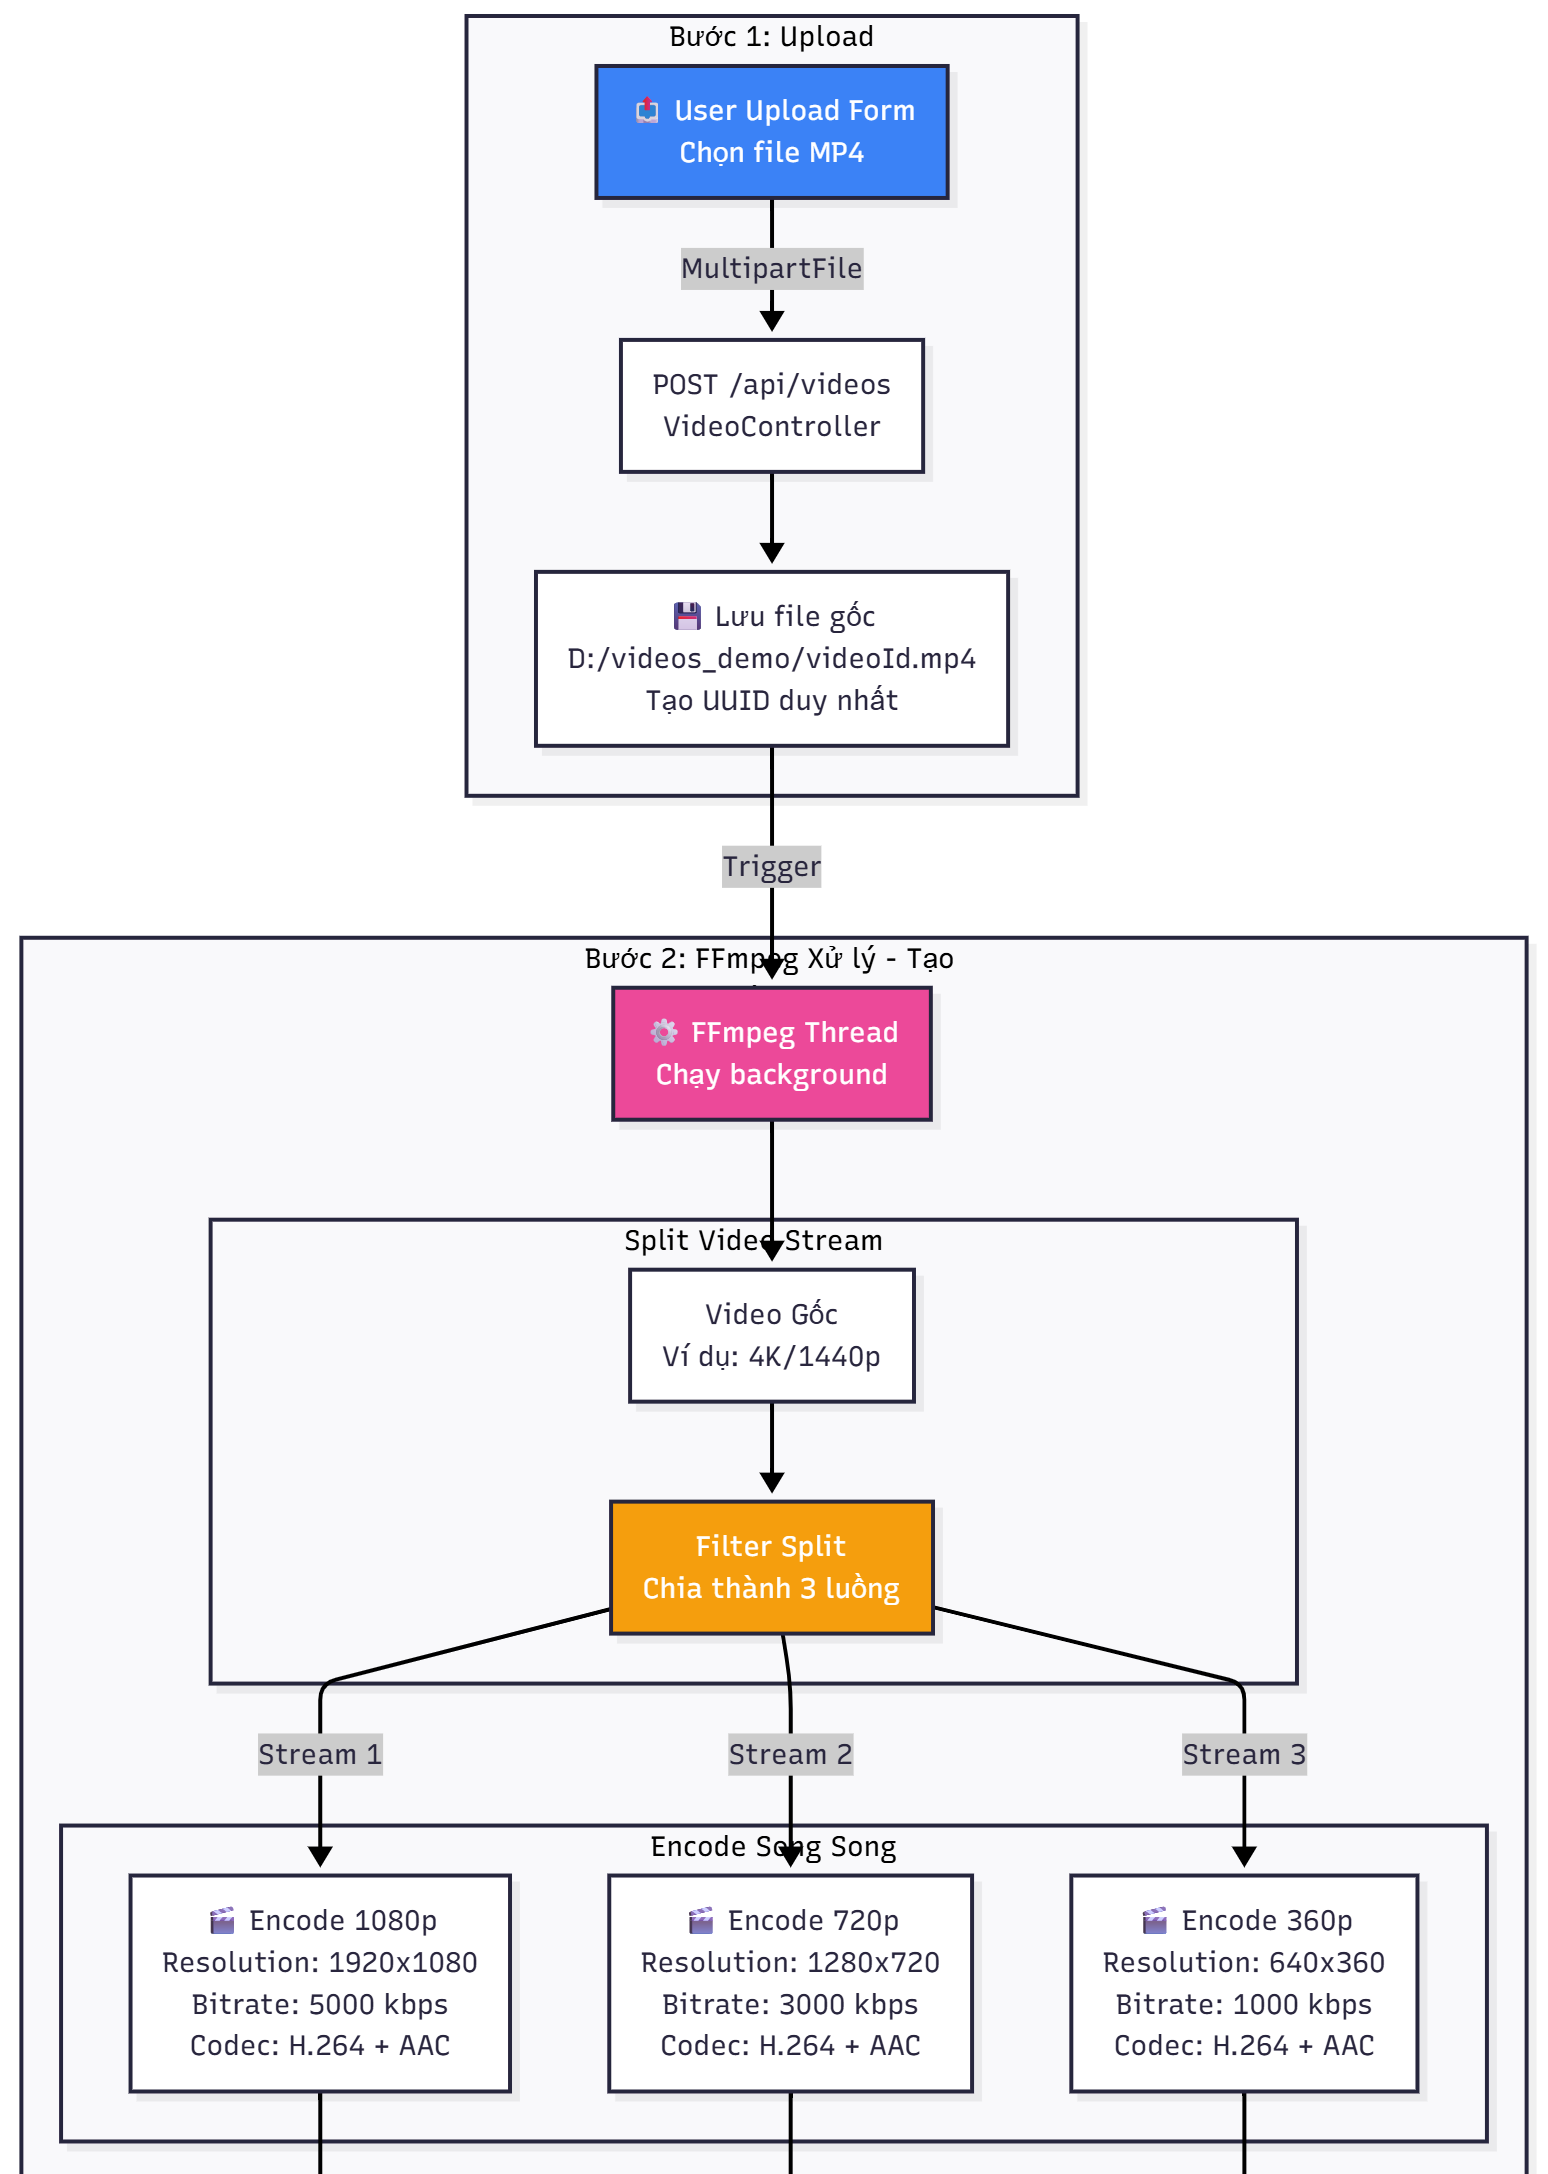
\includegraphics[width=1\textwidth]{image/mermaid/luongxulyvideo.png}
	\caption{Luồng xử lý video trong hệ thống NicePhim}
	\label{fig:luongxulyvideo}
\end{figure}

\begin{figure}[H]
	\centering
	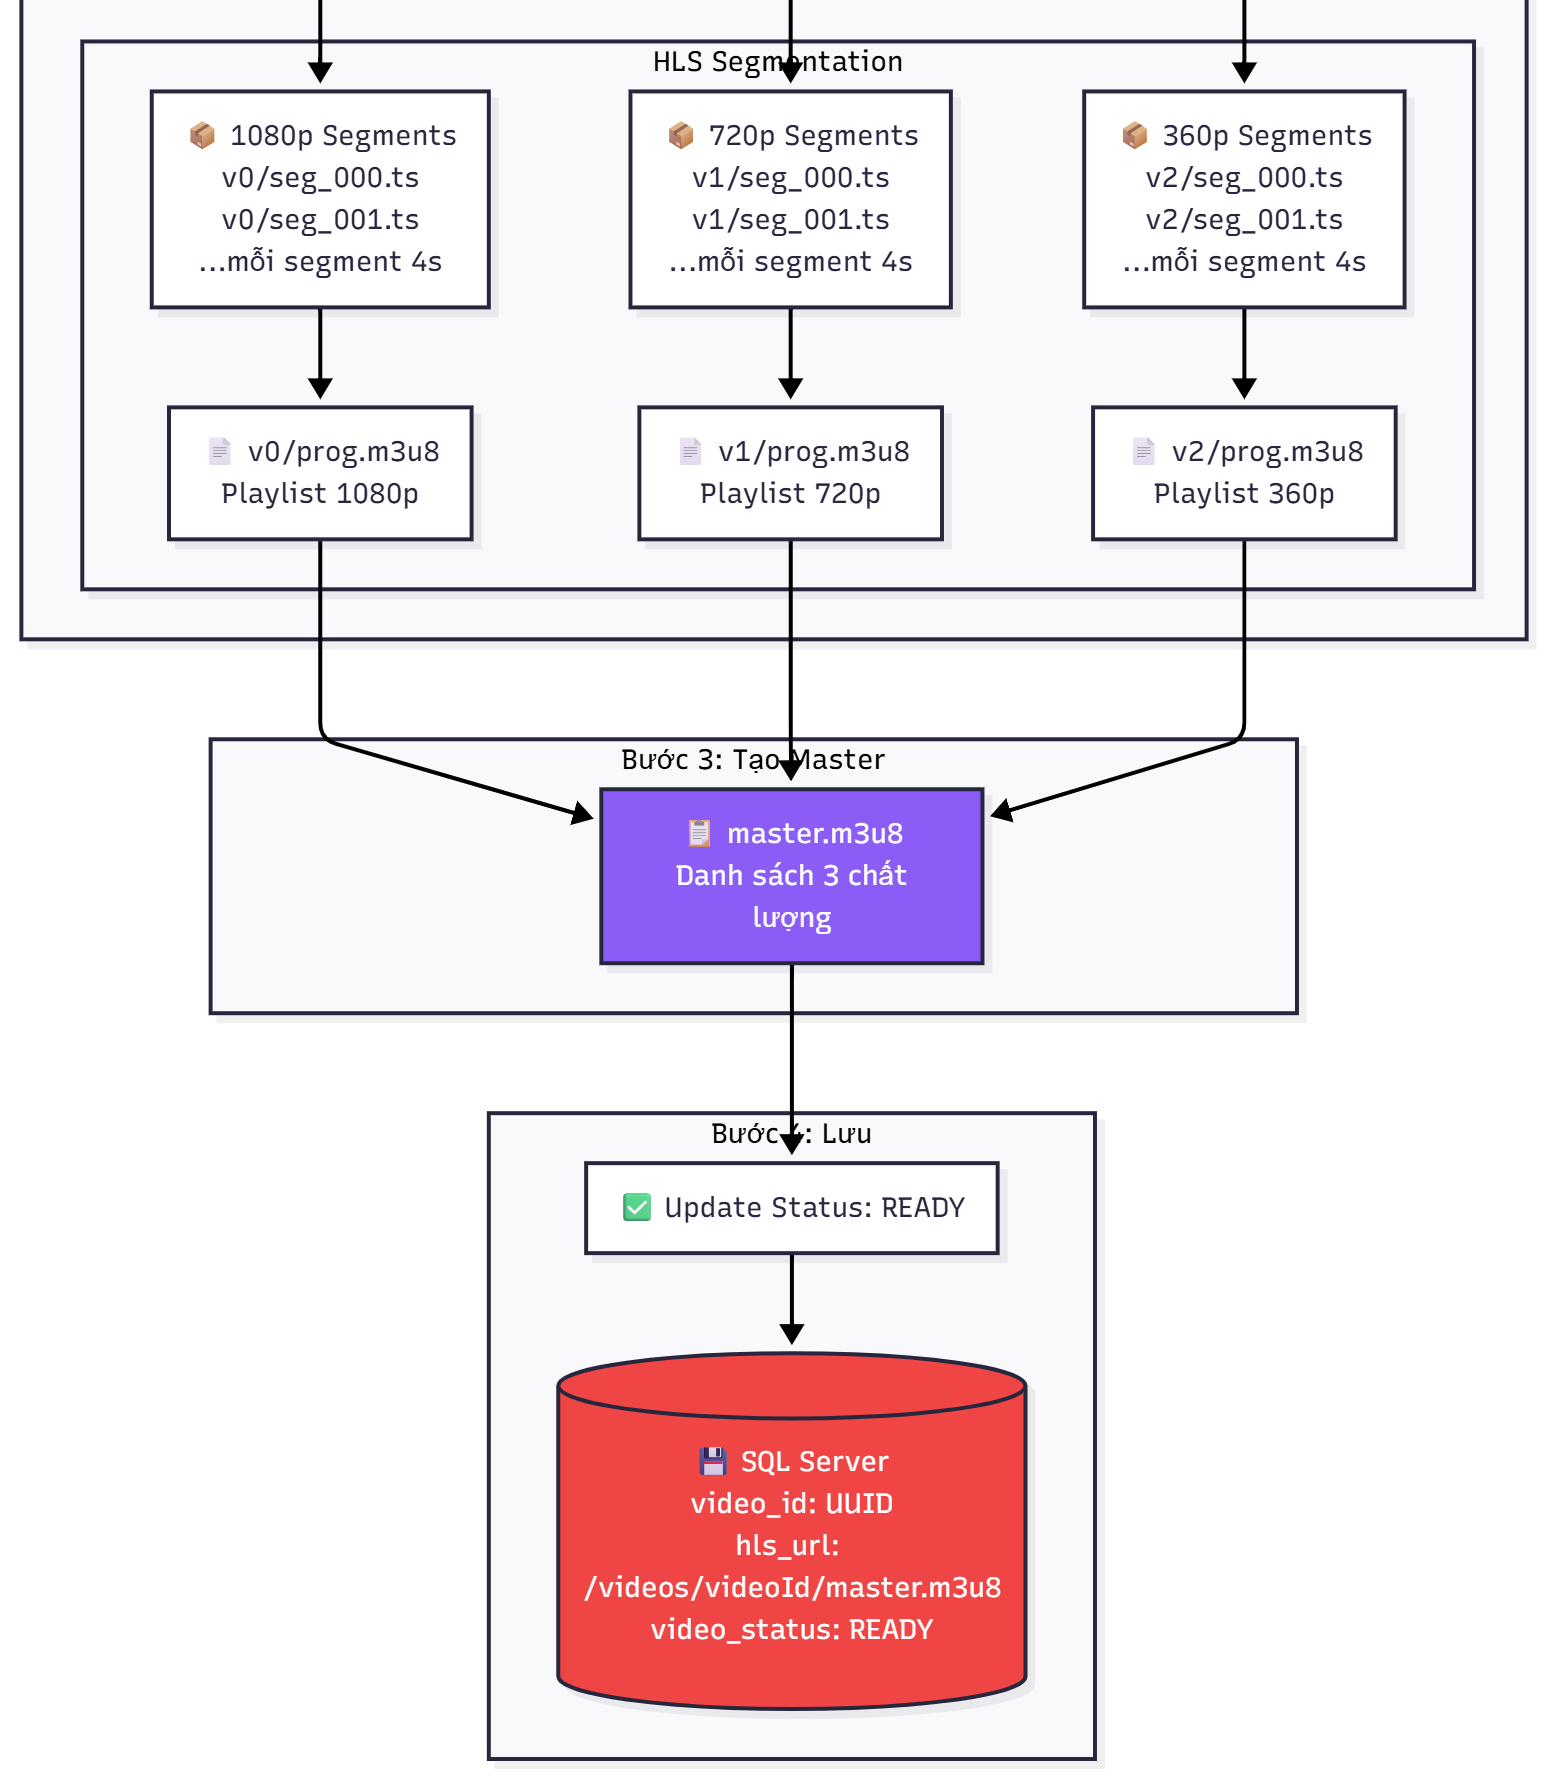
\includegraphics[width=1\textwidth]{image/mermaid/luongxulyvideo2.png}
	\caption{Luồng xử lý video trong hệ thống NicePhim}
	\label{fig:luongxulyvideo2}
\end{figure}

\subsection{Luồng phát video HLS}

\begin{figure}[H]
	\centering
	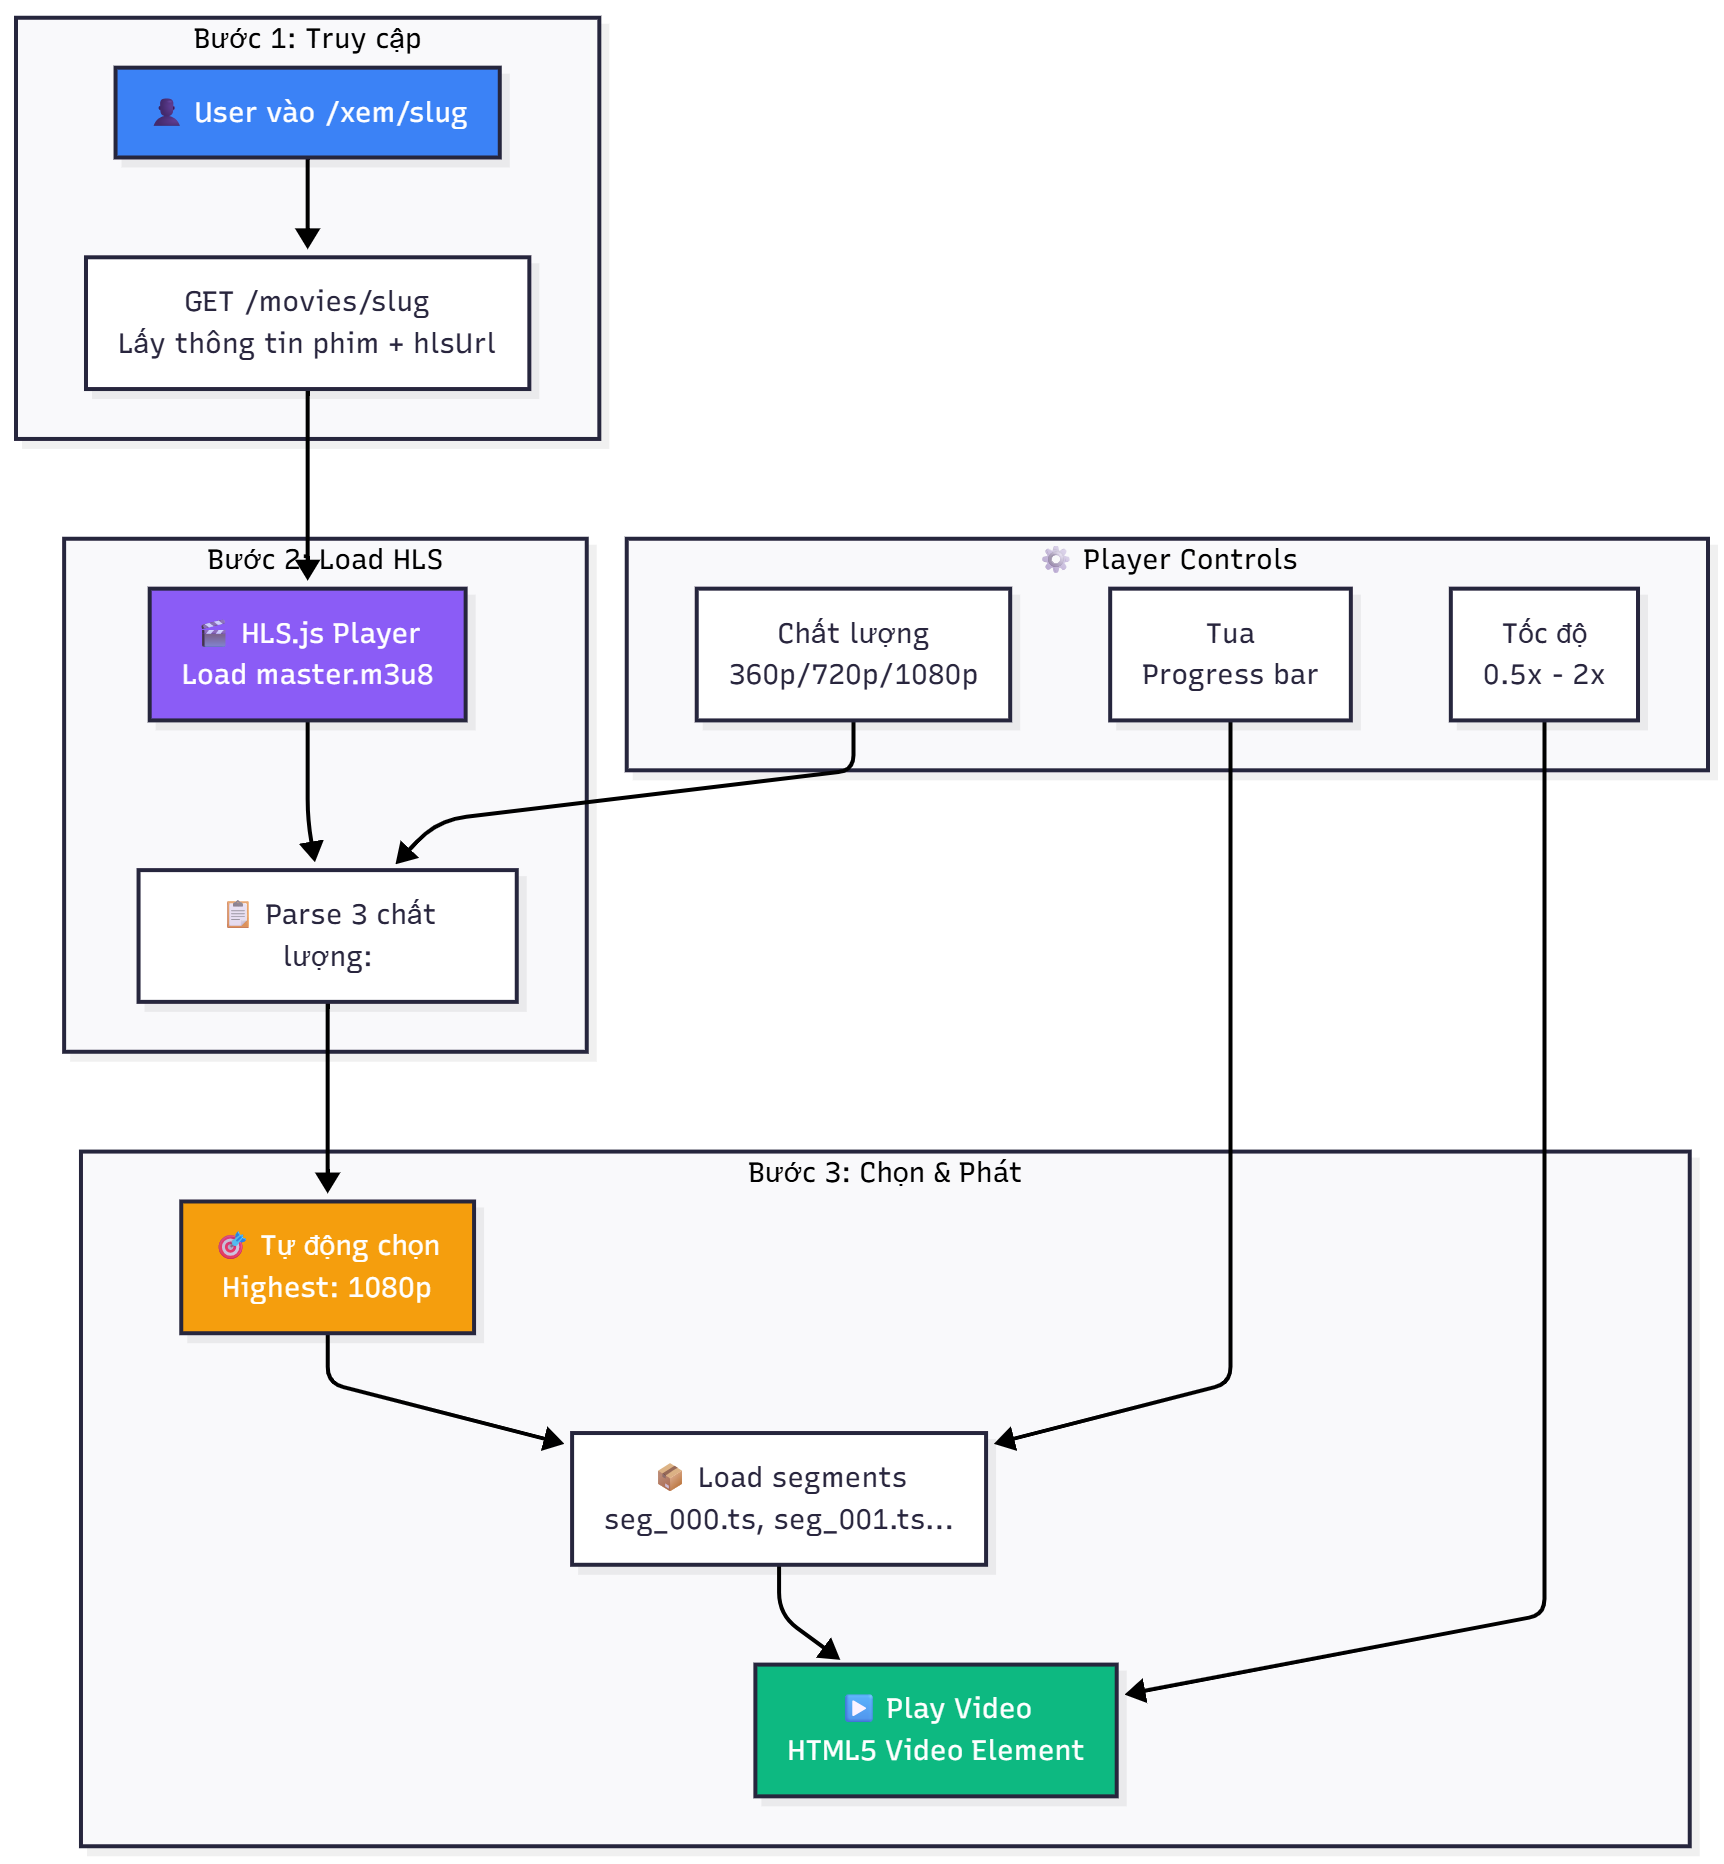
\includegraphics[width=1\textwidth]{image/mermaid/luongphatvideoHLS.png}
	\caption{Luồng phát video HLS trong hệ thống NicePhim}
	\label{fig:luongphatvideoHLS}
\end{figure}

\subsection{Luồng xem phim chung}

\begin{figure}[H]
	\centering
	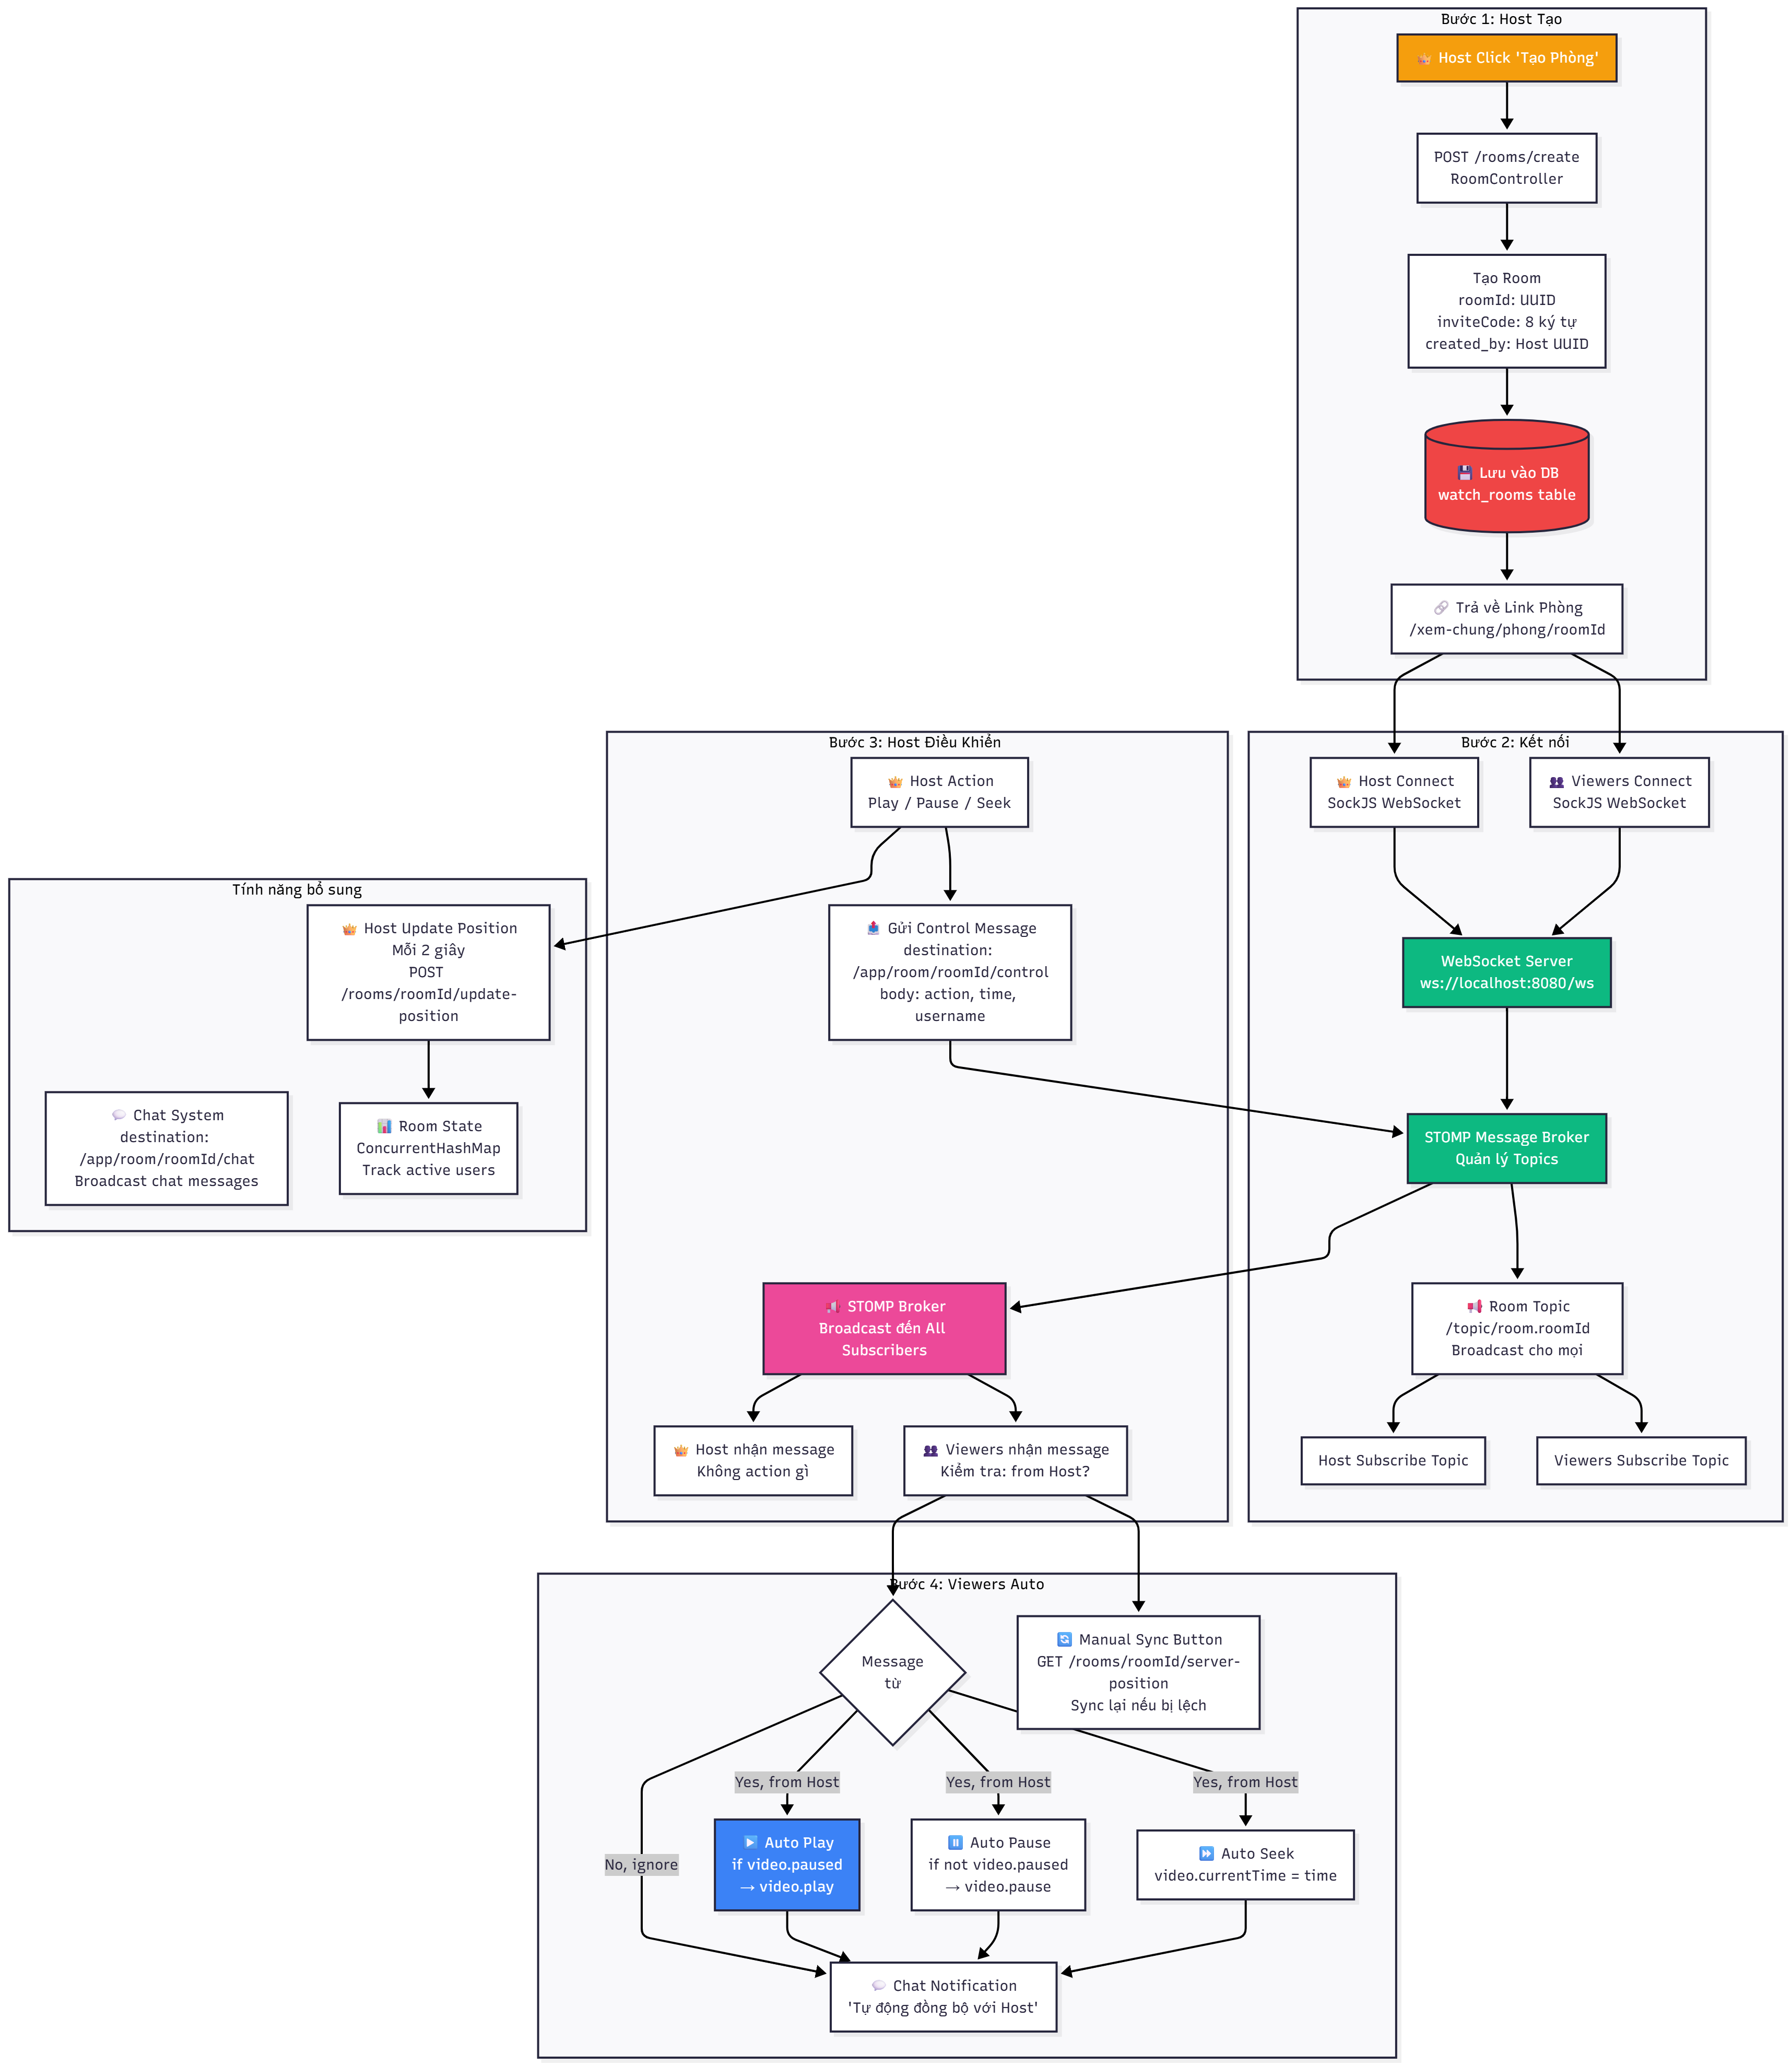
\includegraphics[width=1\textwidth]{image/mermaid/luongwatchtogether.png}
	\caption{Luồng xem phim chung trong hệ thống NicePhim}
	\label{fig:luongwatchtogether}
\end{figure}

\subsection{Luồng chat}

\begin{figure}[H]
	\centering
	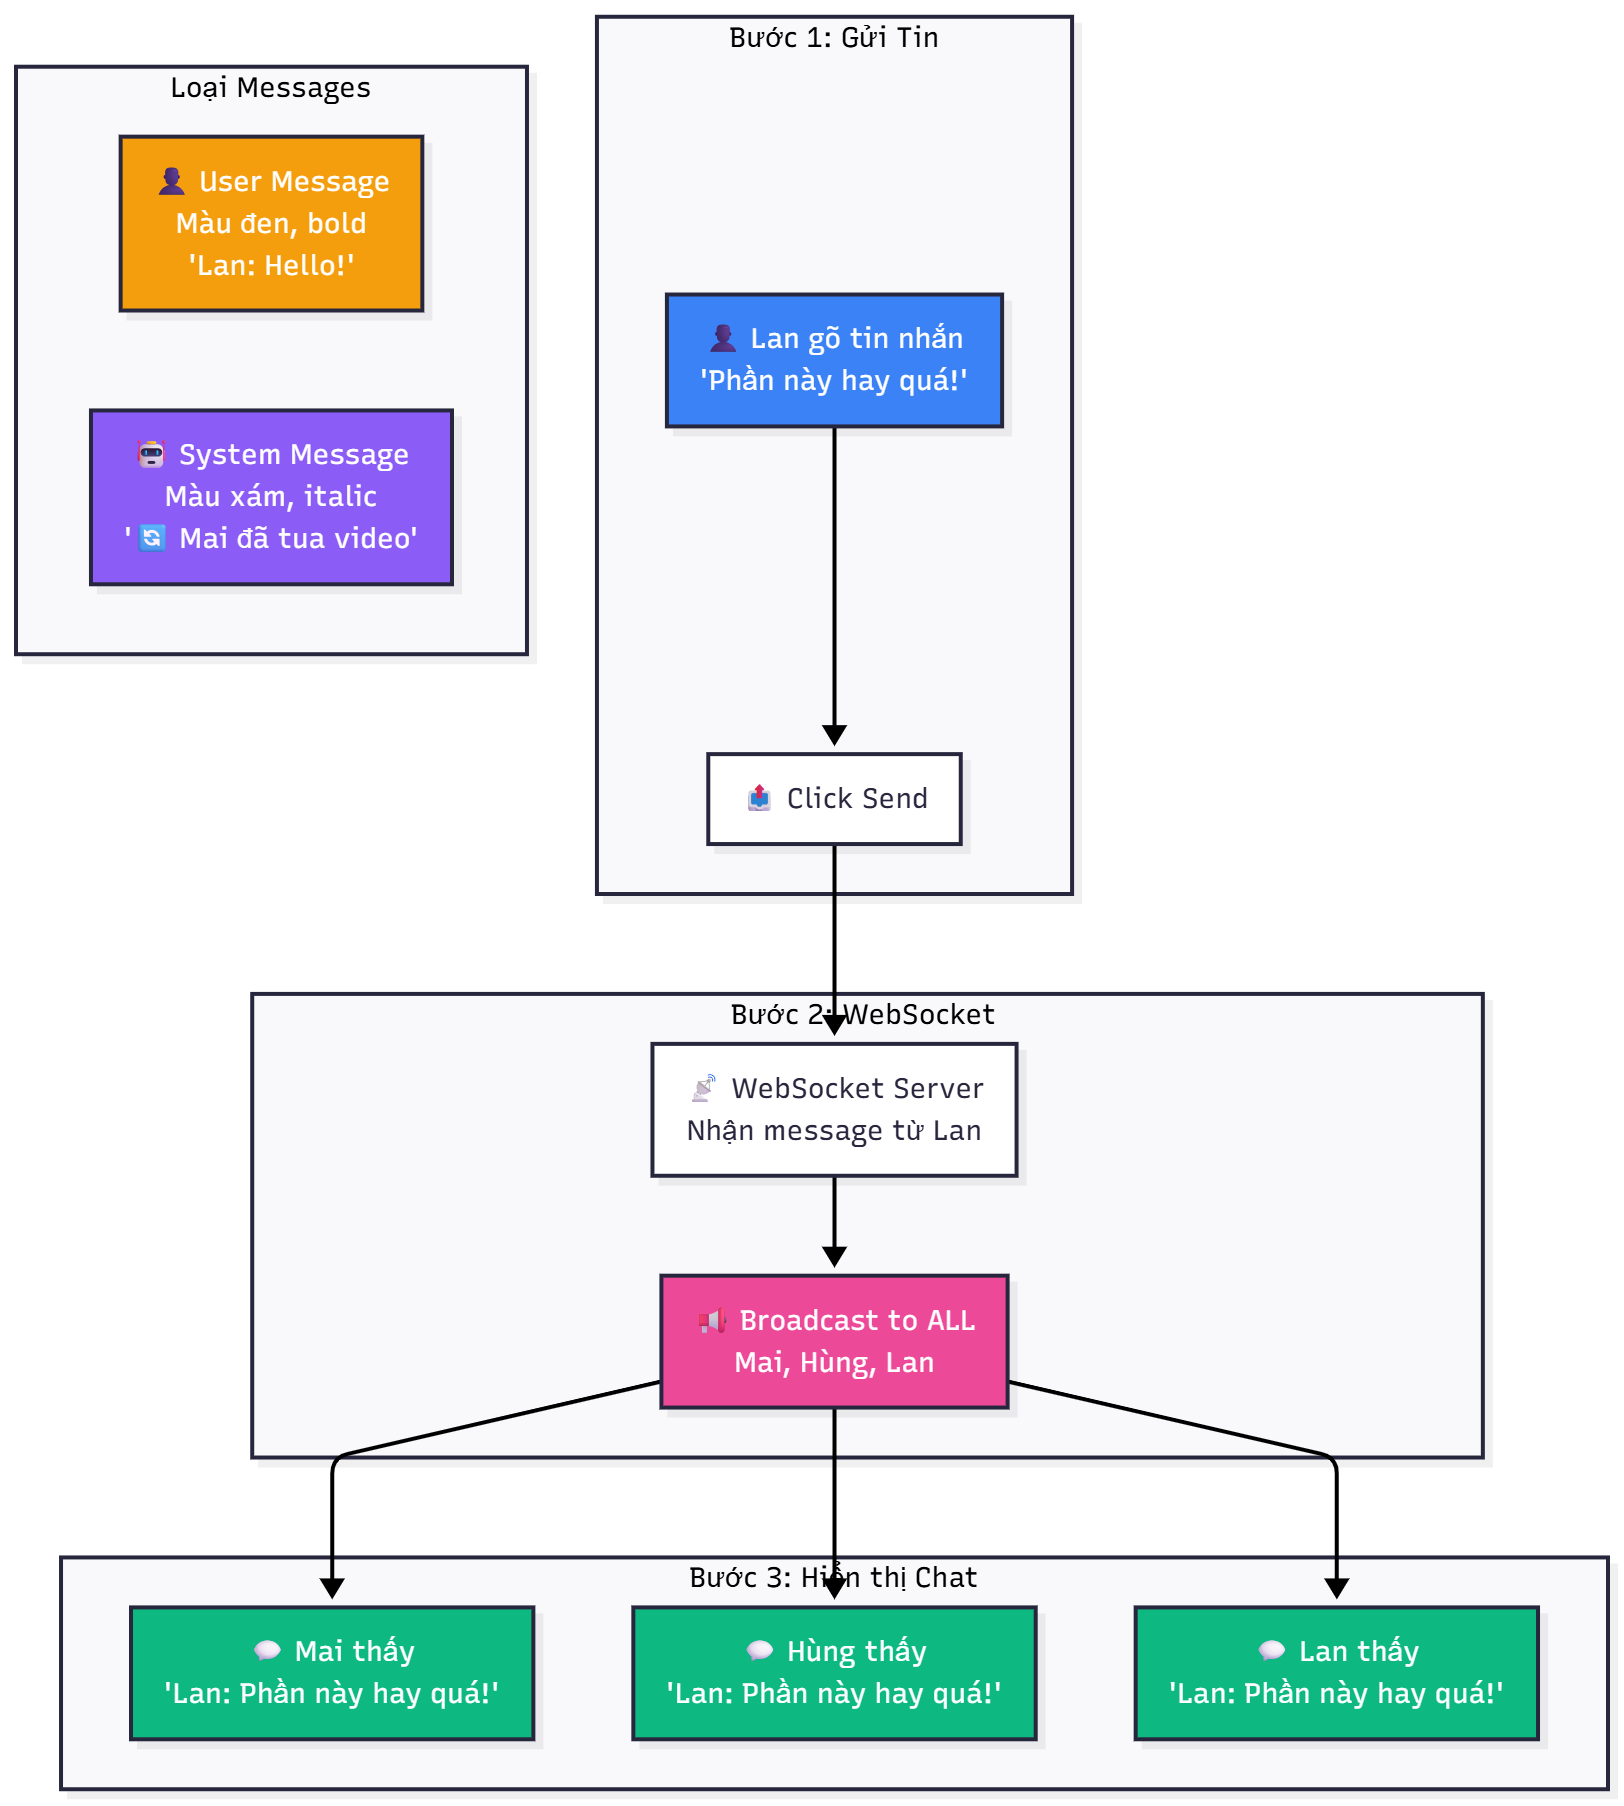
\includegraphics[width=1\textwidth]{image/mermaid/chat.png}
	\caption{Luồng chat trong hệ thống NicePhim}
	\label{fig:chat}
\end{figure}

\subsection{Cơ sở dữ liệu}

NicePhim sử dụng Microsoft SQL Server làm hệ quản trị cơ sở dữ liệu quan hệ. Database được thiết kế với 5 bảng chính để lưu trữ và quản lý dữ liệu của hệ thống. Các bảng được liên kết với nhau thông qua khóa ngoại (Foreign Key), đảm bảo tính toàn vẹn dữ liệu và hỗ trợ các truy vấn phức tạp. Tất cả các bảng sử dụng \texttt{uniqueidentifier} (UUID) làm khóa chính để đảm bảo tính duy nhất toàn cục và khả năng mở rộng.

Mối quan hệ giữa các bảng:
\begin{itemize}
	\item \textbf{users} tạo nhiều \textbf{movies} (1-nhiều)
	\item \textbf{users} tạo nhiều \textbf{watch\_rooms} (1-nhiều)
	\item \textbf{movies} thuộc nhiều \textbf{genres} thông qua bảng trung gian \textbf{movie\_genres} (nhiều-nhiều)
	\item \textbf{movies} được xem trong nhiều \textbf{watch\_rooms} (1-nhiều)
\end{itemize}

\subsubsection{Bảng users}

Bảng \texttt{users} lưu trữ thông tin người dùng của hệ thống, bao gồm thông tin xác thực và profile.

\begin{center}
	\small
	\begin{longtable}{|c|p{3.5cm}|p{2.5cm}|p{3cm}|p{3.5cm}|}
		\caption{Cấu trúc bảng users} \label{tab:users}                                                                     \\
		\hline
		\textbf{STT} & \textbf{Tên trường} & \textbf{Kiểu dữ liệu} & \textbf{Ràng buộc}       & \textbf{Mô tả}              \\
		\hline
		\endfirsthead

		\multicolumn{5}{c}%
		{{\tablename\ \thetable{} -- tiếp theo trang trước}}                                                                \\
		\hline
		\textbf{STT} & \textbf{Tên trường} & \textbf{Kiểu dữ liệu} & \textbf{Ràng buộc}       & \textbf{Mô tả}              \\
		\hline
		\endhead

		\hline \multicolumn{5}{r}{{Tiếp trang sau}}                                                                         \\
		\endfoot

		\hline
		\endlastfoot

		1            & user\_id            & uniqueidentifier      & PK                       & Mã định danh người dùng     \\
		\hline
		2            & username            & nvarchar(255)         & UK, NOT NULL             & Tên đăng nhập duy nhất      \\
		\hline
		3            & email               & nvarchar(255)         & UK, NOT NULL             & Địa chỉ email duy nhất      \\
		\hline
		4            & password\_hash      & varbinary(MAX)        & NOT NULL                 & Mật khẩu đã mã hóa BCrypt   \\
		\hline
		5            & display\_name       & nvarchar(255)         &                          & Tên hiển thị của người dùng \\
		\hline
		6            & avatar\_url         & nvarchar(500)         &                          & URL ảnh đại diện            \\
		\hline
		7            & is\_admin           & bit                   & DEFAULT 0                & Quyền quản trị viên         \\
		\hline
		8            & created\_at         & datetime2             & DEFAULT SYSUTCDATETIME() & Thời gian tạo tài khoản     \\
		\hline
		9            & updated\_at         & datetime2             &                          & Thời gian cập nhật cuối     \\
		\hline
	\end{longtable}
\end{center}

\subsubsection{Bảng movies}

Bảng \texttt{movies} lưu trữ thông tin chi tiết về các bộ phim trong hệ thống, bao gồm metadata và đường dẫn video.

\begin{center}
	\small
	\begin{longtable}{|c|p{3cm}|p{2.5cm}|p{3cm}|p{4cm}|}
		\caption{Cấu trúc bảng movies} \label{tab:movies}                                                                      \\
		\hline
		\textbf{STT} & \textbf{Tên trường} & \textbf{Kiểu dữ liệu} & \textbf{Ràng buộc}       & \textbf{Mô tả}                 \\
		\hline
		\endfirsthead

		\multicolumn{5}{c}%
		{{\tablename\ \thetable{} -- tiếp theo trang trước}}                                                                   \\
		\hline
		\textbf{STT} & \textbf{Tên trường} & \textbf{Kiểu dữ liệu} & \textbf{Ràng buộc}       & \textbf{Mô tả}                 \\
		\hline
		\endhead

		\hline \multicolumn{5}{r}{{Tiếp trang sau}}                                                                            \\
		\endfoot

		\hline
		\endlastfoot

		1            & movie\_id           & uniqueidentifier      & PK                       & Mã định danh phim              \\
		\hline
		2            & title               & nvarchar(255)         & NOT NULL                 & Tiêu đề phim                   \\
		\hline
		3            & alias\_title        & nvarchar(255)         &                          & Tiêu đề phụ hoặc tên gốc       \\
		\hline
		4            & description         & nvarchar(MAX)         &                          & Mô tả nội dung phim            \\
		\hline
		5            & release\_year       & smallint              &                          & Năm phát hành                  \\
		\hline
		6            & age\_rating         & nvarchar(10)          &                          & Giới hạn độ tuổi (PG, R, etc.) \\
		\hline
		7            & imdb\_rating        & decimal(3,1)          &                          & Điểm đánh giá IMDB             \\
		\hline
		8            & is\_series          & bit                   & DEFAULT 0                & Phân biệt phim lẻ/phim bộ      \\
		\hline
		9            & poster\_url         & nvarchar(500)         &                          & URL hình poster                \\
		\hline
		10           & banner\_url         & nvarchar(500)         &                          & URL hình banner                \\
		\hline
		11           & created\_by         & uniqueidentifier      & FK (users), NOT NULL     & Người tạo phim                 \\
		\hline
		12           & video\_id           & nvarchar(100)         &                          & ID video trong storage         \\
		\hline
		13           & hls\_url            & nvarchar(500)         &                          & URL manifest HLS (.m3u8)       \\
		\hline
		14           & video\_status       & nvarchar(20)          &                          & Trạng thái xử lý video         \\
		\hline
		15           & created\_at         & datetime2             & DEFAULT SYSUTCDATETIME() & Thời gian tạo                  \\
		\hline
		16           & updated\_at         & datetime2             &                          & Thời gian cập nhật cuối        \\
		\hline
	\end{longtable}
\end{center}

\subsubsection{Bảng genres}

Bảng \texttt{genres} lưu trữ danh sách các thể loại phim có trong hệ thống.

\begin{center}
	\small
	\begin{longtable}{|c|p{4cm}|p{3cm}|p{3cm}|p{4cm}|}
		\caption{Cấu trúc bảng genres} \label{tab:genres}                                                                    \\
		\hline
		\textbf{STT} & \textbf{Tên trường} & \textbf{Kiểu dữ liệu} & \textbf{Ràng buộc} & \textbf{Mô tả}                     \\
		\hline
		\endfirsthead

		\multicolumn{5}{c}%
		{{\tablename\ \thetable{} -- tiếp theo trang trước}}                                                                 \\
		\hline
		\textbf{STT} & \textbf{Tên trường} & \textbf{Kiểu dữ liệu} & \textbf{Ràng buộc} & \textbf{Mô tả}                     \\
		\hline
		\endhead

		\hline \multicolumn{5}{r}{{Tiếp trang sau}}                                                                          \\
		\endfoot

		\hline
		\endlastfoot

		1            & genre\_id           & uniqueidentifier      & PK                 & Mã định danh thể loại              \\
		\hline
		2            & name                & nvarchar(100)         & UK, NOT NULL       & Tên thể loại (Action, Drama, etc.) \\
		\hline
	\end{longtable}
\end{center}

\subsubsection{Bảng movie\_genres}

Bảng \texttt{movie\_genres} là bảng trung gian (junction table) thiết lập mối quan hệ nhiều-nhiều giữa \texttt{movies} và \texttt{genres}, cho phép một phim thuộc nhiều thể loại và một thể loại chứa nhiều phim.

\begin{center}
	\small
	\begin{longtable}{|c|p{4cm}|p{3cm}|p{3cm}|p{4cm}|}
		\caption{Cấu trúc bảng movie\_genres} \label{tab:movie_genres}                                          \\
		\hline
		\textbf{STT} & \textbf{Tên trường} & \textbf{Kiểu dữ liệu} & \textbf{Ràng buộc} & \textbf{Mô tả}        \\
		\hline
		\endfirsthead

		\multicolumn{5}{c}%
		{{\tablename\ \thetable{} -- tiếp theo trang trước}}                                                    \\
		\hline
		\textbf{STT} & \textbf{Tên trường} & \textbf{Kiểu dữ liệu} & \textbf{Ràng buộc} & \textbf{Mô tả}        \\
		\hline
		\endhead

		\hline \multicolumn{5}{r}{{Tiếp trang sau}}                                                             \\
		\endfoot

		\hline
		\endlastfoot

		1            & movie\_id           & uniqueidentifier      & PK, FK (movies)    & Mã định danh phim     \\
		\hline
		2            & genre\_id           & uniqueidentifier      & PK, FK (genres)    & Mã định danh thể loại \\
		\hline
	\end{longtable}
\end{center}

\textit{Lưu ý: Bảng này sử dụng composite primary key gồm cả movie\_id và genre\_id.}

\subsubsection{Bảng watch\_rooms}

Bảng \texttt{watch\_rooms} lưu trữ thông tin về các phòng xem chung, bao gồm trạng thái phát video được đồng bộ giữa các thành viên.

\begin{center}
	\small
	\begin{longtable}{|c|p{3cm}|p{2.5cm}|p{3.5cm}|p{4cm}|}
		\caption{Cấu trúc bảng watch\_rooms} \label{tab:watch_rooms}                                                                 \\
		\hline
		\textbf{STT} & \textbf{Tên trường} & \textbf{Kiểu dữ liệu} & \textbf{Ràng buộc}       & \textbf{Mô tả}                       \\
		\hline
		\endfirsthead

		\multicolumn{5}{c}%
		{{\tablename\ \thetable{} -- tiếp theo trang trước}}                                                                         \\
		\hline
		\textbf{STT} & \textbf{Tên trường} & \textbf{Kiểu dữ liệu} & \textbf{Ràng buộc}       & \textbf{Mô tả}                       \\
		\hline
		\endhead

		\hline \multicolumn{5}{r}{{Tiếp trang sau}}                                                                                  \\
		\endfoot

		\hline
		\endlastfoot

		1            & room\_id            & uniqueidentifier      & PK                       & Mã định danh phòng                   \\
		\hline
		2            & name                & nvarchar(255)         & NOT NULL                 & Tên phòng xem chung                  \\
		\hline
		3            & created\_by         & uniqueidentifier      & FK (users), NOT NULL     & Người tạo phòng                      \\
		\hline
		4            & movie\_id           & uniqueidentifier      & FK (movies)              & Phim đang xem trong phòng            \\
		\hline
		5            & current\_time\_ms   & bigint                & DEFAULT 0                & Vị trí video hiện tại (milliseconds) \\
		\hline
		6            & playback\_state     & tinyint               & DEFAULT 0                & Trạng thái phát (0: pause, 1: play)  \\
		\hline
		7            & playback\_rate      & decimal(3,2)          & DEFAULT 1.0              & Tốc độ phát (0.5x, 1x, 2x, etc.)     \\
		\hline
		8            & created\_at         & datetime2             & DEFAULT SYSUTCDATETIME() & Thời gian tạo phòng                  \\
		\hline
		9            & updated\_at         & datetime2             &                          & Thời gian cập nhật cuối              \\
		\hline
		10           & row\_version        & timestamp             &                          & Optimistic concurrency control       \\
		\hline
	\end{longtable}
\end{center}


\newpage
% CHƯƠNG 5: KẾT QUẢ THỰC NGHIỆM

\section{\textbf{CHƯƠNG 5: KẾT QUẢ THỰC NGHIỆM}}

\subsection{Giới thiệu}
Chương này trình bày các kết quả thực nghiệm thực tế trong quá trình phát triển và triển khai hệ thống NicePhim. Các thử nghiệm tập trung vào hiệu năng streaming, khả năng upload video lớn, tính năng xem phim cá nhân và xem chung (Watch Together), cũng như trải nghiệm giao diện người dùng.

\subsection{1. Thực nghiệm streaming đa chất lượng và upload video lớn}
\begin{itemize}
	\item \textbf{Streaming đa chất lượng:} Hệ thống sử dụng FFmpeg để chuyển đổi video sang HLS với nhiều mức chất lượng (360p, 720p, 1080p). Thực nghiệm cho thấy người dùng có thể chuyển đổi chất lượng mượt mà, không gián đoạn.
	\item \textbf{Upload video lớn:} Đã kiểm thử upload thành công các file video lên tới 500MB, hệ thống backend xử lý và chuyển đổi ổn định, không phát sinh lỗi.
	\item \textbf{Tối ưu trình phát:} Trình phát SimpleHLSPlayer hỗ trợ chọn chất lượng, tua nhanh/chậm, toàn màn hình, ghi nhớ tiến trình xem.
\end{itemize}

\subsection{2. Thực nghiệm tính năng xem chung (Watch Together)}
\begin{itemize}
	\item \textbf{Đồng bộ thời gian thực:} Tính năng xem chung hoạt động ổn định, đồng bộ phát video giữa các thành viên qua WebSocket (STOMP), kể cả khi có thành viên mới tham gia giữa chừng.
	\item \textbf{Chat realtime:} Tích hợp chat trực tiếp trong phòng xem chung, kiểm thử với nhiều user cho kết quả phản hồi tức thì.
	\item \textbf{Quản lý phòng:} Tạo/join phòng, quản lý thành viên, phân quyền quản trị phòng hoạt động đúng như thiết kế.
\end{itemize}

\subsection{3. Thực nghiệm giao diện và trải nghiệm người dùng}
\begin{itemize}
	\item \textbf{Giao diện responsive:} Giao diện NicePhim hiển thị tốt trên cả máy tính và thiết bị di động, tối ưu thao tác người dùng.
	\item \textbf{Đăng ký/Đăng nhập:} Quy trình đăng ký, đăng nhập, xác thực hoạt động ổn định, thông báo lỗi rõ ràng.
	\item \textbf{Quản lý phim/thể loại:} Chức năng thêm, sửa, xoá phim và thể loại qua giao diện admin hoạt động đúng yêu cầu (nếu có).
\end{itemize}

\subsection{Tổng kết chương}
Các kết quả thực nghiệm đã chứng minh hệ thống NicePhim đáp ứng tốt các yêu cầu về hiệu năng streaming, đồng bộ xem chung, upload video lớn và trải nghiệm người dùng. Việc kiểm thử thực tế với các tình huống đa dạng giúp hoàn thiện sản phẩm, sẵn sàng triển khai và phục vụ người dùng cuối.


\newpage
\section{\textbf{CHƯƠNG 6: KẾT LUẬN VÀ KIẾN NGHỊ}}


\subsection{Kết Luận}

\subsubsection{Tổng kết quá trình thực hiện đồ án}
Đồ án đã thực hiện xây dựng thành công mạng xã hội Honey Social với kiến trúc hiện đại, tách biệt Frontend và Backend rõ ràng. Quá trình phát triển tuân theo phương pháp Agile, cho phép linh hoạt điều chỉnh khi gặp thách thức. Việc áp dụng các mô hình thiết kế như MVC, đã giúp mã nguồn có cấu trúc tốt, dễ bảo trì và mở rộng.

\subsubsection{Kết quả đạt được}
\begin{enumerate}
    \item \textbf{Hệ thống đa chức năng} - Mạng xã hội hoàn chỉnh với các tính năng chính:
    \begin{itemize}
        \item Đăng bài viết với hình ảnh và văn bản
        \item Hệ thống chat realtime giữa người dùng
        \item Trợ lý AI thông minh tích hợp
        \item Hệ thống gợi ý nội dung dựa trên vector search
        \item Hệ thống thông báo realtime
        \item Tìm kiếm nâng cao với Elasticsearch
    \end{itemize}
    
    \item \textbf{Kiến trúc kỹ thuật hiện đại}:
    \begin{itemize}
        \item Frontend: React.js với state management thông qua Redux
        \item Backend: Node.js, Express.js với TypeScript
        \item Cơ sở dữ liệu: MongoDB kết hợp với Redis cache
        \item WebSocket cho giao tiếp realtime
        \item RabbitMQ cho hàng đợi xử lý bất đồng bộ
        \item Docker cho việc phát triển và triển khai
    \end{itemize}
    
    \item \textbf{Hiệu năng cao}:
    \begin{itemize}
        \item Hệ thống cache đa tầng giúp giảm tải database
        \item Xử lý bất đồng bộ các tác vụ nặng như phân tích nội dung, moderation
        \item Vector search cho khả năng tìm kiếm và gợi ý thông minh
    \end{itemize}
\end{enumerate}

\subsubsection{Hạn chế và thách thức}
\begin{enumerate}
    \item \textbf{Độ phức tạp của hệ thống}:
    \begin{itemize}
        \item Cache invalidation khó xử lý đúng trong mọi tình huống
        \item Phân tán microservice làm tăng độ phức tạp vận hành
    \end{itemize}
    
    \item \textbf{Hiệu năng của AI}:
    \begin{itemize}
        \item Thời gian phản hồi của ChatAI đôi khi còn chậm
        \item Vector embedding tốn kém tài nguyên khi hệ thống lớn
    \end{itemize}
    
    \item \textbf{Giới hạn tích hợp}:
    \begin{itemize}
        \item Chưa có ứng dụng di động native
        \item Hệ thống gợi ý cần thêm dữ liệu để tăng độ chính xác
    \end{itemize}
\end{enumerate}

\subsection{Kiến nghị và hướng phát triển}

\subsubsection{Phát triển ứng dụng di động}
Xây dựng ứng dụng di động native cho iOS và Android sử dụng React Native hoặc Flutter để tận dụng codebase hiện có, đồng thời cải thiện trải nghiệm người dùng trên thiết bị di động với các tính năng như thông báo đẩy, camera tích hợp và trải nghiệm offline.

\subsubsection{Nâng cấp hệ thống gợi ý nội dung}
Cải tiến hệ thống gợi ý bằng cách kết hợp các yếu tố hành vi người dùng (thời gian xem, tương tác), ngữ cảnh (thời gian, vị trí) và mạng xã hội (kết nối giữa người dùng) để tạo ra gợi ý cá nhân hóa chính xác hơn.

\subsubsection{Triển khai AI Chatbot học tự động}
Phát triển khả năng học tự động cho ChatAI để liên tục cải thiện chất lượng phản hồi dựa trên tương tác của người dùng. Triển khai fine-tuning mô hình để chatbot hiểu tốt hơn ngữ cảnh và văn hóa cụ thể của cộng đồng Honey Social.

\subsubsection{Tối ưu cơ chế làm mới Redis Cache}
Cải tiến cơ chế cache với chiến lược write-through và read-through thông minh hơn, đồng thời sử dụng Redis Streams để quản lý việc làm mới cache phân tán, giảm thiểu lỗi cache inconsistency trong hệ thống nhiều node.

\subsubsection{Cải tiến hệ thống Post Recommendation}
Nâng cấp hệ thống gợi ý bài đăng bằng cách sử dụng kỹ thuật collaborative filtering kết hợp với vector search, đồng thời tối ưu hóa thuật toán lọc bọt (filter bubble) để đảm bảo người dùng tiếp cận được nhiều nội dung đa dạng.

\subsubsection{Phát triển ChatboxAI nội bộ}
Xây dựng công cụ chatbot nội bộ được huấn luyện trên dữ liệu hệ thống để hỗ trợ người quản trị trong việc phân tích xu hướng, phát hiện nội dung vi phạm, và tổng hợp báo cáo hoạt động của cộng đồng.
\clearpage
\section{TÀI LIỆU THAM KHẢO}
\begin{thebibliography}{00}

\bibitem{aws-doc}
Amazon Web Services, "Deploy a React-based single-page application to Amazon S3 and CloudFront." [Online].\\
Available: \url{https://short.com.vn/P0gh}

\bibitem{openai-moderation}
OpenAI, "Moderation Guide." [Online].\\
Available: \url{https://platform.openai.com/docs/guides/moderation}

\bibitem{openai-assistants}
OpenAI, "Assistants API Overview." [Online].\\
Available: \url{https://platform.openai.com/docs/assistants/overview}

\bibitem{openai-embeddings}
OpenAI, "Embeddings Guide." [Online].\\
Available: \url{https://platform.openai.com/docs/guides/embeddings}

\bibitem{cache-aside}
GeeksforGeeks, "Cache-Aside Pattern." [Online].\\
Available: \url{https://www.geeksforgeeks.org/cache-aside-pattern/}

\bibitem{elasticsearch-knowi}
Knowi, "What is Elasticsearch?" [Online].\\
Available: \url{https://www.knowi.com/blog/what-is-elastic-search/}

\end{thebibliography}

\end{document}